\documentclass[a4paper,12pt]{report}
\usepackage{listings}
\usepackage[utf8]{inputenc}
\usepackage{textcomp}
\usepackage[english,russian]{babel}
\usepackage[T2A]{fontenc}
\usepackage{xcolor}
\usepackage{hyperref}
\usepackage{indentfirst}
\usepackage{amssymb}
\usepackage{amsmath}
\usepackage{courier}
\usepackage{graphicx}
\usepackage{wrapfig}


\lstset{literate=%
    {é}{{\'e}}1
    {Ô}{{\^O}}1
}
\newcommand\mytilde{\char`\~}
\lstset{extendedchars=\true}
\lstset{inputencoding=ansinew}

\setlength{\parindent}{1cm}

\definecolor{gray}{rgb}{0.8, 0.8, 0.8}
\definecolor{lgreen}{HTML}{EEFFCC}
\definecolor{lorange}{HTML}{FBF4E9}
\definecolor{lgray}{HTML}{EFF3F8}

\lstset{frame=single, language=Erlang, backgroundcolor=\color{gray}, basicstyle=\footnotesize\ttfamily, commentstyle=\color{green}}
\lstdefinestyle{repl}{
    frame=single, 
    language=erlang, 
    backgroundcolor=\color{lgray}, 
    basicstyle=\ttfamily, 
    columns=fixed, 
    commentstyle=\color{green}, 
    breaklines=true
}
\lstdefinestyle{erlang}{frame=single, language=Erlang, backgroundcolor=\color{lgray}, basicstyle=\footnotesize\ttfamily, commentstyle=\color{green}, breaklines=true, breakautoindent=true}

\graphicspath { {images/} }
\newcommand{\ops}{\colorbox{lgreen}}
\newcommand{\blankline}{\vspace{10pt}}


\begin{document}

\begin{titlepage}
    \begin{center}
        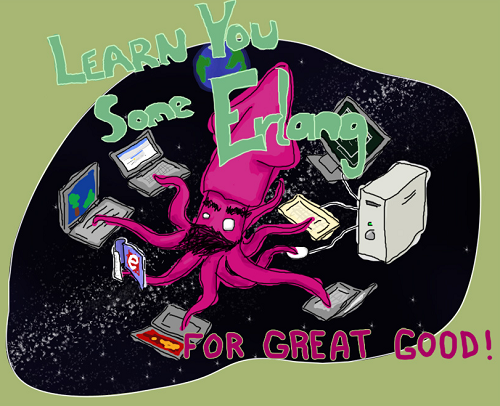
\includegraphics[width=1\textwidth]{title.png}
        \large Learn You Some Erlang for Great Good!\\
        Изучай Erlang во имя добра!
        \\[3cm]
        \begin{minipage}{1\textwidth}
                \large\emph{Автор:}
                 Frederic Trottier\--Hebert\\
        \end{minipage}
    \end{center}
    \vfill
    \begin{center}
        \emph{v. 0.14.1}
    \end{center}
\end{titlepage}

\chapter{Введение}\label{introduction}

\section{О книге}

Начни изучать Эрланг во имя добра!
Чтение этого руководства, скорее всего, будет одним из твоих первых шагов в изучении Erlang, поэтому скажу о нём пару слов.

\begin{wrapfigure}{l}{0.3\linewidth}
    
\includegraphics[width=1\linewidth]{erlang.png}
\end{wrapfigure}

Во\--первых, идея написать это обучающее руководство появилась у меня после того, как я прочитал \href{http://learnyouahaskell.com}{Изучай Haskell во имя добра!} Miran Lipova\v{c}a.
Мне показалось, что ему удалось представить язык в привлекательном свете, и сделать процесс обучения приятным.
Я уже был знаком с Мираном, поэтому поинтересовался, как он относится к тому, что я напишу версию его книги, посвящённую Erlang.
Идея пришлась ему по душе, так как он и сам интересовался Erlang.

Всё это привело к тому, что я теперь печатаю эти слова.
Конечно, были и другие источники мотивации: я считаю что <<порог вхождения>> в язык довольно высок (в web маловато документации и, скорее всего, придётся покупать книги).
Поэтому я подумал, что сообществу пригодится руководство похожее на LYAH.
Ещё я заметил, что люди приписывали Erlang слишком много или слишком мало достоинств, основываясь при этом на поверхностных суждениях.
Есть люди, которые абсолютно уверены, что Erlang это просто разрекламированная пустышка.
Даже если бы я хотел их убедить в обратном, знаю, что они вряд ли прочитают эти строки.

Эта книга даёт возможность изучить Erlang тем, кто имеет базовые знания о программировании на императивных языках (таких как C/C++, Java, Python, Ruby и т.д.) и имеет или не имеет представление о функциональном программировании (Haskell, Scala, Erlang, Clojure, OCaml\ldots)
Также я хочу, чтобы эта книга честно рассказывала об Erlang, правдиво освещая слабые и сильные стороны языка.

\section{Так что же такое Erlang?}
Во\--первых, Erlang это функциональный язык программирования.
Если вам приходилось когда\--либо работать с императивными языками, то вы нормально относитесь к выражениям вроде \ops{i++;} в функциональном программировании такие выражения не разрешаются.
Более того, изменять значение любой переменной строго запрещено!
Сначала это может прозвучать странно, но если вы припомните уроки математики, то на них всё так и объясняли:\\ 
y = 2\\ 
x = y + 3\\ 
x = 2 + 3\\ 
x = 5\\ 
Если бы я добавил:\\ 
x = 5 + 1\\ 
x = x\\ 
$\therefore 5 = 6$\\ 

То привёл бы вас в замешательство.
В функциональном программировании принято так: если я говорю, что x это 5, то, согласно логике, я не могу заявить, что x также и 6!
Было бы нечестно.
Поэтому функции с одинаковыми параметрами всегда должны возвращать тот же результат:\\  
x = add\_two\_to(3) = 5\\ 
$\therefore x = 5$
 
Функции, которые  всегда возвращают одинаковый результат для тех же параметров, называются чистыми.
Именно поэтому мы можем заменить  \ops{add\_two\_to(3)} на 5, потому что результат операции \ops{3+2} будет всегда равен 5.
Это означает, что мы можем компоновать десятки функций для решения более сложных проблем, при этом сохраняя уверенность, что ничего не сломается.
Ясно и логично, не так ли?
Правда, есть одна проблема:\\ 
x = today() = 2009/10/22\\ 
--- ждём один день --\\ 
x = today() = 2009/10/23\\ 
x = x\\ 
$\therefore$ 2009/10/22 = 2009/10/23 

О, нет!
Мои прекрасные равенства!
Они вдруг стали неверными!
Как же так вышло, что моя функция возвращает каждый день разные результаты?

Очевидно, существуют случаи, когда полезно от чистоты отказываться.
В Erlang очень прагматичный подход к фунциональному программированию: следуй принципам чистоты (пиши функции без побочных эффектов, избегай изменяемых данных и т.д.), но уходи от них, когда решаешь задачи реального мира.

\begin{wrapfigure}{r}{0.3\linewidth}
    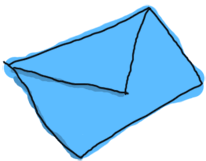
\includegraphics[width=1\linewidth]{envelope.png}
\end{wrapfigure}
Итак, мы определили Erlang как функциональный язык программирования, но в нём также есть большой уклон в параллелизм и высокую надёжность.
Для того, чтобы иметь возможность одновременно выполнять десятки задач, Erlang использует актор\--модель, где каждый актор \--- это отдельный процесс виртуальной машины.
В двух словах, если бы вы были актором в мире Erlang, быть вам одиноким человеком, который сидит в тёмной комнате без окон рядом с почтовым ящиком и ожидает сообщений.
На полученное сообщение вы реагируете следующим образом: если вам пришёл счёт \--- вы его оплачиваете, если пришло поздравление с днём рождения \--- вы выражаете в письме благодарность, а все письма, которые вам непонятны, вы игнорируете.

Актор\--модель в Erlang можно представить как мир, где каждый сидит в своей комнатке и может исполнять несколько определённых задач.
Любое общение происходит только посредством почтовой переписки.
Скучноватая жизнь (и золотая эра для почтовых служб), но благодаря этому вы можете попросить нескольких людей выполнить для вас строго определённый набор задач, и никто не выполнит свою задачу неверно, не сделает ошибку, которая окажет воздействие на работу других людей.
Они даже не будут предполагать о существовании кого\--то ещё, кроме вас (и это прекрасно).

Но не будем заходить с аналогией слишком далеко.
Можно сказать, что Erlang заставляет вас писать акторы (процессы), которые не разделяют информацию с другими частями кода, кроме случаев, когда они посылают друг другу сообщения.
Каждая коммуникация происходит явно, она безопасна и её можно отследить.
Когда мы определяли, что же представляет собой Erlang, то делали это на языковом уровне.
Но это ещё не всё: Erlang в целом является ещё и средой разработки.
Код компилируется в байт\--код и исполняется виртуальной машиной.
Поэтому Erlang, как и Java, может исполняться где угодно.
Стандартный дистрибутив включает (кроме прочего) средства разработки (компилятор, отладчик, профайлер, библиотека для unit\--тестирования), фреймворк Open Telecom Platform (OTP), веб\--сервер, парсер и базу данных mnesia \--- систему хранения пар ключ\--значение, которая способна реплицироваться на несколько серверов, поддерживает вложенные транзакции и позволяет хранить любые данные, которые определены в Erlang.

Виртуальная машина и библиотеки также позволяют обновлять код на работающей системе, не прерывая исполнение, легко распределять код на несколько компьютеров и осуществляет простую, но эффективную обработку ошибок.

\begin{wrapfigure}{r}{0.3\linewidth}
    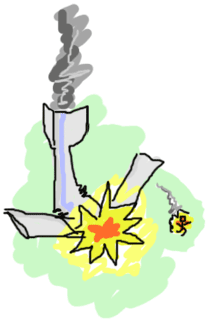
\includegraphics[width=1\linewidth]{letitcrash.png}
\end{wrapfigure}
Позже мы увидим как использовать эти инструменты, но сейчас я расскажу ещё об одном общем правиле Erlang: пусть процесс падает.
Но пусть он падает не как самолёт в авиакатастрофе с десятками человеческих жертв, а пусть падает как канатоходец, под которым натянута страховочная сеть.
Избегать ошибок, конечно же, нужно, но делать проверки на каждый тип ошибки в большинстве случаев нет необходимости.

Итак, Erlang умеет восстанавливаться после ошибок, организовывать код при помощи акторов, производить распределённое масштабирование и обеспечивать параллелизм.
Но это приводит нас к следующему разделу\ldots

\section{Не забывайтесь}
В книге будет много маленьких жёлто\--оранжевых разделов, с названиями похожими на это (их легко заметить).
Erlang в данный момент набирает популярность во многом благодаря пылким речам, которые могут ввести людей в заблуждение.
Могут убедить, что Erlang \--- нечто большее, чем есть на самом деле.
Эти напоминания помогут вам не забываться, если вы переполнены энтузиазмом сверх меры.

Первый случай такого заблуждения относится к мощным возможностям масштабирования, которые заложены в Erlang и осуществляются при помощи лёгких процессов.
Да, действительно, процессы в Erlang очень легки: единовременно могут существовать сотни тысяч таких процессов, но это не означает, что они должны существовать просто потому, что есть такая возможность.
К примеру, вы создаёте игру\--стрелялку.
Было бы безумием представлять все объекты в игре, включая пули, при помощи акторов.
В такой игре вы сможете выстрелить только себе в ногу.
Пересылка сообщений от акторa к актору всё\--таки отнимает ресурсы, как бы малы они ни были.
Если будете дробить задачи слишком сильно, \emph{всё может сильно замедлиться}!

Я расскажу об этом подробнее, когда мы погрузимся в изучение достаточно глубоко, чтобы это нас начало беспокоить.
Но пока что имейте в виду, что бездумно использовать параллелизм при решении проблемы совсем недостаточно для того, чтобы решение стало быстрым.
Не огорчайтесь!
Будут и случаи, когда использовать сотни процессов можно и нужно!
Просто не каждый случай \--- тот самый.

\begin{wrapfigure}{l}{0.3\linewidth}
    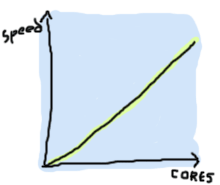
\includegraphics[width=1\linewidth]{scaling.png}
\end{wrapfigure}
Ещё об Erlang говорят, что он может масштабироваться прямо пропорционально количеству вычислительных ядер, которые есть в вашем компьютере, но обычно это не так.
Возможность такая имеется, но большинство задач не получится запустить таким образом, чтобы всё исполнялось одновременно.

Стоит помнить ещё об одном: хотя Erlang и делает некоторые вещи очень хорошо, всё\--таки технически возможно получить те же результаты при помощи других языков.
Верно также и обратное.
Тщательно оценивайте проблему и выбирайте правильный инструмент, исходя из той задачи, которую вы пытаетесь решить.
Erlang \--- не панацея и будет особенно плох в обработке изображений и сигналов или в качестве языка для написания драйверов.
Однако он будет блистать в области большого программного обеспечения для серверов (например: очереди, map\--reduce), в вычислениях совместно с другими языками, в высокоуровневой реализации протоколов и т.д.
Всё, что находится между этими полюсами, зависит лишь от вас.
Не обязательно ограничивать себя только серверными вычислениями на Erlang.
Были случаи, когда люди делали неожиданные и удивительные вещи.
Один из примеров это IANO \--- робот, созданный командой UNICT.
Они используют Erlang для реализации искусственного интеллекта и получили серебрянную медаль на соревновании eurobot в 2009 году.
Ещё один пример \--- Wings 3D.
Платформонезависимая программа трёхмерного моделирования (без рендерера) с открытым исходным кодом, которая написана на Erlang.

\section{Что нужно для изучения}
Для начала вам понадобится лишь текстовый редактор и среда Erlang.
Можно загрузить исходный код и сборки для Windows с официального сайта Erlang.
Не буду углубляться в детали установки, но для Windows достаточно скачать и запустить исполняемый файл.
Не забудьте добавить директорию Erlang в переменную окружения PATH, чтобы получить доступ к ней из командной строки.

В Debian\--подобных Linux дистрибутивах необходимо установить пакет командой \ops{\# apt-get install erlang}.
В Fedora (если установлен <<yum>>), можно проделать то же самое, набрав \ops{\# yum install erlang}.
Однако, официальные репозитории обычно содержат устаревшие версии пакетов Erlang.
Если вы будете использовать старую версию пакета, это может привести к расхождениям между вашим результатом и этим руководством.
К тому же, в некоторых приложениях производительность будет снижена.
Поэтому я рекомендую вам компилировать всё из исходного кода.
Изучите содержимое файла README, который поставляется с пакетом, воспользуйтесь Google для получения подробностей установки, у них это получится намного лучше, чем у меня.

В FreeBSD существует много способов установки.
Если вы используете \ops{postmaster}, можно исполнить команду\\ 
\ops{postmaster lang/erlang}.\\ 
Для установки из портов вопользуйтесь командой\\ 
\ops{cd /usr/ports/lang/erlang;make install clean}.\\ 
И, наконец, если хотите воспользоваться системой пакетов, запустите\\  
\ops{pkg\_add -rv erlang}.\\ 
Если вы пользователь OSX, то можете установить Erlang командой\\ 
\ops{brew install erlang}\\ 
при помощи Homebrew или воспользуйтесь\\ 
\ops{port install erlang}, если предпочитаете MacPorts.\\ 
\colorbox{lgray}
{
\begin{minipage}{1.0\linewidth}
\textbf{Замечание:} на момент написания я использую Erlang версии R13B+, поэтому для наилучших результатов используйте такую же версию, либо более новую.
\end{minipage}
}
\section{Где искать помощь}
Есть несколько мест, где вам помогут.
Хорошую техническую документацию можно найти в man страницах, если вы используете Linux.
Например, в Erlang есть модуль lists (который мы скоро увидим): чтобы получить документацию по этому модулю напишите в консоли \ops{\$ erl -man lists}.

Инсталляция в Windows должна содержать документацию в формате HTML.
Её всегда можно скачать с \href{http://erlang.org/doc/}{официального сайта Erlang} или обратиться к одному из \href{http://erldocs.com}{альтернативных сайтов}.

Как только почувствуете, что пишете что\--то не то, обратитесь к правилам оформления кода, которые можно найти \href{http://www.erlang.se/doc/programming_rules.shtml}{здесь}.
Код в этой книге будет стараться придерживаться этих правил.

Бывают случаи, когда простого понимания технических деталей недостаточно.
Когда наступает такой момент, я обращаюсь к двум источникам знаний: официальной \href{http://www.erlang.org/static/doc/mailinglist.html}{почтовой рассылке} (там есть чему поучиться) и irc каналу \#erlang на irc.freenode.net.

А если вы любите готовые рецепты, то \href{http://trapexit.org}{trapexit} это то что вам нужно.
Ещё они держат зеркало почтовой рассылки в виде форума и общую вики.
Там всегда можно найти что\--нибудь полезное.

\chapter{Начинаем}
\section{Оболочка}
В Erlang можно проверить большую часть кода в эмуляторе.
В нём можно запускать компилированные скрипты, но также можно редактировать код вживую.
Чтобы запустить оболочку в Linux, откройте терминал и наберите \ops{\$ erl}.
Если вы всё правильно настроили, появится текст похожий на этот: 
\begin{lstlisting}[style=repl]
Erlang R13B01 (erts-5.7.2) [source] [smp:2:2] 
[rq:2] [async-threads:0] [hipe] [kernel-poll:false] 
 
Eshell V5.7.2  (abort with ^G) 
\end{lstlisting}

Поздравляю, вы запустили оболочку Erlang! 

Пользователи Windows тоже могут запустить \ops{erl.exe}, но лучше использовать \ops{werl.exe}, который можно найти в стартовом меню (\ops{programs > Erlang}).
Werl это оболочка Erlang, которая создана специально для Windows.
Она поддерживает оформление окон с полосами прокрутки и операциями редактирования (такими, например, как копирование\--вставка, которых очень не хватает в стандартной оболочке \ops{cmd.exe} для Windows).
Правда, если вы захотите использовать перенаправление стандартного ввода\--вывода или каналы, то erl вам всё\--таки пригодится. 

В оболочке мы сможем вводить и запускать код, но сначала посмотрим как с ней обращаться.
\section{Команды оболочки}
В оболочку Erlang встроено подмножество функций популярного текстового редактора Emacs, использование которого берёт начало в 70\--х годах.
Если вы знакомы с Emacs, то ваших знаний будет достаточно.
У всех остальных и без этих знаний всё получится.

\begin{wrapfigure}{r}{0.3\linewidth}
    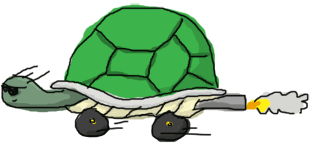
\includegraphics[width=1\linewidth]{shell.png}
\end{wrapfigure}
К примеру, если напечатать какой\--либо текст и нажать \ops{\textasciicircum A}(Ctrl+A), ваш курсор переместится в начало строки.
\ops{\textasciicircum E}(Ctrl+E) переносит курсор в конец строки.
Чтобы перемещаться вперёд и назад, используйте клавиши со стрелками <<влево>> и <<вправо>>.
Клавиши <<вверх>> и <<вниз>> воспроизводят предыдущие или последующие строки, которые уже вводились ранее. Это позволяет не набирать их повторно.

Если написать, к примеру, \ops{li} и нажать <<tab>>, оболочка дополнит за вас слово до \ops{lists:}.
Если нажать tab ещё раз, то оболочка предложит функции, которые могут следовать за lists:.
Так Erlang дополняет имя модуля lists и предлагает функции, которые тот содержит.
Способ записи может показаться странным, но не переживайте, вы к нему быстро привыкнете.
Думаю, мы достаточно ознакомились с функциональностью оболочки, чтобы понимать что к чему.
Кроме одного момента: мы не знаем как из неё выйти!
Ответ на этот вопрос получить очень просто.
Напишите \ops{help().} и вы получите описание команд, которые можно использовать в оболочке (не забудьте написать точку (\ops{\strut.}), она нужна для исполнения команды).
Некоторыми из них мы воспользуемся чуть позже, а сейчас единственная строка, которая нам нужна для того, чтобы выйти из оболочки это:\\ 
\ops{q() -- quit - shorthand for init:stop()} 

Это один из способов выхода (если быть точным, то два способа).
Но от этой команды мало толку, если оболочка зависла!
Если вы внимательно следили за тем, что пишет оболочка при запуске, то видели комментарий о том, что можно <<прекратить исполнение при помощи \ops{\textasciicircum G}>>.
Нажмём это сочетание клавиш и напечатаем h, чтобы получить подсказку.
\begin{lstlisting}[style=repl]
User switch command
--> h
c [nn]            - connect to job
i [nn]            - interrupt job
k [nn]            - kill job
j                 - list all jobs
s [shell]         - start local shell
r [node [shell]]  - start remote shell
q        - quit erlang
? | h             - this message
-->
\end{lstlisting}

Если нажать \ops{i} и следом \ops{c}, то Erlang остановит исполнение кода и возвратится в интерактивную оболочку.
По нажатию \ops{j} будет выведен список запущенных процессов (звёздочка следом за номером указывает, что задача исполняется в данный момент).
Процесс можно прервать, написав \ops{i} и следом номер задачи.
Команда \ops{k} не прерывает оболочку, а полностью завершает её исполнение.
Команда \ops{s} запускает новую оболочку.
\begin{lstlisting}[style=repl]
Eshell V5.7.2  (abort with ^G)
1> "OH NO THIS SHELL IS UNRESPONSIVE!!! *hits ctrl+G*"
User switch command
--> k
--> c
Unknown job
--> s
--> j
2* {shell,start,[]}
--> c 2
Eshell V5.7.2  (abort with ^G)
1> "YESS!"
\end{lstlisting}

Если вы полностью прочитали текст подсказки, то, возможно, заметили, что мы можем запустить удалённую оболочку.
Не буду сейчас вдаваться в детали, но этот факт даёт представление о том, на что ещё способна виртуальная машина Erlang, кроме запуска кода.
А теперь начнём (на этот раз по\--настоящему).

\chapter{Начинаем (по\--настоящему)}
\label{starting-out-for-real}
\setlength{\parindent}{0cm}
\colorbox{lgray}
{
    \begin{minipage}{\linewidth}
    Erlang довольно простой и компактный язык (в том же смысле, в котором C проще чем C++).
    В языке определены несколько фундаментальных типов данных.
    В этой главе мы рассмотрим их большую часть.
    Рекомендуется обязательно прочитать главу, так как в ней объясняются элементы, необходимые для построения всех программ, которые вы позже напишете на Erlang.
    \end{minipage}
}
\setlength{\parindent}{1cm}
\section{Числа}
\label{numbers}
В оболочке Erlang выражения должны завершаться точкой, за которой следует пробел (возврат каретки, пробел и т.д.), иначе это выражение не будет выполнено.
Можно разделять выражения запятыми, но лишь результат последнего выражения отобразится на экране (однако, все остальные выражения будут всё равно исполнены).
Для большинства людей этот синтаксис покажется довольно непривычным.
Он восходит к тем временам, когда Erlang был реализован на Prolog \--- языке логического программирования.

Откройте оболочку Erlang так, как мы это делали в предыдущей главе, и давайте\--ка что\--нибудь попечатаем!
\begin{lstlisting}[style=repl]
1> 2 + 15.
17
2> 49 * 100.
4900
3> 1892 - 1472.
420
4> 5 / 2.
2.5
5> 5 div 2.
2
6> 5 rem 2.
1
\end{lstlisting}

Возможно вы заметили, что для Erlang не имеет значения, вводите вы дробные числа или целые: в арифметических операциях поддерживаются оба типа.
Целые и дробные значения это, в общем\--то, единственные типы данных, которые будут прозрачно обрабатываться математическими операторами Erlang.
Однако, если вы хотите делить целое на целое \--- используйте \ops{div}, а для операции взятия остатка по модулю используйте оператор \ops{rem}(remainder, остаток).

Обратите внимание, что мы можем использовать несколько операторов в одном выражении, и порядок вычисления арифметических операций подчиняется обычным правилам.
\begin{lstlisting}[style=repl]
7> (50 * 100) - 4999.
1
8> -(50 * 100 - 4999).
-1
9> -50 * (100 - 4999).
244950
\end{lstlisting}

Если хотите выразить целое число в системе счисления с основанием отличным от 10, то просто введите его в виде \ops{Основание\#Число} (основание может меняться в диапазоне 2\ldots36):
\begin{lstlisting}[style=repl]
10> 2#101010.
42
11> 8#0677.
447
12> 16#AE.
174
\end{lstlisting}

Прекрасно!
Erlang обладает возможностями калькулятора, который пылится где\--то в дальнем углу вашего стола.
Вдобавок, у калькулятора весьма странный синтаксис!
Просто великолепно!
\section{Неизменные переменные}
\label{invariable-variables}
Арифметические вычисления это отлично, но без возможности сохранять промежуточные результаты далеко не уедешь.
Для этого мы будем использовать переменные.
Если вы прочитали введение к этой книге, то знаете, что переменные в функциональном программировании не могут меняться.
Общее поведение переменных можно продемонстрировать в следующих 7 выражениях (обратите внимание, что имена переменных начинаются с заглавной буквы):
\begin{lstlisting}[style=repl]
1> One.
* 1: variable 'One' is unbound
2> One = 1.
1
3> Un = Uno = One = 1.
1
4> Two = One + One.
2
5> Two = 2.
2
6> Two = Two + 1.
** exception error: no match of right hand side value 3
7> two = 2.
** exception error: no match of right hand side value 2
\end{lstlisting}

Первое, что можно заметить: значение можно присваивать переменной ровно один раз, после этого можно <<притвориться>>, что вы присваиваете значение, только если это то же самое значение, которое ей уже присвоено.
Erlang\--у не понравится, если они будут различны.
Объяснение кроется в свойствах оператора \ops{\strut=}.
Оператор \ops{\strut=} (не переменные) выполняет функцию сравнения значений и сообщает, если они различаются.
Если они одинаковы, то оператор просто возвращает само значение:
\begin{lstlisting}[style=repl]
8> 47 = 45 + 2.
47
9> 47 = 45 + 3.
** exception error: no match of right hand side value 48
\end{lstlisting}

Оператор в сочетании с переменными делает следующее: если выражение слева \--- свободная переменная (с ней не связано значение), Erlang автоматически свяжет значение, которое находится справа, с переменной слева.
После этого сравнение завершится успешно, и значение переменной сохранится в памяти.

Такое поведение оператора \ops{\strut=} это основа <<сопоставления с образцом>> (pattern matching), которое существует во многих функциональных языках программирования, хотя его реализация в Erlang обычно считается более гибкой и полной в сравнении с аналогами.
Мы рассмотрим сопоставление с образцом более детально, когда будем разбираться с кортежами и списковыми типами, чуть позже в этой же главе, а также в связи с функциями в последующих главах.

Ещё один факт, который можно почерпнуть из команд 1\--7: имена переменных должны начинаться с заглавной буквы.
Команда 7 завершилась ошибкой, потому что слово \emph{two} начинается со строчной буквы.
Формально имена переменных  могут начинатся со знака подчёркивания ('\_'), но по соглашению такие имена используются только для переменных, значение которых вас не интересует, но вы всё\--таки посчитали, что было бы неплохо описать, что же в них содержится.

Ещё можно завести переменную, имя которой будет состоять просто из знака подчёркивания:
\begin{lstlisting}[style=repl]
10> _ = 14+3.
17
11> _.
* 1: variable '_' is unbound
\end{lstlisting}

В отличие от любой другой переменной, у этой никогда не будет собственного значения.
На данный момент это для нас абсолютно бесполезно, но запомним, что такая переменная существует.
Она нам ещё пригодится.\\ 
\colorbox{lgray}
{
\begin{minipage}{1.0\linewidth}
\textbf{Замечание:} если вы экспериментируете в оболочке и присвоили переменной неверное значение, то можно <<удалить>> эту переменную при помощи функции \ops{f(Variable).}.
Чтобы очистить все переменные, используйте \ops{f().}.
\par 
Эти функции работают только в оболочке и созданы специально, чтобы помогать вам во время тестирования.
В настоящих программах удалять значения таким способом мы не сможем.
Смысл этого поведения становится понятен, если представить Erlang в производственном окружении: вполне возможно, что оболочка будет непрерывно запущена на протяжении нескольких лет\ldots Готов поспорить, что переменная X будет использована за это время больше одного раза.
\end{minipage}
}
\section{Атомы}
\label{atoms}
Существует причина, по которой имена переменных должны начинаться с заглавной буквы, и причина эта \--- атомы.
Атомы это литералы: константы, значением которых является их собственное имя.
Что видите, то и получаете, больше рассчитывать не на что.
Атом \emph{cat} просто означает <<cat>> и ничего больше.
С ним нельзя поиграть, его нельзя изменить, его нельзя разбить вдребезги; это \emph{cat}.
Cмиритесь с этим.

Хотя запись атомов в виде слов, которые начинаются со строчной буквы, и считается предпочтительной, записывать их можно и другими способами:
\begin{lstlisting}[style=repl]
1> atom.
atom
2> atoms_rule.
atoms_rule
3> atoms_rule@erlang.
atoms_rule@erlang
4> 'Atoms can be cheated!'.
'Atoms can be cheated!'
5> atom = 'atom'.
atom
\end{lstlisting}

Если атом не начинается со строчной буквы или содержит символы отличные от букв и цифр, знака подчёркивания (\_) или @, то он должен обрамляться одиночными кавычками (').
Выражение под номером 5 также показывает, что атом, заключённый в одиночные кавычки, это совершенно то же самое, что и атом без них.

\begin{wrapfigure}{l}{0.3\linewidth}
    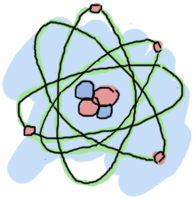
\includegraphics[width=1\linewidth]{atom.png}
\end{wrapfigure}
Я сравнил атомы с константами, у которых значением является их собственное имя.
Вы, быть может, раньше работали с кодом, в котором использовались константы.
Пусть, к примеру, у меня есть значения, которые соответствуют цвету глаз: \ops{BLUE -> 1, BROWN -> 2,} \ops{GREEN -> 3, OTHER -> 4}.
Необходимо сопоставить имя константы с некоторым значением.
Атомы позволяют без этого обойтись.
Цвет глаз может просто быть 'blue', 'brown', 'green' и 'other'.
Эти цвета можно использовать в коде где угодно: значения никогда не будут пересекаться, и, вдобавок, такая константа всегда инициализирована.
Если вам и в самом деле нужны именно константы со связанными значениями, то всё\--таки существует способ их заполучить.
Мы рассмотрим его в главе~\ref{modules}.

Таким образом, атом хорош для оценки и представления данных, которые к нему прикреплены.
Без данных найти ему достойное применение сложновато.
Довольно об атомах.
Их время настанет, когда мы сможем компоновать с ними другие типы данных.
\\ 
\colorbox{lorange}
{
    \begin{minipage}{1.0\linewidth}
\textbf{Не забывайтесь:}

Атомы прекрасно подходят для отсылки сообщений и представления констант, но во многих случаях использование атомов скрывает подвох.
Обращение к атому происходит через <<таблицу атомов>>, которая занимает память (4 байта/атом в 32\--битной системе, 8 байт/атом в 64\--битной системе).
Таблица атомов не обрабатывается сборщиком мусора, а поэтому атомы будут накапливаться до тех пор, пока система не остановится из\--за нехватки памяти, либо потому что было определено максимальное количество атомов \--- 1048577.

Поэтому атомы нельзя генерировать динамически ни в коем случае.
Если ваша система должна быть надёжной, но ввод пользовательских данных позволяет кому\--либо ронять её по желанию, то у вас серьёзные проблемы.
Атомы необходимо рассматривать только как инструменты разработчика, потому что на самом деле они как раз ими и являются.
\end{minipage}
}
\colorbox{lgray}{
    \begin{minipage}{1.0\linewidth}
    \textbf{Замечание:} некоторые атомы являются зарезервированными словами и их нужно использовать так, как было задумано разработчиками языка: для обозначения имён функций, операторов, выражений и т.д.
    Вот эти атомы: \ops{after and andalso band begin}
\ops{bnot bor bsl bsr bxor case catch}
\ops{cond div end fun if let not of}
\ops{or orelse query receive rem try when xor}
\end{minipage}
}
\section{Булева алгебра и операторы сравнения}
\label{boolean-algebra-comparison-operators}
\begin{wrapfigure}[7]{r}{0.20\linewidth}
    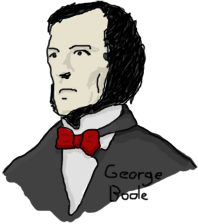
\includegraphics[width=1.0\linewidth]{boole.png}
\end{wrapfigure}
Если бы человек не мог отличать большое от малого, истину от лжи, то ему бы пришлось нелегко.
В Erlang, как и в любом другом языке, есть возможность применения булевых операций и сравнения элементов.
Булева алгебра очень проста:\\ 
\begin{lstlisting}[style=repl]
1> true and false.
false
2> false or true.
true
3> true xor false.
true
4> not false.
true
5> not (true and true).
false
\end{lstlisting} 
\colorbox{lgray}
{
    \begin{minipage}{1.0\linewidth}
        \textbf{Замечание:} Операторы \ops{and} и \ops{or} всегда вычисляют аргументы, находящиеся по обе стороны от оператора.
        Если вам нужны операторы, которые вычисляют правую сторону только при необходимости, используйте \ops{andalso} и \ops{orelse}.
    \end{minipage}
} 

Проверка на равенство и неравенство тоже выполняется очень просто, но при этом используют несколько другие символы, чем те, которые можно увидеть во многих других языках:
\begin{lstlisting}[style=repl]
6> 5 =:= 5.
true
7> 1 =:= 0.
false
8> 1 =/= 0.
true
9> 5 =:= 5.0.
false
10> 5 == 5.0.
true
11> 5 /= 5.0.
false
\end{lstlisting}

Во\--первых, если в привычном языке для проверки на равенство и неравенство используется \ops{==} и \ops{!=}, то в Erlang используется \ops{=:=} и \ops{=/=}.
Три последних выражения (строки с 9 по 11) также знакомят нас с ловушкой: Erlang не делает различий при выполнении арифметических действий между целыми числами и числами с плавающей запятой, но он будет различать эти числа при сравнении.
Впрочем, беспокоиться не о чем, потому что в этом случае на помощь придут операторы \ops{==} и \ops{/=}.
Помните об этом различии, если вам понадобится сравнить числа, не сравнивая их типы.

Остальные операторы сравнения: \ops{$<$} (меньше чем), \ops{$>$} (больше чем), \ops{$>=$} (больше либо равно) и \ops{$=<$} (меньше либо равно).
Мне кажется, что последний оператор записывается задом\--наперёд, и из\--за него в моём коде часто появляются синтаксические ошибки.
Будьте внимательны с этим \ops{$=<$}.
\begin{lstlisting}[style=repl]
12> 1 < 2.
true
13> 1 < 1.
false
14> 1 >= 1.
true
15> 1 =< 1.
true
\end{lstlisting}

Как узнать что произойдёт, если выполнить \ops{5 + llama} или \ops{5 == true}?
Нет способа лучше, чем исполнить эти выражения и испугаться сообщений об ошибках!
\begin{lstlisting}[style=repl]
12> 5 + llama.
** exception error: bad argument in an arithmetic expression
    in operator  +/2
        called as 5 + llama
\end{lstlisting}

Ну, что сказать?
Erlang не нравится, что вы неправильно используете его базовые типы!
Здесь эмулятор возвращает вполне понятное сообщение об ошибке.
Он сообщает, что ему не по нраву один из аргументов, которые окружают оператор \ops{+}!

Впрочем, Erlang не всегда сходит с ума из\--за неверных типов:
\begin{lstlisting}[style=repl]
13> 5 =:= true.
false
\end{lstlisting}

Почему для некоторых операторов различие в типах не существено, а для других имеет значение?
Хотя Erlang не разрешает суммировать что попало с чем угодно, он позволяет \emph{сравнивать}.
Так вышло потому, что создатели Erlang поставили прагматизм выше теории и решили, что было бы неплохо иметь возможность писать, к примеру, общие алгоритмы сортировки, которые могли бы упорядочивать любые элементы.
В большинстве случаев это упрощает жизнь.

Когда работаете с булевой алгеброй и сравнениями, стоит помнить ещё об одной вещи:
\begin{lstlisting}[style=repl]
14> 0 == false.
false
15> 1 < false.
true
\end{lstlisting}

Если вы раньше имели дело преимущественно с процедурными или объектно\--ориентированными языками, то, вероятно, сейчас рвёте волосы на голове.
Строка 14 должна возвращать \emph{true}, а строка 15 \emph{false}!
Везде false означает 0, а true \--- всё остальное!
Но не в Erlang.
Потому что я вам солгал.
Да, я вам наврал.
Стыд мне и позор.

В Erlang нет такого понятия как булевы значения \emph{true} и \emph{false}.
Элементы true и false на самом деле являются атомами, но они хорошо интегрированы в язык, и проблем с ними не будет, пока вы считаете, что false и true \--- это просто false и true, и ничего больше.\\ 
\colorbox{lgray}
{
    \begin{minipage}{1.0\linewidth}
    \textbf{Замечание:} при сравнении элементы выстраиваются в следующем порядке:\\ 
    \ops{number < atom < reference < fun < port < pid < tuple < list < bit string} 
    
    Все эти понятия вам пока неизвестны, но вы будете с ними знакомиться по мере продвижения по тексту книги.
    Просто помните, что именно благодаря им вы можете сравнивать что угодно с чем угодно!
    Процитирую Joe Armstrong, одного из создателей Erlang: <<Важен не сам порядок, а то, что этот порядок чётко определён.>>
    \end{minipage}
}
\section{Кортежи}
\label{tuples}
Кортеж \--- это способ организации данных.
С его помощью можно сгруппировать элементы, когда вам известно их количество.
Кортежи в Erlang записываются следующим образом: \ops{\{Element1, Element2,\ldots, ElementN\}}.
Как пример можно привести координаты (x, y), которые задают положение точки на плоскости.
Мы можем представить координаты как кортеж двух элементов:
\begin{lstlisting}[style=repl]
1> X = 10, Y = 4.
4
2> Point = {X,Y}.
{10,4}
\end{lstlisting}

В этом случае точка будет всегда представлена двумя значениями.
Вместо того, чтобы повсюду таскать за собой переменные X и Y, можно определить всего одну.
Но что же делать, если у меня есть переменная\--точка, а мне необходима лишь её X координата?
Эту информацию можно легко получить.
Помните, когда мы присваивали значения переменным, Erlang не возражал, если присваиваемые значения были равны содержимому переменных.
Давайте это используем!
Возможно, вам понадобится очистить командой \ops{f()} переменные, которые мы определили ранее.
\begin{lstlisting}[style=repl]
3> Point = {4,5}.
{4,5}
4> {X,Y} = Point.
{4,5}
5> X.
4
6> {X,_} = Point.
{4,5}
\end{lstlisting}
\begin{wrapfigure}{l}{0.3\textwidth}
    
\includegraphics[width=1.0\linewidth]{mr-brackets.png}
\end{wrapfigure}

Теперь для получения первого значения в кортеже, мы можем использовать \emph{X}!
Как так получилось?
Сначала у \emph{X} и \emph{Y} значений не было, и они считались свободными переменными.
Мы поместили их в кортеж \emph{\{X, Y\}} по левую сторону оператора \ops{=}.
Оператор \ops{=} сравнивает между собой \emph{\{X, Y\}} и \emph{\{4, 5\}}.
У Erlang хватает сообразительности, чтобы распаковать значения в кортеже и распределить их по свободным переменным слева от оператора присваивания.
После этого сравнение приходит к виду \ops{\{4, 5\} = \{4, 5\}}, и, очевидно, завершается успехом!
Это одна из многих форм операции сопоставления с образцом (pattern matching).

Заметьте, что в шестом выражении я использовал анонимную переменную \_.
Она должна использоваться именно в таких случаях: когда необходимо отбросить значение, которое нам не понадобится.
Переменная \_ всегда определена как свободная и служит универсальным элементом подстановки (wildcard) для сопоставления с образцом.
Сопоставление с образцом для распаковки кортежей будет работать только когда количество элементов (длина кортежа) одинаково с обеих сторон.
\begin{lstlisting}[style=repl]
7> {_,_} = {4,5}.
{4,5}
8> {_,_} = {4,5,6}.
** exception error: no match of right hand side value {4,5,6}
\end{lstlisting}

Кортежи полезны и при работе с одиночными значениями.
Простейший пример, температура:
\begin{lstlisting}[style=repl]
9> Temperature = 23.213.
23.213
\end{lstlisting}

В такой денёк неплохо было бы пойти на пляж\ldots Погодите\--ка, это температура по шкале Кельвина, Цельсия или Фаренгейта?
\begin{lstlisting}[style=repl]
10> PreciseTemperature = {celsius, 23.213}.
{celsius,23.213}
11> {kelvin, T} = PreciseTemperature.
** exception error: no match of right hand side value {celsius,23.213}
\end{lstlisting}

Операция вызывает ошибку, но это как раз то, что нам необходимо! Мы снова наблюдаем в работе сопоставление с образцом.
Оператор \ops{=} сравнивает \emph{\{kelvin, T\}} и \emph{\{celsius, 23.213\}}.
Несмотря на то, что переменная T свободна, Erlang при сравнении не посчитает атом \emph{celsius} идентичным атому \emph{kelvin}.
Будет брошено исключение, которое остановит выполнение кода.
Та часть нашей программы, которая ожидает температуру по шкале Кельвина, не сможет обработать значение, которое будет представлено в градусах Цельсия.
Это трюк облегчает отладку кода и даёт программисту представление о передаваемых данных.
Кортеж, который содержит атом, а следом за ним одиночный элемент \--- называется <<меченым кортежем>>.
Все элементы кортежа могут принадлежать к разным типам данных, и элементами кортежа могут быть и другие кортежи: \begin{lstlisting}[style=repl]
12> {point, {X,Y}}.
{point,{4,5}}
\end{lstlisting}

Что же делать, когда необходимо работать с несколькими точками?
\section{Списки!}
\label{lists}
Списки \--- это хлеб насущный для многих функциональных языков.
Их используют для решения множества задач, и они, несомненно, являются наиболее используемой структурой данных в Erlang.
Списки могут содержать всё что угодно!
Числа, атомы, кортежи, другие списки \--- всё что пожелаете в одной структуре.
Основной способ записи для списков: \ops{[Element1, Element2,\ldots,ElementN]}, и в них можно смешивать несколько разных типов данных:
\begin{lstlisting}[style=repl]
1> [1, 2, 3, {numbers,[4,5,6]}, 5.34, atom].
[1,2,3,{numbers,[4,5,6]},5.34,atom]
\end{lstlisting}

Всё просто, не так ли?
\begin{lstlisting}[style=repl]
2> [97, 98, 99].
"abc"
\end{lstlisting}

Ой\--ой!
Вот одна из тех вещей в Erlang, которая многим не нравится: строки!
Строки \--- тоже списки, поэтому записываются они совершенно так же!
Почему же люди их не любят?
А вот почему:
\begin{lstlisting}[style=repl]
3> [97,98,99,4,5,6].
[97,98,99,4,5,6]
4> [233].
"é"
\end{lstlisting}

Erlang напечатает список чисел в числовом представлении, только если хотя бы одно из них невозможно представить в виде буквы!
Настоящих строк в Erlang просто нет!
Вы ещё не раз встретитесь с этой особенностью, и из\--за неё временами будете ненавидеть язык.
Но не отчаивайтесь \--- есть и другие способы записи строк.
C ними мы познакомимся чуть позже в этой главе.\\ 
\colorbox{lorange}
{
    \begin{minipage}{1.0\linewidth}
        \textbf{Не забывайтесь:}\\ 
        Возможно, вы слышали, что Erlang плохо подходит для работы со строками, потому что, в отличие от большинства других языков, в нём нет встроенных строк.
        Так вышло потому, что Erlang был создан и использовался в телекоммуникационных компаниях.
        Они никогда (или редко) не использовали строки, и поэтому им просто не приходило в голову официально добавить их в язык.
        Тем не менее, недостатки Erlang в области строковых преобразований со временем устраняются.
        Виртуальная машина имеет встроенную поддержку Unicode\--строк, и в целом операции со строками постоянно ускоряются.
        
        Строки также можно хранить в виде двоичной структуры данных, что увеличивает эффективность хранения и скорость обработки.
        Но всё же в стандартной библиотеке не хватает некоторых функций.
        Не вызывает сомнений тот факт, что в Erlang можно работать со строками, но для решения задач, в которых нужно делать много строковых преобразований, лучше подходят другие языки, например Perl или Python.
    \end{minipage}
}

Для склейки списков используют оператор\ops{++}.
Противоположное действие выполняет оператор \ops{$--$}, который удаляет элементы из списка:
\begin{lstlisting}[style=repl]
5> [1,2,3] ++ [4,5].
[1,2,3,4,5]
6> [1,2,3,4,5] -- [1,2,3].
[4,5]
7> [2,4,2] -- [2,4].
[2]
8> [2,4,2] -- [2,4,2].
[]
\end{lstlisting}

Оба оператора, \ops{++} и \ops{$--$} \--- ассоциативны справа.
Это означает, что элементы нескольких последовательных операций \ops{++} и \ops{$--$} будут обрабатываться справа налево, как в следующем примере:
\begin{lstlisting}[style=repl]
9> [1,2,3] -- [1,2] -- [3].
[3]
10> [1,2,3] -- [1,2] -- [2].
[2,3]
\end{lstlisting}

Продолжим.
Первый элемент списка называется Головой (головным элементом), остальные элементы списка называются Хвостом (хвостовыми элементами).
Для их получения будем использовать две встроенные функции:
\begin{lstlisting}[style=repl]
11> hd([1,2,3,4]).
1
12> tl([1,2,3,4]).
[2,3,4]
\end{lstlisting}
\colorbox{lgray}
{
    \begin{minipage}{1.0\linewidth}
        \textbf{Замечание:} встроенными обычно называют функции (ВФ), которые невозможно реализовать на чистом Erlang.
        Поэтому они реализованы на С или любом другом языке, на котором реализован Erlang (в 80\--х это был Prolog).
        Есть также и ВФ, которые можно реализовать на Erlang, но их всё равно пишут на С для ускорения часто используемых операций.
        Как пример можно привести функцию \ops{length(List)}, которая (как вы, наверное, догадались) возвращает длину списка, который был передан ей в качестве аргумента.
    \end{minipage}
}

Операция доступа к головному элементу или добавления к голове списка выполняется быстро и эффективно.
Практически во всех случаях, в которых вы сталкиваетесь со списками, необходимо выполнять операции с головой списка.
Из\--за того, что эта операция используется так часто, существует более простой метод отделения головы от хвоста \--- при помощи сопоставления с образцом: \ops{[Head|Tail]}.
Вот как можно добавить в голову списка новый элемент:
\begin{lstlisting}[style=repl]
13> List = [2,3,4].
[2,3,4]
14> NewList = [1|List].
[1,2,3,4]
\end{lstlisting}

При обработке списка неплохо было бы иметь возможность быстро сохранить хвост, чтобы чуть позже его обработать.
Если вы помните как работают кортежи, и как мы использовали сопоставление с образцом для распаковки координат точки (\emph{\{X, Y\}}), то знайте, что мы можем очень похожим методом извлечь первый элемент (головной).
\begin{lstlisting}[style=repl]
15> [Head|Tail] = NewList.
[1,2,3,4]
16> Head.
1
17> Tail.
[2,3,4]
18> [NewHead|NewTail] = Tail.
[2,3,4]
19> NewHead.
2
\end{lstlisting}

Оператор \ops{|} называется cons\--оператором (конструктором).
Любой список можно построить при помощи cons\--оператора и значений списка:
\begin{lstlisting}[style=repl]
20> [1 | []].
[1]
21> [2 | [1 | []]].
[2,1]
22> [3 | [2 | [1 | []] ] ].
[3,2,1]
\end{lstlisting}

Таким образом, любой список можно построить по следующей формуле: \ops{[Term1| [Term2 | [\ldots | [TermN]]]]\ldots}.
То есть, списки можно определить рекурсивно как заголовок, за которым следует хвост, который, в свою очередь является заголовком, за которым следуют другие заголовки.
В этом смысле можно представить список в виде земляного червя: можно разрубить его пополам, и вот у вас уже два червя.

\begin{figure}[h!]
    \centering
    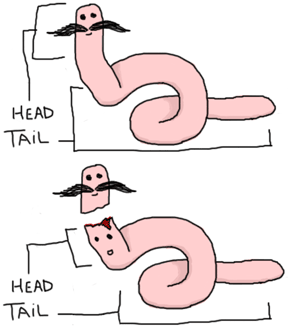
\includegraphics[width=0.5\textwidth]{worm.png}
\end{figure} 

Способ построения списков в Erlang иногда немного озадачивает людей, которые не имели дело с подобными конструкторами.
Чтобы немного привыкнуть к этой записи, попробуйте прочитать следующие примеры (подсказка: все они равнозначны друг другу):\\ 
\begin{lstlisting}[style=repl]
[a, b, c, d]
[a, b, c, d | []]
[a, b | [c, d]]
[a, b | [c | [d]]]
[a | [b | [c | [d]]]]
[a | [b | [c | [d | [] ]]]]
\end{lstlisting}

Если вам понятна эта концепция, то будут понятны и списочные выражения.\\ 
\colorbox{lgray}
{
    \begin{minipage}{1.0\linewidth}
        \emph{Замечание:} при использовании формы \ops{[1 | 2]} мы получаем так называемый <<неправильный список>>.
        Неправильные списки будут работать в сопоставлении с образцом вида \ops{[Head|Tail]}, но стандартные функции Erlang (даже \ops{length()}) с ними работать не будут.
        В этих операциях можно использовать только правильные списки.
        Последним элементом правильных списков всегда является пустой список.
        Когда мы объявляем список таким способом: \ops{[2]}, то автоматически формируется правильный список.
        Поэтому запись \ops{[1|[2]]} сгенерирует правильный список!
        Хотя неправильные списки синтаксически верны, их редко используют где\--то ещё, кроме пользовательских структур данных.
    \end{minipage}
}
\section{Списочные выражения}
\label{list-comprehensions}
Списочные выражения дают возможность формировать или менять списки.
Программы, в которых используются списочные выражения, намного короче и проще для понимания.
Этот способ основан на записи математических множеств; если вы когда\--либо занимались теорией множеств, или сталкивались с математической записью, то наверняка знаете как она работает.
Мы задаём множество через определение свойств, которым должны удовлетворять его элементы.
Сначала списочные выражения могут показаться немного сложными, но усилия, потраченные на их понимание, стоят того.
С их помощью код становится чище и короче, поэтому вводите примеры и пытайтесь их понять!

Приведём пример математической записи множества: $\{x \in 
\mathbb{R}: x = x^2\}$.
Эта запись говорит о том, что вы хотите получить действительные числа, которые равны собственному квадрату.
Результатом будет множество $\{0, 1\}$.
В качестве примера более простой записи можно привести \ops{\{x : x $>$ 0\}}.
В результате мы должны получить все числа больше 0.

Списочные выражения в Erlang можно представить как построение множеств из других множеств.
Пусть нам дано множество \ops{\{2n : n in L\}}, где L \--- список $[1, 2, 3, 4]$.
В Erlang это можно записать как:\\ 
\begin{lstlisting}[style=repl]
1> [2*N || N <- [1,2,3,4]].
[2,4,6,8]
\end{lstlisting}

Если сравнить математическую запись с записью в Erlang, то можно заметить, что они не так уж сильно различаются: фигурные скобки (\{\}) становятся квадратными ([]), двоеточие (:) становится двумя вертикальными чертами (||), а слово <<in>> переходит в символ стрелки ($<-$).
Мы просто заменяем символы на другие, но логика остаётся прежней.
В примере, приведённом выше, каждое значение $[1, 2, 3, 4]$ последовательно помещается в N (проводится операция сопоставления с образцом для каждого значения в списке).
Стрелка выполняет ту же функцию, что и оператор\ops{=}, с тем лишь отличием, что она не бросает исключения.

Также в списочные выражения можно добавлять ограничивающие условия, используя операции, которые возвращают булевы значения.
Если нам понадобились чётные числа от единицы до десяти, мы можем записать что\--то вроде:
\begin{lstlisting}[style=repl]
2> [X || X <- [1,2,3,4,5,6,7,8,9,10], X rem 2 =:= 0].
[2,4,6,8,10]
\end{lstlisting}

Где конструкция \ops{X rem 2 =:= 0} проверяет число на чётность.
Практическая польза этого подхода становится ясна, когда нам нужно применить функцию к каждому элементу списка или наложить на элементы какие\--либо ограничения и т.д.
К примеру, мы владеем рестораном.
Входит посетитель, видит наше меню и спрашивает, может ли он получить цены всех блюд, которые стоят от \$3 до \$10, включая налоги (скажем, 7\%), и налог должен быть применён после сравнения.
\begin{lstlisting}[style=repl]
3> RestaurantMenu = [{steak, 5.99}, {beer, 3.99}, {poutine, 3.50}, {kitten, 20.99}, {water, 0.00}].
[{steak,5.99},
    {beer,3.99},
    {poutine,3.5},
    {kitten,20.99},
{water,0.0}]
4> [{Item, Price*1.07} || {Item, Price} <- RestaurantMenu, Price >= 3, Price =< 10].
[{steak,6.409300000000001},{beer,4.2693},{poutine,3.745}]
\end{lstlisting}

Конечно, неплохо было бы округлить числа для улучшения читаемости, но вы поняли в чём смысл.
Таким образом, списочные выражения в Erlang готовят по следующему рецепту: \ops{NewList = [Expression || Pattern}\\ 
\ops{ $<-$ List, Condition1, Condition2, ... ConditionN]}.
Элемент \ops{Pattern $<-$ List} называется Генератором.
И их может быть несколько!\\ 
\begin{lstlisting}[style=repl]
5> [X+Y || X <- [1,2], Y <- [2,3]].
[3,4,4,5]
\end{lstlisting}

Это выражение выполняет следующие операции: \ops{1 + 2},\ops{1 + 3},\ops{2 + 2},\ops{2 + 3}.
Так что в обобщённом виде вы получите: \ops{NewList = }\\ 
\ops{[Expression || GeneratorExp1, GeneratorExp2, ..., GeneratorExpN,}\\ 
\ops{Condition1, Condition2, ... ConditionM]}.
Обратите внимание, что выражения\--генераторы можно комбинировать с сопоставлением по образцу, и использовать в качестве фильтра:
\begin{lstlisting}[style=repl]
6> Weather = [{toronto, rain}, {montreal, storms}, {london, fog},  
6>            {paris, sun}, {boston, fog}, {vancouver, snow}].
[{toronto,rain},
    {montreal,storms},
    {london,fog},
    {paris,sun},
    {boston,fog},
{vancouver,snow}]
7> FoggyPlaces = [X || {X, fog} <- Weather].
[london,boston]
\end{lstlisting}

Если элемент списка <<Weather>> не совпадает с образцом \{X, fog\}, то в списочном выражении он просто игнорируется, тогда как при использовании с оператором \ops{=} было бы выброшено исключение.

Остался ещё один базовый тип данных, который мы должны рассмотреть.
В Erlang встроена функциональность, которая легко и просто позволяет преобразовывать двоичные данные.
\section{Битовый синтаксис!}
\label{bit-syntax}
Во многих языках есть поддержка манипуляций с числами, атомами, кортежами, списками, записями и/или структурами и т.д.
Но большая часть этих языков содержит очень грубые методы манипулирования двоичными данными.
Erlang старается предоставить полезные абстракции для работы с двоичными данными при помощи усовершенствованного сопоставления с образцом.
Это превращает работу с необработанными двоичными данными в приятное и простое (я не вру) занятие.
Метод был разработан для решения телекоммуникационных задач.
Битовые манипуляции предоставляют уникальный синтаксис и идиомы, которые на первый взгляд могут показаться странными, но обретают смысл, если вы понимаете, как устроены биты и байты.
\textbf{В противном случае вам лучше пропустить остаток этой главы.}

В соответствии с битовым синтаксисом, двоичные данные обрамляются символами $<<$ и $>>$, и их разделяют на читаемые сегменты при помощи запятых.
Сегмент \--- это битовая последовательность в двоичном представлении (не обязательно с выравниванием по границе байта, но такое выравнивание происходит по умолчанию).
Представим, что мы хотим хранить пиксель оранжевого цвета в 24\--битном представлении.
Если вам приходилось когда\--либо сталкиваться с цветовым представлением в Photoshop или в CSS, то запись в формате \#RRGGBB должна быть вам знакома.
Оранжевый оттенок можно записать как \emph{\#F09A29}.
Erlang преобразует эту запись в следующий вид:
\begin{lstlisting}[style=repl]
1> Color = 16#F09A29.
15768105
2> Pixel = <<Color:24>>.
<<240,154,41>>
\end{lstlisting}

Это означает что\--то вроде: <<Расположи двоичное представление числа \emph{\#F09A29} в 24\--х битах (Красный в 8 битах, Зелёный в 8 и Синий тоже в 8 битах) переменной Pixel>>.
Значение можно будет позже взять и в неизменном виде записать в файл.
На первый взгляд ничего особенного в этом нет, но если вы откроете записанный файл в текстовом редакторе, то увидите лишь несколько нечитаемых символов.
Если этот файл считать при помощи Erlang, то его содержимое в двоичном представлении будет снова преобразовано в удобный формат \emph{$<<$240,151,41$>>$}!

Но самое интересное, что для распаковки двоичных данных можно использовать сопоставление с образцом:
\begin{lstlisting}[style=repl]
3> Pixels = <<213,45,132,64,76,32,76,0,0,234,32,15>>.
<<213,45,132,64,76,32,76,0,0,234,32,15>>
4> <<Pix1,Pix2,Pix3,Pix4>> = Pixels.
** exception error: no match of right hand side value <<213,45,132,64,76,32,76,
0,0,234,32,15>>
5> <<Pix1:24, Pix2:24, Pix3:24, Pix4:24>> = Pixels.
<<213,45,132,64,76,32,76,0,0,234,32,15>>
\end{lstlisting}

В 3\--й команде мы определили значение, которое соответствует двоичному представлению 4\--х пикселов в RGB пространстве.
В 4\--м выражении мы попытались распаковать 4 значения из двоичной величины.
После чего было выброшено исключение, так как в исходной величине не 4 сегмента, а 12!
Поэтому мы говорим Erlang, что каждая переменная слева будет содержать 24 бита.
Именно это и означает запись \ops{Var:24}.
Далее мы можем взять первый пиксел и распаковать его в отдельные цветовые компоненты:
\begin{lstlisting}[style=repl]
6> <<R:8, G:8, B:8>> = <<Pix1:24>>.
<<213,45,132>>
7> R.
213
\end{lstlisting}

<<Да, вышло неплохо.
А что если мне нужен лишь первый компонент?
Мне всё равно придётся постоянно распаковывать все значения?>>
Ха!
Прочь сомнения!
Erlang приходит на помощь, предоставляя комбинацию синтаксического сахара и сопоставления с образцом:
\begin{lstlisting}[style=repl]
8> <<R:8, Rest/binary>> = Pixels.
<<213,45,132,64,76,32,76,0,0,234,32,15>>
9> R.
213
\end{lstlisting}

Неплохо, да?
А всё потому что Erlang воспринимает несколько способов описания двоичного сегмента.
Можно использовать все перечисленные ниже:

Value

Value:Size

Value/TypeSpecifierList

Value:Size/TypeSpecifierList

где Size указывает количество бит, а TypeSpecifierList обозначает одно или несколько понятий из следующего списка:

\begin{minipage}{\textwidth}
\textbf{Тип}\\ 
Возможные значения: \ops{integer | float | binary | bytes | bitstring | bits | utf8}\\ 
\ops{| utf16 | utf32}\\  
Так определяется вид используемых двоичных данных.
Заметьте, что 'bytes' это псевдоним для 'binary', а 'bits'\--- для 'bitstring'.
Если тип не задан, то Erlang по умолчанию использует 'integer'.\\ 
\end{minipage}

\begin{minipage}{\textwidth}
    \textbf{Знак}\\ 
    Возможные значения: \ops{signed | unsigned}\\ 
    Имеет значение только при сопоставлении, когда тип \--- integer.
    По умолчанию используется 'unsigned'.\\ 
\end{minipage}

\begin{minipage}{\textwidth}
    \textbf{Порядок байтов}\\ 
    Возможные значения: \ops{big | little | native}\\ 
    Порядок байтов имеет значение, когда задан тип integer, utf16, utf32 или float.
    От порядка зависит то, как система считывает двоичные данные.
    Например, заголовок изображения в формате BMP содержит размер файла в виде 4\--байтного целого числа.
    Пусть размер файла равен 72 байта, тогда little\--endian система представит его в виде \ops{$$<<$$72,0,0,0$$>>$$}, а big\--endian система в виде \ops{$$<<$$0,0,0,72$$>>$$}.
    Первое будет прочитано как '72', а второе как '1207959552', поэтому старайтесь сделать так, чтобы порядок байтов был верным.
    Также существует опция 'native', которая устанавливает порядок байт, используемый процессором.
    По умолчанию используется порядок 'big'.\\ 
\end{minipage}

\begin{minipage}{\textwidth}
    \textbf{Единичный элемент}\\ 
    Записывается как \ops{unit:Integer}\\ 
    Это размер одного сегмента в битах.
    Допустимый диапазон 1..256. По умолчанию равен 1 для integer, float, битовых строк и 8 для двоичных данных.
    Для типов utf8, utf16 и utf32 единичный элемент определять не нужно.
    Произведение Размера на Единичный элемент равно количеству бит, которые занимает сегмент, и должно быть кратным 8.
    Задание размера элемента часто используется для выравнивания по границе байта.\\  
\end{minipage}

Список TypeSpecifierList строится из атрибутов, разделённых символом '\--'.\\ 

Несколько примеров помогут разобраться в определениях:
\begin{lstlisting}[style=repl]
10> <<X1/unsigned>> =  <<-44>>.
<<"Ô">>
11> X1.
212
12> <<X2/signed>> =  <<-44>>. 
<<"Ô">>
13> X2.
-44
14> <<X2/integer-signed-little>> =  <<-44>>.
<<"Ô">>
15> X2.
-44
16> <<N:8/unit:1>> = <<72>>.
<<"H">>
17> N.
72
18> <<N/integer>> = <<72>>.
<<"H">>
19> <<Y:4/little-unit:8>> = <<72,0,0,0>>.     
<<72,0,0,0>>
20> Y.
72
\end{lstlisting}

Очевидно, что существует несколько способов читать, хранить и интерпретировать двоичные данные.
Немного запутанно, но всё же намного проще, чем обычные инструменты, которые предоставляет большинство языков.

В Erlang также существуют стандартные битовые операции (побитовый сдвиг влево и вправо, битовое 'и', 'или', 'исключающее или' и 'не').
Они реализованы функциями \ops{bsl} (Bit Shift Left (битовое смещение влево)), \ops{bsr} (Bit Shift Right (битовое смещение вправо)), \ops{band}, \ops{bor},\ops{bxor}, и \ops{bnot}.
\begin{lstlisting}[style=repl]
2#00100 = 2#00010 bsl 1.
2#00001 = 2#00010 bsr 1.
2#10101 = 2#10001 bor 2#00101.
\end{lstlisting}

С такой записью и с таким битовым синтаксисом задача разбора и сопоставления с образцом двоичных данных сильно облегчается.
К примеру, таким кодом можно разобрать сегменты TCP пакета:
\begin{lstlisting}[style=repl]
<<SourcePort:16, DestinationPort:16,
AckNumber:32,
DataOffset:4, _Reserved:4, Flags:8, WindowSize:16,
CheckSum: 16, UrgentPointer:16,
Payload/binary>> = SomeBinary.
\end{lstlisting}

Ту же самую логику можно применять к любым двоичным данным: кодированное видео, изображения, реализация стороннего протокола и т.д.\\ 
\colorbox{lorange}
{
    \begin{minipage}{\linewidth}
        \textbf{Не забывайтесь:}\\ 
        Erlang, по сравнению с С и С++, язык медленный.
        Чтобы заниматься чем\--нибудь вроде конвертации видео или изображений на Erlang, нужно быть терпеливым человеком.
        Применение битового синтаксиса, конечно, делает эти задачи чрезвычайно интересными, о чём я намекнул чуть выше.
        Но Erlang просто не очень подходит для тяжёлых вычислительных задач.\\ 
        Имейте в виду, что Erlang весьма быстр там, где не нужно всё время молотить числа: обработка событий, передача сообщений (здесь весьма кстати приходятся чрезвычайно лёгкие атомы) и т.д.
        Erlang может реагировать на события в сроки, измеряемые миллисекундами, и поэтому прекрасно годится для применения в задачах мягкого реального времени (soft real time).\\ 
    \end{minipage}
}

\begin{wrapfigure}{r}{0.05\textwidth}
    
\includegraphics[width=1\linewidth]{string.png}
\end{wrapfigure}

Для битовой записи также существует совершенно другое приложение: битовые строки.
Они не были частью языка, задуманной при проектировании.
Их <<навесили>> позже, как и строки реализованные в виде списков.
Но они намного эффективнее строковых списков в отношении занимаемого пространства.
Происходит это потому, что обычные списки реализованы как связные списки (1 <<узел>> на каждую букву), а битовые строки больше похожи на массивы языка C.
Для битовых строк используется синтаксис \ops{$<<$``this is a bit string!''$>>$}.
Недостатком битовых строк в сравнении со списками является потеря простоты в операциях сопоставления с образцом и в строковых манипуляциях.
По этой причине люди используют битовые строки для хранения текста, который не будет интенсивно меняться, либо в случаях, когда необходимо эффективно использовать память.\\ 
\colorbox{lgray}{
    \begin{minipage}{\linewidth}
        \textbf{Замечание:} хотя битовые строки довольно легковесны, их лучше не применять для пометки кортежей.
        Мысль об использовании строкового литерала при записи выражения \ops{\{$<<$``temperature''$>>$,50\}} выглядит весьма соблазнительно, но в таких случаях всегда используйте атомы.
        Ранее в этой главе было сказано, что атомы занимают всего 4 или 8 байт, независимо от их длины.
        Когда вы их используете, нет практически никаких издержек при копировании данных из функции в функцию, или при их пересылке другому Erlang узлу на удалённом сервере.
        
        Верно и обратное: не заменяйте строки атомами ради их лёгкости.
        Строками можно манипулировать (разбивка, регулярные выражения и т.д.) в то время как атомы можно только сравнивать, и больше с ними ничего не сделаешь.
    \end{minipage}
}
\section{Битовые выражения}
\label{binary-comprehensions}
Битовые выражения являются для битового синтаксиса тем же, чем являются списочные выражения для списков: способом сделать код коротким и ясным.
В мире Erlang они появились относительно недавно.
Они присутствовали в предыдущих версиях Erlang, но модуль, который их реализовывал, требовал для работы специальный флаг компиляции.
Начиная с ревизии R13B (о которой здесь идёт речь), они вошли в стандарт и могут быть использованы где угодно, включая оболочку:
\begin{lstlisting}[style=repl]
1> [ X || <<X>> <= <<1,2,3,4,5>>, X rem 2 == 0].    
[2,4]
\end{lstlisting}

Единственное отличие в синтаксисе от обычных списочных выражений \--- это замена символа \ops{$<-$} на \ops{$<=$}, и использование двоичных данных ($<< >>$) вместо списков ([]).
Ранее в этой главе мы видели пример, в котором нам было дано двоичное значение, представляющее собой множество пикселов.
К нему мы применили сопоставление с образцом, чтобы вычленить RGB значения для каждого пиксела.
В принципе, неплохой метод, но для больших структур такой код будет сложно читать и поддерживать.
То же самое можно проделать при помощи однострочного битового выражения, которое выглядит значительно чище:
\begin{lstlisting}[style=repl]
2> Pixels = <<213,45,132,64,76,32,76,0,0,234,32,15>>.
<<213,45,132,64,76,32,76,0,0,234,32,15>>
3> RGB = [ {R,G,B} || <<R:8,G:8,B:8>> <= Pixels ].
[{213,45,132},{64,76,32},{76,0,0},{234,32,15}]
\end{lstlisting}

Замена \ops{$<-$} на \ops{$<=$} позволяет использовать двоичный поток как генератор.
Битовое выражение, по сути, преобразовывает двоичные данные в кортежи целых значений.
Существует также другой синтаксис битовых выражений, который позволяет совершить обратное преобразование:
\begin{lstlisting}[style=repl]
4> << <<R:8, G:8, B:8>> ||  {R,G,B} <- RGB >>.
<<213,45,132,64,76,32,76,0,0,234,32,15>>
\end{lstlisting}

Будьте осторожны.
Для элементов результирующей двоичной величины необходимо чётко определить размер, в случае если генератор возвратил двоичные данные:
\begin{lstlisting}[style=repl]
5> << <<Bin>> || Bin <- [<<3,7,5,4,7>>] >>.
** exception error: bad argument
6> << <<Bin/binary>> || Bin <- [<<3,7,5,4,7>>] >>. 
<<3,7,5,4,7>>
\end{lstlisting}

Можно также использовать битовые выражения с двоичным генератором, если соблюдать вышеуказанное правило о предопределённом размере:
\begin{lstlisting}[style=repl]
7> << <<(X+1)/integer>> || <<X>> <= <<3,7,5,4,7>> >>.
<<4,8,6,5,8>>
\end{lstlisting}
\colorbox{lgray}
{
    \begin{minipage}{\linewidth}
        \textbf{Замечание:} на момент написания этого текста, битовые выражения использовались достаточно редко и были плохо документированы.
        Поэтому было принято решение не углубляться дальше основ.
        Чтобы получить более полное представление о битовом синтаксисе в целом, читайте \href{http://user.it.uu.se/~pergu/papers/erlang05.pdf}{документ, описывающий его спецификацию}.
    \end{minipage}
}

\chapter{Модули}
\label{modules}
\section{Что такое модули}
\label{what-are-modules}
\begin{wrapfigure}{l}{0.3\linewidth}
    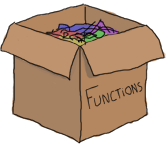
\includegraphics[width=1\linewidth]{modules.png}
\end{wrapfigure}

Работа с интерактивной оболочкой часто считается жизненно важной частью работы с динамическими языками программирования.
В ней удобно тестировать различный код и программы.
Чтобы использовать большую часть основных типов данных в Erlang, даже не нужно открывать текстовый редактор или сохранять файлы.
Можете отставить клавиатуру в сторону, сказать что на сегодня довольно, и пойти гулять.
Но если вы на этом остановитесь, то будете ужасным программистом на Erlang.
Чтобы использовать код, его нужно где\--то хранить!

Для этого и существуют модули.
Модуль \--- это несколько функций, сгруппированных в единый файл под одним именем.
Все функции в Erlang должны определяться в модулях.
Вы уже использовали модули, возможно даже не догадываясь об этом.
Встроенные функции \ops{hd} и \ops{tl}, которые упоминались в предыдущей главе, на самом деле входят в модуль \ops{erlang}, так же как и все арифметические, логические и булевы операторы.
ВФ из модуля \ops{erlang} отличаются от других функций тем, что при использовании Erlang они импортируются автоматически.
Вызов любой другой функции, определённой в модуле, должен выглядеть так: \ops{Module:Function(Arguments)}.

Смотрите:
\begin{lstlisting}[style=repl]
1> erlang:element(2, {a,b,c}).
b
2> element(2, {a,b,c}).
b
3> lists:seq(1,4).
[1,2,3,4]
4> seq(1,4).
** exception error: undefined shell command seq/2
\end{lstlisting}

В этом примере функция \ops{seq} из модуля list не была автоматически импортирована, тогда как \ops{element} была.
Ошибку ''undefined shell command'' генерирует оболочка, которая ищет и не находит команду оболочки (например, такую как \ops{f()}).
Некоторые функции из модуля \ops{erlang} не импортируются автоматически, но их используют не так часто.

Согласно логике, вы должны помещать функции, которые касаются похожих вещей, в один модуль.
Общие операции над списками хранятся в модуле \ops{lists}, а функции ввода\--вывода (которые позволяют выводить данные в консоль или файл), сгруппированы в модуле \ops{io}.
Единственный модуль, который не подчиняется этой схеме, это вышеупомянутый модуль \ops{erlang}, который содержит математические функции, функции преобразования, мультипроцессинга, изменения настроек виртуальной машины и т.д.
У этих функций нет ничего общего, кроме того, что все они считаются встроенными.
Лучше не создавать модули, похожие на \ops{erlang}, и сконцентрироваться на ясном логическом разделении функциональности.
\section{Объявление модуля}
\label{module-declaration}
\begin{wrapfigure}{l}{0.2\linewidth}
    
\includegraphics[width=1\linewidth]{declaration.png}
\end{wrapfigure}
Можно объявлять при написании модуля два вида сущностей: функции и атрибуты.
Атрибуты это метаданные, которые описывают сам модуль: его имя, функции, которые должны быть видимы снаружи, автора кода и прочее.
Эти метаданные весьма полезны, так как подсказывают компилятору, как он должен производить обработку, а также позволяют людям извлекать из скомпилированного кода полезную информацию, не обращаясь к исходному коду.

В Erlang существует большое количество разнообразных атрибутов модулей.
Вы и сами можете объявить любые атрибуты на собственный вкус.
Но также существуют некоторые предопределённые атрибуты, которые будут появляться в вашем коде чаще других.
Все атрибуты модулей записываются в форме \ops{-Name(Attribute).}.
Чтобы ваш модуль можно было скомпилировать, необходим лишь один атрибут:

\begin{minipage}{1\linewidth}
    \textbf{-module(Name).}\\ 
    Этот атрибут всегда указывается первым оператором в файле и обозначает имя текущего модуля, где \emph{Name} это ~\ref{atoms}~атом.
    Это имя используется при вызове функций из другого модуля.
    Вызовы записывают в виде \ops{M:F(A)}, где \emph{M} это имя модуля, \emph{F} это имя функции и \emph{A} её аргументы.
\end{minipage}

Настало время немного попрограммировать!
Наш первый модуль будет простым и бесполезным.
Откройте текстовый редактор, введите указанную ниже строку, и сохраните под именем \ops{useless.erl}:
\begin{lstlisting}[style=repl]
-module(useless).
\end{lstlisting}

Всего лишь одна эта строка уже является рабочим модулем.
Конечно, без функций в нём нет никакого смысла.
Сначала давайте решим, какие функции будут экспортироваться из нашего <<бесполезного>> модуля.
Для этого нам понадобится ещё один атрибут:

\begin{minipage}{1.0\linewidth}
    \textbf{-export([Function1/Arity, Function2/Arity,\ldots,FunctionN/Arity]).}\\ 
    Он используется для определения функций модуля, которые можно вызывать извне.
    Атрибут содержит список функций с соответствующей им арностью.
    Арность функции это целое число, которые соответствует количеству аргументов, которые принимает функция.
    Это важная информация, поскольку разные функции, определённые в модуле, могут иметь одинаковое имя, только если их арность различается.
    Поэтому функции \ops{add(X, Y)} и \ops{add(X, Y, Z)} будут считаться различными и записываться в виде \ops{add/2} и \ops{add/3} соответственно.
\end{minipage}

\colorbox{lgray}{
    \begin{minipage}{1\linewidth}
        \textbf{Замечание:} экспортируемые функции представляют собой интерфейс модуля.
        Важно чтобы интерфейс сообщал о модуле только то, что необходимо для его использования и ничего более.
        Это позволяет менять скрытые детали вашей реализации, не нарушая работу кода, который может полагаться на ваш модуль.
    \end{minipage}
}

Сначала наш модуль экспортирует полезную функцию под названием <<add>>, которая принимает два аргумента.
Атрибут \ops{-export} можно добавить после объявления модуля:
\begin{lstlisting}[style=repl]
-export([add/2]).
\end{lstlisting}

Теперь напишем функцию:
\begin{lstlisting}[style=erlang]
add(A,B) ->
    A + B.
\end{lstlisting}

Синтаксис функции соответствует виду \ops{Name(Args) $->$ Body.}, где \emph{Name} должен быть атомом, а \emph{Body} это одно, либо несколько выражений Erlang, разделённых запятыми.
Функция должна заканчиваться точкой.
Обратите внимание, что Erlang не использует ключевое слово <<return>>.
От <<return>> никакой пользы!
Вместо этого автоматически будет возвращён результат выполнения последнего выражения в функции, и вам ничего для этого не нужно будет делать.

Добавьте следующую функцию (конечно же, какое руководство без <<Hello world>>!
Хоть даже и в четвёртой главе!), и не забудьте добавить её в атрибут \ops{-export}.
\begin{lstlisting}[style=erlang]
%% Shows greetings.
%% io:format/1 is the standard function used to output text.
hello() ->
io:format("Hello, world!~n").
\end{lstlisting}

Из этой функции нам станет понятно, что каждый комментарий должен начинаться с символа \ops{\%} и состоять из одной строки (то, что в примере используется \ops{\%\%}, не более чем вопрос стиля).
Также функция \ops{hello/0} демонстрирует как в вашем модуле можно вызывать функции из внешних модулей.
В данном случае это функция \ops{io:format/1}, которая является стандартной функцией для вывода текста (что объясняется в комментарии).

Добавим ещё одну функцию, которая будет использовать и \ops{add/2}, и \ops{hello/0}:
\begin{lstlisting}[style=erlang]
greet_and_add_two(X) ->
    hello(),
    add(X,2).
\end{lstlisting}
\begin{wrapfigure}[8]{l}{0.3\linewidth}
    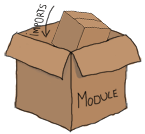
\includegraphics[width=1\linewidth]{imports.png}
\end{wrapfigure}

Не забудьте добавить\ops{greet\_and\_add\_two/1} в список экспортируемых функций.
Для вызовов \ops{hello/0} и \ops{add/2} указывать имя модуля не нужно, так как они были объявлены в текущем модуле.

Если бы вы захотели вызвать функцию \ops{io:format/1} так же как \ops{add/2} или любую другую функцию, определённую внутри модуля, то вам нужно было бы добавить в начале файла следующий атрибут: \ops{-import(io, [format/1]).}.
После этого можно сделать вызов \ops{format(''Hello, World!\~\strut n'').} напрямую.
Общий вид атрибута \ops{-import} подчиняется следующей формуле:
\begin{lstlisting}[style=erlang]
-import(Module, [Function1/Arity,..., FunctionN/Arity]).
\end{lstlisting}

Импорт функции это просто быстрый способ получить к ней доступ.
Программистам на Erlang не рекомендуется использовать атрибут \ops{-import}, так как считается, что это уменьшает читаемость кода.
К примеру, помимо функции \ops{io:format/2} существует также и функция \ops{io\_lib:format/2}.
Чтобы понять, какую из них использовал программист, придётся перейти в начало файла и посмотреть, из какого модуля функция была импортирована.
Поэтому использование имени модуля в качестве префикса считается хорошим стилем.
Обычно импортируют лишь функции, определённые в модуле lists, так как они используются намного чаще других.

Теперь ваш модуль \ops{useless} должен принять следующий вид:
\begin{lstlisting}[style=erlang]
-module(useless).
-export([add/2, hello/0, greet_and_add_two/1]).
 
add(A,B) ->
A + B.
 
%% Shows greetings.
%% io:format/1 is the standard function used to output text.
hello() ->
io:format("Hello, world!~n").
 
greet_and_add_two(X) ->
hello(),
add(X,2).
\end{lstlisting}

Мы закончили работать с нашим модулем <<useless>>.
Можете сохранить файл под именем \ops{useless.erl}.
Имя файла должно состоять из имени модуля, определённого в атрибуте \ops{-module}, и заканчиваться расширением '.erl', которое стандартно используется для файлов с исходным кодом Erlang.

Перед тем как скомпилировать модуль и, наконец\--то, опробовать его в деле, мы увидим как определять и использовать макросы.
В Erlang макросы очень похожи на выражения <<\#define>> в языке C, и, главным образом, используются для определения коротких функций и констант.
Они представляют собой простые текстовые выражения, которые будут заменены перед компиляцией кода.
Макросы полезны для того, чтобы не раскидывать по тексту ваших модулей <<магические>> значения.
Макрос определяется как атрибут модуля в виде \ops{-define(MACRO, some\_value).} и его можно использовать внутри модуля как \ops{?MACRO}.
Макрос в виде <<функции>> можно записать как \ops{-define(sub(X, Y), X - Y).} и использовать в виде \ops{?sub(23, 47)}.
Такой макрос позже будет заменён компилятором на выражение \ops{23 - 47}.
Кто\--то использует более сложные макросы, но общий синтаксис не меняется.
\section{Компилируем код}
\label{compiling-the-code}
Чтобы код Erlang мог использоваться виртуальной машиной, его компилируют в байт\--код.
Компилятор можно вызывать несколькими способами: из командной строки как \ops{\$ erlc flags file.erl}, из оболочки или в модуле как \ops{compile:file(FileName)}, в оболочке как \ops{c()} и т.д.

Пора скомпилировать наш бесполезный модуль и опробовать его.
Откройте оболочку Erlang и введите:
\begin{lstlisting}[style=erlang]
1> cd("/path/to/where/you/saved/the-module/").
"Path Name to the directory you are in"
ok
\end{lstlisting}

Оболочка будет искать по умолчанию файлы в той же директории, из которой она стартовала, а также в стандартной библиотеке.
Функция \ops{cd/1} определена только в оболочке Erlang.
Она позволяет изменить текущую директорию.
Пользователи Windows должны использовать в качестве разделителя директорий прямой слеш (косую черту \ops{\//}).
Когда мы поменяли текущую директорию на ту, в которой содержится наш модуль, вводим следующую команду:
\begin{lstlisting}[style=erlang]
2> c(useless).
{ok,useless}
\end{lstlisting}

Если сообщение, которое вы получили, отличается от приведённого выше, то убедитесь что файл назван правильно, что вы находитесь в правильной директории и в вашем модуле нет ошибок.
Когда компиляция пройдёт успешно, вы увидите, что в директории помимо \ops{useless.erl} появился ещё один файл \--- \ops{useless.beam}.
Это скомпилированный модуль.
Попробуем воспользоваться нашими функциями:
\begin{lstlisting}[style=erlang]
3> useless:add(7,2).
9
4> useless:hello().
Hello, world!
ok
5> useless:greet_and_add_two(-3).
Hello, world!
-1
6> useless:not_a_real_function().
** exception error: undefined function useless:not_a_real_function/0
\end{lstlisting}

Функции работают как и было задумано: \ops{add/2} складывает числа, \ops{hello/0} выводит <<Hello, world!>>, а \ops{greet\_and\_add\_two/1} делает и то и другое!
Вы, вероятно, задали себе вопрос: а почему функция \ops{hello/0} после вывода текста возвращает атом <<ok>>?
Потому что функции и выражения в Erlang \textbf{всегда} должны что\--то возвращать, даже когда в других языках они это делать не обязаны.
Поэтому функция \ops{io:format/1} возвращает <<ok>>, чтобы обозначить, что выполнение прошло нормально и ошибки отсутствуют.

В выражении 6 отображена ошибка, которая была сгенерирована из\--за отсутствия функции.
Если вы забыли проэкспортировать функцию, то получите сообщение именно такого типа.\\ 
\colorbox{lgray}
{
    \begin{minipage}{1\linewidth}
        \textbf{Замечание:} расширение '.beam', если вам интересно, означает \emph{Bogdan/Björn's Erlang Abstract Machine} (так называется виртуальная машина).
        Существуют также и другие виртуальные машины для Erlang, но сейчас они не более чем достояние истории, и их не используют.
        Среди них JAM (Joe's Abstract Machine, вобравшая черты Prolog WAM, и старая BEAM, которая предпринимала попытки компиляции из Erlang в C, и после \--- в нативный код.
        Измерения показали, что выигрыш от применения этого метода был слишком мал, поэтому от него отказались.
    \end{minipage}
}

Существует много флагов, которые позволяют тоньше контролировать процесс компиляции модуля.
Их список можно найти в \href{http://erlang.org/doc/man/compile.html}{документации Erlang}.
Вот наиболее востребованные флаги:\\ 

\begin{minipage}{0.9\linewidth}
    \textbf{-debug\_info}\\ 
    Добавляет в модуль отладочную информацию, которая необходима для работы инструментов Erlang, таких как отладчик, утилиты статического анализа и покрытия кода.
\end{minipage}

\begin{minipage}{0.9\linewidth}
    \textbf{-\{outdir,Dir\}}\\ 
    Компилятор Erlang будет по умолчанию создавать ''beam'' файлы в текущей директории.
    Этот флаг позволяет задать путь к директории, в которой будут сохраняться скомпилированные файлы.
\end{minipage}

\begin{minipage}{0.9\linewidth}
    \textbf{-export\_all}\\ 
    Флаг заставляет игнорировать атрибут модуля \ops{-export}.
    При этом будут проэкспортированы все функции, которые в нём определены.
    Главным образом этот флаг полезен при тестировании и разработке нового кода, и его не следует использовать на рабочих системах.
\end{minipage}

\begin{minipage}{0.9\linewidth}
    \textbf{\{d,Macro\} или \{d,Macro,Value\}}\\ 
    Определяет макрос, который можно будет использовать в модуле.
    \emph{Macro} должен быть атомом.
    Чаще всего этот флаг используется при юнит\--тестировании, чтобы гарантировать, что тестовые функции будут создаваться и экспортироваться только когда в них есть необходимость.
    По умолчанию элемент \emph{Value} имеет значение <<true>>, если не указан в списке явно.
\end{minipage}

Чтобы скомпилировать наш модуль \ops{useless} с использованием флагов, нужно выполнить одну из следующих директив:
\begin{lstlisting}[style=erlang]
7> compile:file(useless, [debug_info, export_all]).
{ok,useless}
8> c(useless, [debug_info, export_all]).
{ok,useless}
\end{lstlisting}

Также можно схитрить и определить флаги компиляции при помощи атрибутов прямо в самом модуле.
Чтобы получить такой же результат как в выражениях 7 и 8, необходимо добавить в модуль следующую строку: 
\begin{lstlisting}[style=erlang]
-compile([debug_info, export_all]).
\end{lstlisting}

Далее необходимо лишь скомпилировать модуль, и вы получите тот же результат, что и с флагами переданными вручную.
А теперь, когда мы можем записывать функции, компилировать их и исполнять, настало время узнать, что же мы сможем со всем этим сделать!\\ 
\colorbox{lgray}
{
    \begin{minipage}{1\linewidth}
        \textbf{Замечание:} модуль также можно скомпилировать в нативный код.
        Компиляция в нативный код доступна не для каждой платформы и ОС.
        Для платформ, которые допускают такую компиляцию, можно добиться ускорения программ (по неточным данным приблизительно на 20\%).
        Для компиляции в нативный код необходимо использовать модуль \ops{hipe}. Компиляция осуществляется при помощи команды: \ops{hipe:c(Module,OptionsList).}
        Также в оболочке можно использовать команду \ops{c(Module,[\{hipe,o3\}]).}
        Обратите внимание, что .beam файл, полученный в результате такой компиляции, нельзя переносить между платформами, тогда как обычные файлы можно.
    \end{minipage}
}
\section{Подробнее о модулях}
\label{more-about-modules}
Прежде чем переходить к написанию функций и кода, польза которых сомнительна, необходимо упомянуть ещё несколько фактов, которые в будущем могут пригодиться.

Первый из них касается метаданных в модулях.
Я упомянул в начале главы, что атрибуты модуля \---это метаданные, которые описывают сам модуль.
Как мы можем получить доступ к этим метаданным, если у нас нет доступа к исходному коду модуля?
В этом нам поможет компилятор.
При компиляции он соберёт атрибуты и сохранит их (вместе с другой информацией) в функции \ops{module\_info/0}.
Вот так будут выглядеть метаданные модуля \ops{useless}:
\begin{lstlisting}[style=erlang]
9> useless:module_info().
[{exports,[{add,2},
            {hello,0},
            {greet_and_add_two,1},
            {module_info,0},
    {module_info,1}]},
    {imports,[]},
    {attributes,[{vsn,[174839656007867314473085021121413256129]}]},
    {compile,[{options,[]},
            {version,"4.6.2"},
            {time,{2009,9,9,22,15,50}},
{source,"/home/ferd/learn-you-some-erlang/useless.erl"}]}]
10> useless:module_info(attributes).
[{vsn,[174839656007867314473085021121413256129]}]
\end{lstlisting}

Также в вышеприведённом тексте есть упоминание дополнительной функции \ops{module\_info/1}, которая позволит получить каждый элемент метаданных по отдельности.
В метаданных содержатся экспортируемые функции, импортируемые функции (в данном случае ни одной), атрибуты (в них можно хранить метаданные, которые определены вами), информация о компиляции и ключи компиляции.
Если бы вы решили добавить в модуль атрибут \ops{-author(``An Erlang Champ'').}, он оказался бы в том же разделе, где и \ops{vsn}.
Когда дело доходит до рабочей системы, для атрибутов модулей маловато применений, но они могут быть полезны для реализации маленьких хитростей: я использую их в \href{http://learnyousomeerlang.com/static/erlang/tester.erl}{тестовом скрипте}, чтобы описывать функции, для которых юнит\--тесты оставляют желать лучшего.
Скрипт сканирует атрибуты модуля, находит функции, снабжённые комментариями, и выдаёт о них предупреждения.\\ 
\colorbox{lgray}
{
    \begin{minipage}{1\linewidth}
        \textbf{Замечание:} \ops{vsn} это уникальное значение, которое генерируется автоматически и отличается для каждой версии вашего кода, исключая комментарии.
        Это значение используется при горячей загрузке кода (обновление приложения во время исполнения, без необходимости его остановки), а также некоторыми инструментами, которые связаны с управлением релизами.
        Если хотите, можете сами указать значение для \ops{vsn}: просто добавьте в модуль атрибут \ops{-vsn(VersionNumber)}.
    \end{minipage}
}

\begin{wrapfigure}{r}{0.4\linewidth}
    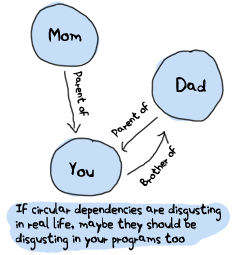
\includegraphics[width=1\linewidth]{circular-dependencies.png}
\end{wrapfigure}
Ещё один момент, на который стоит обратить внимание при проектировании модулей: избегайте циклических зависимостей!
Модуль \emph{A} не должен вызывать модуль \emph{B}, который в свою очередь вызывает модуль \emph{A}.
Такие зависимости приводят к усложнению поддержки кода.
Кому хочется проснуться посреди ночи от того, что маньяк\--разработчик пытается выдавить вам глаза из\--за чудовищного кода, который вы написали.

По той же причине (поддержка кода и забота о вашим зрении), обычно считается хорошим тоном размещение рядом функций близких по назначению.
В качестве примера можно привести функции запуска и остановки приложения, или создания и удаления записи в некоторой базе данных.

Ну что ж, довольно нравоучений.
Готовы узнать ещё немного об Erlang?

\chapter{Синтаксис функций}
\label{syntax-in-functions}
\section{Сопоставление с образцом}
\begin{wrapfigure}{r}{0.3\linewidth}
    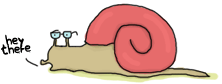
\includegraphics[width=1\linewidth]{snail.png}
\end{wrapfigure}
Теперь, когда у нас есть возможность сохранять и компилировать наш код, мы можем начать писать более сложные функции. Те, что мы написали раньше, были чрезвычайно просты и восторгаться в них было нечем. Перейдём к более интересным вещам. Первая функция, которую мы напишем, будет выдавать различные приветствия в зависимости от переданного ей пола. В большинстве языков нужно было бы написать что\--то близкое к этому:
\begin{lstlisting}[style=erlang]
function greet(Gender,Name)
    if Gender == male then
        print("Hello, Mr. %s!", Name)
    else if Gender == female then
        print("Hello, Mrs. %s!", Name)
    else
        print("Hello, %s!", Name)
end
\end{lstlisting}

С использованием сопоставления с образцом, Erlang позволяет избавиться от кучи шаблонного кода. В Erlang подобная функция будет выглядеть так:
\begin{lstlisting}[style=erlang]
greet(male, Name) ->
    io:format("Hello, Mr. ~s!", [Name]);
greet(female, Name) ->
    io:format("Hello, Mrs. ~s!", [Name]);
greet(_, Name) ->
    io:format("Hello, ~s!", [Name]).
\end{lstlisting}

Признаю, что функция вывода в Erlang выглядит намного уродливее, чем в других языках, но смысл не в этом. Главное отличие в том, что при использовании сопоставления с образцом, мы убили сразу двух зайцев: определили, какие части функции будут использованы, и связали значения с переменными. Нам не нужно сначала связывать значения, а потом их сравнивать! Поэтому вместо:
\begin{lstlisting}[style=erlang]
function(Args)
    if X then
        Expression
    else if Y then
        Expression
    else
        Expression
\end{lstlisting}
Мы напишем:
\begin{lstlisting}[style=erlang]
function(X) ->
    Expression;
function(Y) ->
    Expression;
function(_) ->
    Expression.
\end{lstlisting}

и придём к тем же результатам, используя более декларативный стиль. Каждое объявление \ops{function} называется \emph{функциональным выражением}. Функциональные выражения должны разделяться символом точки с запятой (\ops{;}) и вместе они формируют \emph{объявление функции}. Объявление функции считается одной большой конструкцией, поэтому заключительное функциональное выражение завершается точкой. Этот способ использования элементов для определения потока задач (workflow), может показаться немного <<странным>>, но вы к нему привыкнете. Ну или хотя бы надейтесь на то, что это случится, потому что иного пути не существует!\\
\colorbox{lgray}
{
    \begin{minipage}{1\linewidth}
        \textbf{Замечание:} форматирование при помощи \ops{io:format} осуществляется при помощи токенов, которые определяют замены в строке. Для обозначения токенов используется символ тильды (\ops{\strut\mytilde}). Есть встроенные токены, например\ops{\mytilde n}. Этот токен будет преобразован в перевод строки. Большинство других токенов обозначают способ форматирования данных. Например, вызов функции \ops{io:format(``\mytilde s!\mytilde n'',[``Hello'']).} заключает в себе токен \ops{\mytilde n}, и токен \ops{\mytilde s}, который в качестве аргументов принимает строки и битовые строки. После применения форматирования, строка примет вид \ops{``Hello!\\n''}. Ещё одним широко используемым токеном является \ops{\mytilde p}. Он печатает содержимое переменной Erlang, учитывая форматирование (с добавлением отступов и всего прочего).\\ 
        Мы ознакомимся с подробностями применения функции \ops{io:format} в последующих главах, когда будем углублённо работать с вводом/выводом. Но сейчас можете попробовать исполнить следующие вызовы функций: \ops{io:format(''\mytilde s\mytilde n'',[$<<$''Hello''$>>$])}, \ops{io:format''\mytilde p\mytilde n'', [$<<$''Hello''$>>$])}, \ops{io:format(''\mytilde\mytilde\mytilde n'')}, \ops{io:format(''\mytilde f\mytilde n'', [4.0])}, \ops{io:format(''\mytilde 30f\mytilde n'', [4.0])}. Это лишь малая часть возможных операций. Команды немного похожи на \ops{printf} из другого языка. Если не можете дотерпеть до главы, в которой описывается ввод/вывод, то почитайте \href{http://erlang.org/doc/man/io.html\#format-3}{документацию онлайн}.
    \end{minipage}
}

В функциях сопоставление с образцом может принимать ещё более сложные и мощные формы. Как вы, может быть, помните, несколько глав назад мы применяли сопоставление с образцом, чтобы получать головную и хвостовую части списков. Давайте попробуем это сделать снова! Создайте новый модуль и назовите его \ops{functions}. В нём мы напишем несколько функций, которые позволят нам исследовать пути использования сопоставления с образцом:
\begin{lstlisting}[style=erlang]
-module(functions).
-compile(export_all). %% replace with -export() later, for God's sake!
\end{lstlisting}

Первой нашей функцией станет \ops{head/1}, которая будет вести себя точно так же как \ops{erlang:hd/1}: принимать список в качестве аргумента и возвращать его первый элемент. Мы будем это делать при помощи оператора cons (\ops{\strut|}):
\begin{lstlisting}[style=erlang]
head([H|_]) -> H.
\end{lstlisting}

Если вы введёте в оболочке \ops{functions:head([1,2,3,4]).} (после того как скомпилируете модуль), то вам будет возвращено значение '1'. Чтобы получить второй элемент, следовательно, вам нужно создать функцию: 
\begin{lstlisting}[style=erlang]
second([_,X|_]) -> X.
\end{lstlisting}

Список будет разобран Erlang при помощи сопоставления с образцом. Поробуйте выполнить эту операцию в оболочке!
\begin{lstlisting}[style=erlang]
1> c(functions).
{ok, functions}
2> functions:head([1,2,3,4]).
1
3> functions:second([1,2,3,4]).
2
\end{lstlisting}

Можно повторять этот процесс для списков сколько угодно, но для тысячи значений это было бы непрактично. Для того чтобы это исправить, мы будем писать рекурсивные функции, которые разберём чуть позже. А сейчас давайте сосредоточимся на сопоставлении с образцом. Концепция свободной и связанной переменной, которую мы обсуждали в главе ~\ref{starting-out-for-real}~также справедлива и для функций. Мы можем сравнивать и выяснять, одинаковы ли два параметра, которые переданы в функцию. Для этого мы создадим функцию \ops{same/2}, которая принимает два аргумента и сообщает, совпадают ли они друг с другом:
\begin{lstlisting}[style=erlang]
same(X,X) ->
true;
same(_,_) ->
false.
\end{lstlisting}

Вот так всё просто. Прежде чем объяснять как работают функции, мы ещё раз повторим концепцию связанной и свободной переменной, на всякий случай:
\begin{wrapfigure}{i}{0.7\linewidth}
    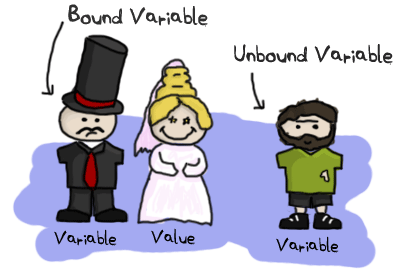
\includegraphics[width=1\linewidth]{un-bound.png}
\end{wrapfigure}
На этой картинке жених опечален, потому что в Erlang переменные никогда не могут менять значение: конец свободе! А если серьёзно, то свободными называются переменые, у которых ничего нет (как у нашего маленького бомжика справа). Процесс связывания переменной заключается в простом присоединении значения к свободной переменной. Если вы захотите присвоить значение связанной переменной, Erlang сгенерирует ошибку. Но ошибки не будет, если новое значение совпадает со старым. Представим, что парень слева женится на девушке, у которой есть сестра\--близнец. Если рядом появится сестра, жених не отличит её от невесты, и никак не отреагирует. Если же появится посторонняя женщина, жених будет недоволен. Если вам неясна эта концепция, можете вернуться к разделу о \ref{invariable-variables}~Неизменных переменных.

Вернёмся к нашему коду. Когда вы вызовете функцию \ops{same(a,a)}, то первая переменная \emph{X} считается свободной и автоматически принимает значение \ops{a}. Далее Erlang переходит ко второму аргументу, видит что переменная \emph{X} уже связана. После этого он сравнивает её со значением \ops{a}, которое было передано в качестве второго аргумента, и определяет, совпадают ли они друг с другом. Операция сопоставления с образцом завершается успешно и функция возвращает \ops{true}. Если два значения различаются, то сравнение завершится неудачей, и управление перейдёт к второму функциональному выражению, которое не проверяет аргументы (когда выбирать не из чего, нечего перебирать!), а просто возвращает false. Заметьте, что эта функция может фактически принимать абсолютно любые аргументы! Она работает не только со списками или с одиночными переменными, а с любыми типами данных. Рассмотрим пример посложнее: функцию, которая печатает дату, но лишь тогда, когда она правильно отформатирована:
\begin{lstlisting}[style=erlang]
valid_time({Date = {Y,M,D}, Time = {H,Min,S}}) ->
    io:format("The Date tuple (~p) says today is: ~p/~p/~p,~n",[Date,Y,M,D]),
    io:format("The time tuple (~p) indicates: ~p:~p:~p.~n", [Time,H,Min,S]);
valid_time(_) ->
    io:format("Stop feeding me wrong data!~n").
\end{lstlisting}

Есть также возможность использовать оператор \ops{\strut=}, который позволяет сопоставлять не только содержимое кортежа (\ops{\{Y,M,D\}}), но и сам кортеж в целом (\emph{Date}). Функцию можно протестировать следующим образом:
\begin{lstlisting}[style=erlang]
4> c(functions).
{ok, functions}
5> functions:valid_time({{2011,09,06},{09,04,43}}).
The Date tuple ({2011,9,6}) says today is: 2011/9/6,
The time tuple ({9,4,43}) indicates: 9:4:43.
ok
6> functions:valid_time({{2011,09,06},{09,04}}).
Stop feeding me wrong data!
ok
\end{lstlisting}

Правда есть одна проблема! Эта функция будет принимать в качестве входящих данных что угодно, даже текст или атомы. Достаточно лишь, чтобы кортежи имели вид \ops{\{\{A,B,C\}, \{D,E,F\}\}}. Вот мы и пришли к одному из ограничений сопоставления с образцом: с его помощью можно указать либо очень точные значения, например известное число или атом, либо абстрактные значения, такие как голова|хвост списка, кортеж из \emph{N} элементов, или что угодно другое (\ops{\strut\_} и свободные переменные), и т.д. Чтобы решить эту проблему мы используем охранные выражения, стражи (guards). 
\section{Стража! Стража!}
    Стражи \--- это дополнительные выражения, которые можно добавлять в заголовки функций, чтобы сделать сопоставление с образцом более выразительным. Как уже упоминалось выше, в сопоставлении с образцом есть ограничения, так как с его помощью нельзя сопоставлять, к примеру, диапазон значений, или  определённые типы данных. Мы не можем выразить концепцию счёта: слишком ли низок этот двенадцатилетний баскетболист, чтобы играть с профессионалами? Слишком ли велика эта дистанция, чтобы пройти её на руках? Ты слишком стар, или слишком молод, чтобы водить машину? На такие вопросы не ответишь, применяя лишь простое сопоставление с образцом. Конечно, можно представить вопрос про вождение в таком виде:
\begin{lstlisting}[style=erlang]
old_enough(0) -> false;
old_enough(1) -> false;
old_enough(2) -> false;
...
old_enough(14) -> false;
old_enough(15) -> false;
old_enough(_) -> true.
\end{lstlisting}

Но это уж слишком громоздко. Если хотите, можете так делать, но будьте готовы работать над своим кодом в гордом одиночестве. Если всё же хотите со временем обзавестись друзьями, создайте новый модуль \ops{guards}, в котором мы реализуем <<правильное>> решение для вопроса о вождении:
\begin{lstlisting}[style=erlang]
old_enough(X) when X >= 16 -> true;
old_enough(_) -> false.
\end{lstlisting}

Вот и всё! Как видите, такая запись намного короче и понятнее. Основное правило для охранных выражений: чтобы выражение сработало, оно должно возвращать \ops{true}. Если страж возвращает \ops{false}, или бросает исключение, то оно не срабатывает. Предположим, что мы хотим запретить садиться за руль людям старше 104 лет. Водить можно только в возрасте от 16 до 104 лет. Как же нам выполнить это условие? Давайте просто добавим второе охранное выражение:
\begin{lstlisting}[style=erlang]
right_age(X) when X >= 16, X =< 104 ->
    true;
right_age(_) ->
    false.
\end{lstlisting}

Запятая (\ops{\strut,}) по выполняемой роли похожа на оператор\ops{andalso}, а точка с запятой (\ops{;}) ведёт себя приблизительно как\ops{orelse} (эти операторы описаны в разделе \ref{boolandcompare}~Булева алгебра и операторы сравнения). Чтобы всё выражение успешно выполнилось, необходимо чтобы было удовлетворено условие в обоих охранных выражениях. Также можно поменять условия в функции на противоположные:
\begin{lstlisting}[style=erlang]
wrong_age(X) when X < 16; X > 104 ->
    true;
wrong_age(_) ->
    false.
\end{lstlisting}
\begin{wrapfigure}{l}{0.2\linewidth}
    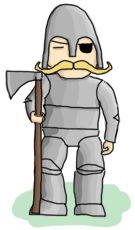
\includegraphics[width=1\linewidth]{guard.png}
\end{wrapfigure}

И с этим выражением мы всё равно получим правильные результаты. Если хотите, можете протестировать (вы всегда должны всё проверять!). В охранных выражениях точка с запятой (\ops{;}) ведёт себя как оператор\ops{orelse}: если первый страж не исполняется, то исполнение переходит ко второму, потом к следующему, до тех пор пока хотя бы один страж возвратит истину или все стражи возвратят ложь.

Помимо функций сравнения и булевых операторов, можно использовать и другие функции, включая математические операции (\ops{A*B\//C >= 0}) и функции определения типа, такие как \ops{is\_integer/1}, \ops{is\_atom/1}, и т.д. (Мы вернёмся к ним в следующей главе). Одним из недостатков охранных выражений является то, что они не принимают функции определённые пользователем из\--за возможных побочных эффектов. Erlang не чистый функциональный язык программирования (коим является, к примеру, \href{http://learnyouahaskell.com}{Haskell}) потому что во многом полагается на побочные эффекты: можно выполнять операции ввода\--вывода, пересылать между акторами сообщения, выбрасывать исключения когда угодно и где угодно. Не существует простого способа определить, что функция, которая используется в охранном выражении, печатает текст. А может быть не печатает. А может быть она перехватывает важные сообщения об ошибках при тестировании в нескольких функциональных выражениях. Поэтому Erlang просто вам не доверяет (и, скорее всего, правильно делает!)

    После всего сказанного, у вас должно было появиться понимание базового синтаксиса охранных выражений, достаточное для того чтобы не теряться при встрече с ними.\\
\colorbox{lgray}
{
    \begin{minipage}{\linewidth}
        \textbf{Замечание:} я сравнивал символы \ops{,} и \ops{;} в охранных выражениях с операторами \ops{andalso} и \ops{orelse}. По правде говоря, они не совсем эквивалентны. Первые будут захватывать возникающие исключения, а вторые не будут. Это означает, что если в первой части охранного выражения \ops{X $>=$ N; N $>=$ 0} будет сгенерирована ошибка, то вторая часть всё же будет исполнена, и выражение может сработать. Если ошибка была выброшена в первой части выражения \ops{X $>=$ N orelse N $>=$ 0}, то вторая часть будет пропущена, и всё охранное выражение не сработает.\\ 
        Однако (всегда есть какое\--нибудь <<однако>>) только операторы \ops{andalso} и \ops{orelse} могут помещаться в охранное выражение. Это означает, что \ops{(A orelse B) andalso C} это валидное выражение, а \ops{(A; B), C} \--- нет. Нужно учитывать их различное назначение и использовать в сочетании друг с другом.
    \end{minipage}
}

\section{Что ещё за <<If>>?!}
\ops{If}\--ы ведут себя подобно охранным выражениям и имеют тот же синтаксис, но используются за пределами заголовка функции. Они даже называются \emph{Охранными шаблонами}. \ops{if}\--ы в Erlang отличаются от \ops{if}\--ов в большинстве других языков. По сравнению с ними, это странные создания, которых принимали бы охотнее, называйся они иначе. Вступая в страну Erlang, оставьте всё что вы знаете об \ops{if} на пороге. Займите своё место \--- мы отправляемся в путешествие.

Чтобы понять как похожи выражения \ops{if} на охранные выражения, взгляните на следующие примеры:
\begin{lstlisting}[style=erlang]
-module(what_the_if).
-export([heh_fine/0]).
 
heh_fine() ->
    if 1 =:= 1 ->
        works
    end,
    if 1 =:= 2; 1 =:= 1 ->
        works
    end,
    if 1 =:= 2, 1 =:= 1 ->
        fails
    end.
\end{lstlisting}
Сохраним этот код в файл \ops{what\_the\_if.erl}, и попробуем его исполнить:
\begin{lstlisting}[style=repl]
1> c(what_the_if).
./what_the_if.erl:12: Warning: no clause will ever match
./what_the_if.erl:12: Warning: the guard for this clause evaluates to 'false'
{ok,what_the_if}
2> what_the_if:heh_fine().
** exception error: no true branch found when evaluating an if expression
    in function  what_the_if:heh_fine/0
\end{lstlisting}
Ой! Компилятор нас предупреждает, что условие if в строке 12 (\ops{1 =:= 2, 1 =:= 1}) никогда не будет использовано, так как его единственное охранное выражение всегда возвращает \ops{false}. Помните, в Erlang всё должно что\--то возвращать, и \ops{if}\-- выражения не являются исключением из этого правила. 
\begin{figure}[h!]
    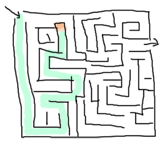
\includegraphics[width=0.3\linewidth]{labyrinth.png}
\end{figure}
Таким образом, когда Erlang не может найти случай, в котором страж успешно выполнится, будет сгенерирована ошибка: возвращать в этом случае нечего. Поэтому мы должны добавить ветвь, которая будет успешно исполняться не смотря ни на что. В большинстве языков это бы называлось 'else'. В Erlang мы используем слово 'true' (это объясняет, почему VM сгенерировала сообщение <<no true branch found>>)
\begin{lstlisting}[style=erlang]
oh_god(N) ->
    if N =:= 2 -> might_succeed;
        true -> always_does  %% this is Erlang's if's 'else!'
    end.
\end{lstlisting}

Если мы теперь протестируем эту новую функцию (старая будет продолжать плеваться предупреждениями. Можно их игнорировать или оставить как напоминание о том, как делать нельзя):
\begin{lstlisting}[style=erlang]
3> c(what_the_if).
./what_the_if.erl:12: Warning: no clause will ever match
./what_the_if.erl:12: Warning: the guard for this clause evaluates to 'false'
{ok,what_the_if}
4> what_the_if:oh_god(2).
might_succeed
5> what_the_if:oh_god(3).
always_does
\end{lstlisting}

Вот ещё одна функция, которая показывает как использовать несколько стражей в \ops{if}\--выражении. Эта же функция также демонстрирует, что любое выражение должно что\--нибудь возвращать: к переменной \emph{Talk} привязывается результат выражения \ops{if} и затем конкатенируется в строку, которая входит в состав кортежа. Читая код, легко увидеть как отсутствие ветки \ops{true} могло бы всё испортить, если учитывать, что в Erlang не существует такого понятия как null\--значение (как nil в lisp, NULL в C, None в Python и т.д.):
\begin{lstlisting}[style=erlang]
%% note, this one would be better as a pattern match in function heads!
%% I'm doing it this way for the sake of the example.
help_me(Animal) ->
    Talk = if Animal == cat  -> "meow";
            Animal == beef -> "mooo";
            Animal == dog  -> "bark";
            Animal == tree -> "bark";
            true -> "fgdadfgna"
        end,
    {Animal, "says " ++ Talk ++ "!"}.
\end{lstlisting}
А теперь попробуем исполнить:
\begin{lstlisting}[style=erlang]
6> c(what_the_if).
./what_the_if.erl:12: Warning: no clause will ever match
./what_the_if.erl:12: Warning: the guard for this clause evaluates to 'false'
{ok,what_the_if}
7> what_the_if:help_me(dog).
{dog,"says bark!"}
8> what_the_if:help_me("it hurts!").
{"it hurts!","says fgdadfgna!"}
\end{lstlisting}
Как и множество программистов на Erlang, вы, должно быть, недоумеваете \--- почему 'true' взяло верх над 'else' в качестве атома для управления потоком исполнения? В конце концов, 'else' более привычен. Richard O'Keefe дал в почтовой рассылке Erlang следующий ответ на этот вопрос. Я привожу его здесь без купюр, потому что сам не смог бы сформулировать лучше:\\
\colorbox{lgray}
{
    \begin{minipage}{\linewidth}
    Может быть 'else' и привычнее, но это не означает, что 'else' это хорошо. Я понимаю, что при помощи выражения '; true ->' очень легко получить в Erlang 'else', но результаты двух десятков лет наблюдений за психологией программирования показывают, что ни к чему хорошему это не приведёт. Я начал заменять:
\end{minipage}
}
\begin{lstlisting}[style=erlang]
if X > Y -> a()
    ; true  -> b()
if X > Y -> a()
    ; X < Y -> b()
    ; true  -> c()
end
\end{lstlisting}
\colorbox{lgray}
{
    \begin{minipage}{\linewidth}
на
    \end{minipage}
}
\begin{lstlisting}[style=erlang]     
if X > Y  -> a()
    ; X =< Y -> b()
end

if X > Y -> a()
    ; X < Y -> b()
    ; X == Y -> C()
end
\end{lstlisting}
\colorbox{lgray}
{
    \begin{minipage}{\linewidth}
это немного раздражает, когда я \textbf{пишу} код, но чрезвычайно помогает, когда я его \textbf{читаю}.
    \end{minipage}
}

Лучше всего <<избегать>> и 'else' и 'true': \ops{if}\--ы обычно легче читать, когда явно покрываются все логические исходы, без использования выражения, которое <<ловит всё подряд>>.

Как упоминалось ранее, в охранных выражениях можно использовать ограниченный набор функций (мы ещё с ними встретимся в \ref{types-or-lack-thereof}~Типы (или их отсутствие). Настало время явить подлинную мощь условных операторов Erlang. Я представляю вам выражение \ops{case}!\\
\colorbox{lgray}
{
    \begin{minipage}{\linewidth}
\textbf{Замечание:} весь ужас, отражённый в названиях функций файла \ops{what\_the\_if.erl}, относится к языковой конструкции \ops{if}, если рассматривать её с точки зрения \ops{if} любого другого языка. В контексте Erlang эта конструкция оказывается абсолютно логичной, просто её имя сбивает с толку.
    \end{minipage}
}
\section{В случае\ldots если}

Если считать, что выражения \ops{if} похожи на стражей, то \ops{case \ldots of} похоже на заголовок функции в целом. Для каждого аргумента можно применять сложные выражения сопоставления с образцом и, вдобавок, использовать стражи!

Так как вы уже неплохо знакомы с синтаксисом, нам не понадобится много примеров. На этот раз мы напишем функцию дополнения (append) для множеств (sets) (набор уникальных значений), который мы представим как неупорядоченный список. В смысле эффективности это, пожалуй, наихудшая возможная реализация наборов, но сейчас мы заботимся не об эффективности, а о синтаксисе:
\begin{lstlisting}[style=erlang]
insert(X,[]) ->
    [X];
insert(X,Set) ->
    case lists:member(X,Set) of
        true  -> Set;
        false -> [X|Set]
    end.
\end{lstlisting}
Если мы передаём в функцию пустое множество (список) и терм \emph{X}, она возвращает нам список, который содержит лишь \emph{X}. Иначе, функция \ops{lists:member/2} проверяет, не является ли элемент частью списка, и возвращает true, если является и false, если нет. В случае, когда в нашем множестве уже присутствует элемент \emph{X}, нам не нужно изменять список. Если элемента в списке нет, то мы добавляем \emph{X} первым элементом списка.

В нашем примере, сопоставление с образцом было очень простым. Оно может усложняться (можете сравнить ваш код с \href{http://learnyousomeerlang.com/static/erlang/cases.erl}{моим}):
\begin{lstlisting}[style=erlang]
beach(Temperature) ->
    case Temperature of
        {celsius, N} when N >= 20, N =< 45 ->
            'favorable';
        {kelvin, N} when N >= 293, N =< 318 ->
            'scientifically favorable';
        {fahrenheit, N} when N >= 68, N =< 113 ->
            'favorable in the US';
        _ ->
            'avoid beach'
    end.
\end{lstlisting}
Здесь представлен ответ на вопрос <<не сходить ли  на пляж?>> для трёх температурных систем: Цельсия, Кельвина и Фаренгейта. Сопоставление с образцом комбинируется со стражами и, в конце концов, возвращает ответ, который удовлетворяет всем вариантам использования. Как было указано ранее,  выражения \ops{case\ldots of} это практически то же самое, что и группа заголовков функций со стражами. Мы даже могли бы записать наш код в следующем виде:
\begin{lstlisting}[style=erlang]
beachf({celsius, N}) when N >= 20, N =< 45 ->
    'favorable';
...
beachf(_) ->
    'avoid beach'.
\end{lstlisting}

Это вызывает вопрос: когда нужно использовать \ops{if}, а когда \ops{case \ldots of} или функции для записи условных выражений?
\section{Что же использовать?}
\begin{figure}[h!]
    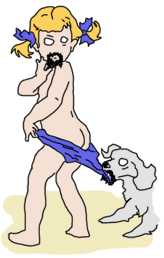
\includegraphics[width=0.3\linewidth]{coppertone.png}
\end{figure}
На вопрос <<Что же использовать?>>, \--- ответить довольно сложно. Между вызовами функций и конструкцией \ops{case \ldots of} разница очень невелика. На самом деле на низком уровне они реализованы одинаково, поэтому с точки зрения производительности они ничем не отличаются. Различия появляются, когда обрабатывается более чем один аргумент: \ops{function(A,B) -> \ldots end.} может использовать стражи, чтобы сопоставлять  с образцом A и B, тогда как case выражение было бы необходимо сформулировать приблизительно следующим образом:
\begin{lstlisting}[style=erlang]
case {A,B} of
    Pattern Guards -> ...
end.
\end{lstlisting}

Такая форма редко встречается и наверняка застанет читателя врасплох. В похожих ситуациях правильнее было бы использовать вызов функции. С другой стороны, функция \ops{insert/2}, которую мы записали ранее, определённо выглядит яснее в своём текущем виде, без прямого вызова функции, которая проходит по веткам \ops{true} или \ops{false}.

Следующий вопрос: зачем тогда вообще использовать \ops{if}, если \ops{case} и функции достаточно гибки, чтобы реализовать \ops{if} посредством стражей? За \ops{if} стоит простая логика: эта конструкция была добавлена в язык, чтобы иметь возможность использовать стражи, не описывая сопоставления с образцом, когда в них нет необходимости.

Конечно же, всё это относится больше к индивидуальным предпочтениям. Определённого ответа на этот вопрос не существует. Эта тема до сих пор время от времени обсуждается сообществом Erlang. Если ваш код прост для понимания, никто вас бить не будет, какой бы путь вы не избрали. Как однажды сказал Ward Cunningham: <<Код можно считать ясным, когда вы смотрите на подпрограмму, и она выглядит приблизительно так, как вы и ожидали.>>

\chapter{Типы (или отсутствие таковых)}
\label{types-or-lack-thereof}
\section{Типизация сильная, как динамит}
\label{dynamite-strong-typing}
Как вы, вероятно, заметили во время ввода примеров из \ref{starting-out-for-real}, а потом модулей и функций из \ref{modules}~и \ref{syntax-in-functions}, нам не нужно было вводить тип переменной или тип функции.
При сопоставлении с образцом нашему коду не нужно было знать, с чем производится сопоставление.
Кортеж \ops{\{X,Y\}} с одинаковым успехом можно сопоставить как с \ops{\{atom, 123\}}, так и с \ops{\{``A string'', <<``binary stuff!''>>\}}, \ops{\{2.0, [``strings'', ``and'', atoms]\}} или вообще с чем угодно.

При неудачном сопоставлении просто генерировалась ошибка, но она генерировалась только во время исполнения кода.
Причина этого \--- \emph{динамическая типизация} в языке Erlang.
Каждая ошибка ловится во время исполнения.
Если исполнение кода потенциально может закончиться аварией, то компилятор об этом не всегда будет истошно вопить, как в примере \ops{``llama + 5''} из главы \ref{starting-out-for-real}.

\begin{figure}[h!]
    \centering
    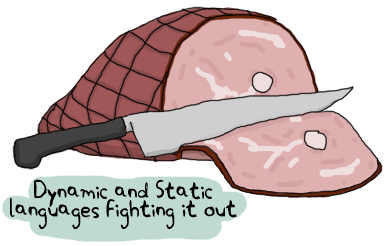
\includegraphics[width=0.4\textwidth]{ham.png}
\end{figure} 
Одной из классических точек трения между сторонниками статической и динамической типизации является безопасность програмного обеспечения.
Очень часто насаждается мысль, что хорошая статическая система типизации, за соблюдением которой с усердием следят компиляторы, будет ловить большинство ошибок ещё до того как код начнёт исполняться.
Поэтому языки со статической типизацией считаются более надёжными, чем их динамические собратья.
Хотя для многих динамических языков это действительно так, но к Erlang это относится не в полной мере, и его послужной список это подтверждает.
Лучшим примером служит степень готовности к обслуживанию (availability) \emph{девять девяток} (99.9999999\%), которая обеспечивается коммутаторами \href{http://www.erlang.se/publications/Ulf_Wiger.pdf}{Ericsson AXD 301 ATM}.
Количество строк Erlang\--кода для этих устройств \--- свыше 1 миллиона.
Обратите внимание \--- этот факт не свидетельствует о том, что ни один из компонентов системы, написанной на Erlang, не давал сбой.
Это означает, что коммутатор как единая система был готов к работе 99.9999999\% времени, включая запланированные перерывы.
Отчасти это заслуга проектировщиков, которые в разработке Erlang руководствовались идеей, что сбой в одной из компонент не должен влиять на всю систему.
При этом учитываются ошибки, которые допускает программист, сбои оборудования или сети.
Язык содержит средства, позволяющие распределять программы на различные узлы, обрабатывать непредвиденные ошибки и \emph{никогда} не останавливаться.

Иначе говоря, в то время как большинство языков и систем типизации стараются избавить программы от ошибок, Erlang использует стратегию, согласно которой считается, что ошибки будут возникать в любом случае, и старается эти случаи предотвратить.
Система динамической типизации в Erlang \--- не преграда для надёжности и безопасности программ.
Всё сказанное мной напоминает речи проповедника, но в последующих главах вы увидите как это происходит.\\
\colorbox{lgray}
{
    \begin{minipage}{\linewidth}
\textbf{Замечание:} динамическая типизация в ретроспективе была избрана по простой причине.
Люди, которые занимались реализацией Erlang, в большинстве своём имели опыт программирования на языках с динамической типизацией, и поэтому динамическая типизация в Erlang была для них самым естественным выбором.
    \end{minipage}
}

Кроме того, Erlang \--- язык с сильной типизацией.
Языки со слабой типизацией производят неявные преобразования типов между термами.
Если бы Erlang был языком со слабой типизацией, то мы, вероятно, смогли бы исполнить операцию \ops{6 = 5 + ''1''}.
В действительности будет выброшено исключение, которое сообщает о неверных аргументах:
\begin{lstlisting}[style=erlang]
1> 6 + "1".
** exception error: bad argument in an arithmetic expression
    in operator  +/2
        called as 6 + "1"
\end{lstlisting}

Конечно же, есть случаи, когда вам хотелось бы преобразовать один вид данных в другой.
Например, привести обычный строковый тип к битовым строкам на время хранения, или целое значение привести к числу с плавающей запятой.
Для таких ситуаций Стандартная библиотека Erlang предлагает множество функций.
\section{Преобразование типов}
\label{type-conversions}
Как и многие языки, Erlang меняет тип терма посредством приведения его к другому типу.
Для этого применяются встроенные функции, поскольку многие преобразования невозможно реализовать на чистом Erlang.
Каждая такая функция имеет форму <тип>\_to\_<тип> и находится в модуле \ops{erlang}.
Вот некоторые из этих функций:
\begin{lstlisting}[style=erlang]
1> erlang:list_to_integer("54").
54
2> erlang:integer_to_list(54).
"54"
3> erlang:list_to_integer("54.32").
** exception error: bad argument
    in function  list_to_integer/1
        called as list_to_integer("54.32")
4> erlang:list_to_float("54.32").
54.32
5> erlang:atom_to_list(true).
"true"
6> erlang:list_to_bitstring("hi there").
<<"hi there">>
7> erlang:bitstring_to_list(<<"hi there">>).
"hi there"
\end{lstlisting}

И так далее.
Здесь мы сталкиваемся с неприятной особенностью языка.
Для именования функций используется схема <тип>\_to\_<тип>, поэтому при добавлении нового типа в язык приходится добавлять множество встроенных функций!
Вот их полный список:\\
\ops{atom\_to\_binary/2, atom\_to\_list/1, binary\_to\_atom/2}\\
\ops{binary\_to\_existing\_atom/2, binary\_to\_list/1,}\\
\ops{bitstring\_to\_list/1, binary\_to\_term/1, float\_to\_list/1,}\\
\ops{fun\_to\_list/1, integer\_to\_list/1, integer\_to\_list/2,}\\
\ops{iolist\_to\_binary/1, iolist\_to\_atom/1, list\_to\_atom/1,}\\
\ops{list\_to\_binary/1, list\_to\_bitstring/1,}\\
\ops{list\_to\_existing\_atom/1, list\_to\_float/1, list\_to\_integer/2,}\\
\ops{list\_to\_pid/1, list\_to\_tuple/1, pid\_to\_list/1,}\\
\ops{port\_to\_list/1, ref\_to\_list/1, term\_to\_binary/1,}\\
\ops{term\_to\_binary/2 и tuple\_to\_list/1.}

Многовато функций.
Большинство из них, если не все, мы увидим в этой книге.
Впрочем, все они нам вряд ли понадобятся.
\section{Охрана типа данных}
\label{to-guard-a-data-type}
Базовые типы Erlang просто заметить: у кортежей есть фигурные скобки, у списков \--- квадратные, строки заключены в двойные кавычки и т.д.
Поэтому определённый тип данных можно использовать в сопоставлении с образцом: функция \ops{head/1}, которая принимает в качестве аргумента список, может принимать списки потому, что для других типов не сработало бы сопоставление (\ops{[H|\_]}).
\begin{figure}[h!]
    \centering
    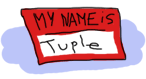
\includegraphics[width=0.3\textwidth]{my-name-is.png}
\end{figure} 

Тем не менее, у нас уже возникали проблемы с числовыми значениями, для которых мы не могли задавать диапазоны.
Для решения этой проблемы мы использовали стражи в функциях, которые были связаны с температурой, водительским возрастом и т.д.
Перед нами встаёт ещё одно препятствие.
Как нам записать страж, который применил бы сопоставление с образцом к данным лишь одного определённого типа, такого как числа, атомы или битовые строки?

Для решения этой задачи предназначены функции, которые возвращают истину, если переданный им аргумент имеет верный тип, и ложь в противоположном случае.
Они составляют группу функций, которые допускаются в охранных выражениях и называются <<встроенными функциями проверки типов>>:
\begin{lstlisting}[style=erlang]
is_atom/1           is_binary/1        
is_bitstring/1      is_boolean/1        is_builtin/3       
is_float/1          is_function/1       is_function/2      
is_integer/1        is_list/1           is_number/1        
is_pid/1            is_port/1           is_record/2        
is_record/3         is_reference/1      is_tuple/1        
\end{lstlisting}

Их можно использовать, как и любое другое охранное выражение, в любом месте, где допускается охранное выражение.
Вы, вероятно, задаёте себе вопрос: почему функция просто не возвращает тип терма, который ей передали (что\--то вроде \ops{type\_of(X) -> Type}).
Ответ прост.
Erlang концентрируется на программировании для корректных ситуаций: вы составляете программу только для событий, которые точно должны произойти, для событий, которые вы ожидаете.
Всё прочее должно как можно раньше вызвать ошибку.
Может быть это покажется абсурдом, но объяснения, которые вы получите в главе \ref{errors-and-exceptions}, я надеюсь, прояснят ситуацию.
А пока что просто поверьте мне на слово.\\
\colorbox{lgray}
{
    \begin{minipage}{\linewidth}
\textbf{Замечание:} встроенные функции проверки типов более чем на половину состоят из инструкций, которые можно использовать в охранных выражениях.
Остальные функции также являются встроенными, но не относятся к функциям проверки типов.
Среди них:\\
\ops{abs(Number), bit\_size(Bitstring), byte\_size(Bitstring),}
\ops{element(N, Tuple), float(Term), hd(List), length(List),}
\ops{node(), node(Pid|Ref|Port), round(Number), self(),}
\ops{size(Tuple|Bitstring), tl(List), trunc(Number), tuple\_size(Tuple).}\\
Функции \ops{node/1} и \ops{self/0} принадлежат к распределённым средствам Erlang и разделу процессов/акторов.
Вскоре мы будем их использовать, но до той поры мы ещё должны изучить много других вещей.
    \end{minipage}
}

Может показаться, что структуры данных в Erlang относительно ограничены, но списков и кортежей обычно достаточно для создания других более сложных структур.
Например, узел двоичного дерева можно представить как \ops{\{node, Value, Left, Right\}}, где \emph{Left} и \emph{Right} это или узлы, одинаковые по структуре, или пустые кортежи.
Я мог бы представить информацию о себе в таком виде:
\begin{lstlisting}[style=erlang]
{person, {name, <<"Fred T-H">>},
    {qualities, ["handsome", "smart", "honest", "objective"]},
    {faults, ["liar"]},
    {skills, ["programming", "bass guitar", "underwater breakdancing"]}}.
\end{lstlisting}

Этот пример показывает, как можно получить сложные структуры данных.
Для этого необходимо вложить списки в кортежи, заполнить их данными, и создать функции, которые будут работать с полученной структурой.\\
\colorbox{lgray}
{
    \begin{minipage}{\linewidth}
\textbf{Дополнение:}
в релизе R13B04 появилась встроенная функция \ops{binary\_to\_term/2}, которая позволяет десериализовать данные так же, как это делает \ops{binary\_to\_term/1}, с тем лишь отличием, что вторым аргументом можно передать список опций.
Если передать опцию \ops{[safe]}, то двоичные данные, содержащие неизвестные атомы или \ref{higher-order-functions}~анонимные функции, которые могут привести к исчерпанию памяти, декодированы не будут.
    \end{minipage}
}
\section{Для <<подсевших на систему>> типизации}
\label{for-type-junkies}
Этот раздел предназначен для программистов, которые по той или иной причине не представляют своё существование без статических систем типизации.
Он содержит слегка усложнённую теорию, которая не всем будет ясна.
Я кратко опишу инструменты, которые используются для статического анализа типов в Erlang, определения специализированных типов, и то, как всё это позволяет получить более безопасный код.
Эти средства будут описаны в книге намного позже, потому как они совсем не обязательны для разработки надёжных программ на Erlang.
Так как мы откладываем их рассмотрение на потом, я дам лишь основные сведения об их установке, запуске и т.д.
Повторюсь: этот раздел предназначен для тех, кто действительно не может жить без развитых систем типизации.
\begin{figure}[h!]
    \centering
    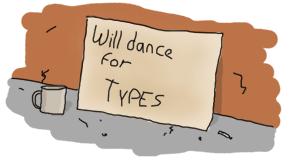
\includegraphics[width=0.4\textwidth]{type-dance.png}
\end{figure} 

На протяжении нескольких лет предпринимались попытки построения системы типов поверх Erlang.
Одна из таких попыток случилась в 1997 году под руководством Simon Marlow, одного из ведущих разработчиков Glasgow Haskell Compiler и Philip Wadler, который работал над проектированием Haskell и внёс свою лепту в теорию, которая лежит в основе монад (\href{http://www.haskell.org/~simonmar/papers/erltc.pdf}{здесь вы можете прочитать работу}, посвящённую упомянутой системе типов).
Joe Armstrong позже \href{http://www.cs.chalmers.se/Cs/Grundutb/Kurser/ppxt/HT2007/general/languages/armstrong-erlang\_history.pdf}{так прокомментировал этот документ}:\\
\colorbox{lgray}
{
    \begin{minipage}{\linewidth}
Однажды мне позвонил Фил и заявил, что а) Erlang необходима система типов, б) он написал непольшой прототип такой системы и в) у него есть возможность взять творческий отпуск, в течение которого он собирался написать систему типов для Erlang, и спрашивал: <<будет ли нам это интересно?>>.
Я ответил: <<Да.>>\\
Phil Wadler и Simon Marlow работали над системой типов больше года, и результаты были опубликованы в [20].
Результаты оказались немного разочаровывающими.
Начнём с того, что на соответствие типов можно было проверять не весь язык, а лишь его подмножество.
Большим упущением было отсутствие типизированных процессов и отсутствие проверки типов для сообщений, пересылаемых между процессами.
    \end{minipage}
}

Процессы и сообщения относятся к основным средствам Erlang.
Может быть именно поэтому система так никогда и не была внедрена.
Были и другие неудачные попытки типизировать Erlang.
В результате усилий проекта HiPE (попытка увеличить производительность Erlang) появился Dialyzer, инструмент статического анализа, который используется до сих пор.
Он имеет свой собственный механизм вывода типов (type inference).

Система типов, которая в нём используется, основана на успешных типизациях (success typings) \--- концепции, которая отличается от системы типов Hindley\--Milner или мягкой типизации (soft\--typing).
Концепция успешной типизации проста: метод определения типов не пытается найти точный тип каждого выражения, но он гарантирует, что выведенные им типы точны, и что ошибки типов, которые он находит, действительно являются ошибками.

В качестве примера лучше всего привести реализацию функции \ops{and}, которая обычно принимает два булевых значения и возвращает 'true', если оба параметра истинны, иначе возвращается 'false'.
В системе типов Haskell это можно записать как \ops{and :: bool -> bool -> bool}.
Если бы нужно было реализовать функцию \ops{and} на Erlang, то это можно было бы сделать следующим образом:
\begin{lstlisting}[style=erlang]
and(false, _) -> false;
and(_, false) -> false;
and(true,true) -> true.
\end{lstlisting}

После применения метода успешной типизации, был бы выведен тип \ops{and(\_,\_) -> bool()}, где \_ означает <<любое значение>>.
Причина появления такого типа проста: при вызыве функции с аргументами \ops{false} и \ops{42}, будет возвращён результат 'false'.
Использование шаблона подстановки \ops{\strut\_} в сопоставлении с образцом привело к тому, что для работы функции достаточно передать хотя бы один аргумент, который равен 'false'.
У системы типов ML случился бы припадок (а у её пользователей сердечный приступ), если бы вы вызвали функцию таким образом.
Но не у Erlang.
В этих строках появится больше смысла, если вы решите прочитать документ про \href{http://www.it.uu.se/research/group/hipe/papers/succ\_types.pdf}{реализацию успешной типизации}, в котором объясняется логика такого поведения.
Я призываю каждого наркозависимого от типов прочитать эту статью.
Она представляет собой интересное и полезное описание реализации метода.

Подробности процесса определения типов и аннотирования функций описаны в Предложении об Улучшении Erlang №8 (\href{http://www.erlang.org/eeps/eep-0008.html}{EEP8}).
Если вас заинтересовало использование успешной типизации в Erlang, взгляните на \href{http://user.it.uu.se/~tobiasl/publications/typer.pdf}{приложение TypEr} и Dialyzer.
Оба входят в стандартный дистрибутив.
Чтобы ими воспользоваться, введите \ops{\$ typer --help} и \ops{\$ dialyzer --help} (для Windows команды \ops{typer.exe --help} и \ops{dialyzer --help}, если они доступны из текущей директории).

TypEr используется для аннотации типов функций.
Запуск TypEr для этой маленькой \href{http://learnyousomeerlang.com/static/erlang/fifo.erl}{реализации FIFO очереди} генерирует следующее описание типов:
\begin{lstlisting}[style=erlang]
%% File: fifo.erl
%% --------------
-spec new() -> {'fifo',[],[]}.
-spec push({'fifo',_,_},_) -> {'fifo',nonempty_maybe_improper_list(),_}.
-spec pop({'fifo',_,maybe_improper_list()}) -> {_,{'fifo',_,_}}.
-spec empty({'fifo',_,_}) -> bool().
\end{lstlisting}

Что, в целом, верно.
Improper списки лучше не использовать, так как с ними не работает функция \ops{lists:reverse/1}, а кто\--нибудь всё\--таки может попытаться протолкнуть такой список, минуя интерфейс модуля.
В этом случае функции \ops{push/2} и \ops{pop/2} всё\--таки отработают несколько вызовов, а затем будет выброшено исключение.
Поэтому нам необходимо добавить стражи, либо вручную оптимизировать определения типов.
Предположим, что мы добавили в модуль сигнатуру\\
\ops{-spec push(\{fifo,list(),list()\},\_) -> \{fifo,nonempty\_list(),list()\}.}\\
и функцию, которая передаёт improper список для \ops{push/2}.
При сканировании Dialyzer\--ом (который проверяет типы на соответствие), будет выведено сообщение об ошибке <<The call fifo:push({fifo,[1|2],[]},3) breaks the contract '<Type definition here>\'>>.
\begin{figure}[h!]
    \centering
    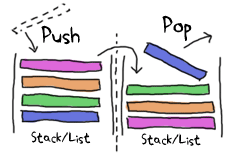
\includegraphics[width=0.4\textwidth]{fifo.png}
\end{figure} 

Dialyzer будет сообщать об ошибках лишь тогда, когда код будет нарушать работу другого кода, и эти сообщения, скорее всего, будут верными (он также будет сообщать и о других проблемах, например о ветках кода, до которых никогда не дойдёт исполнение или об общем рассогласовании).
При помощи Dialyzer\--а можно также анализировать полиморфные типы данных.
Функцию \ops{hd()} можно описать выражением \ops{-spec([A]) -> A.} и корректно проанализировать, впрочем программисты на Erlang редко используют этот синтаксис описания типов.\\
\colorbox{lorange}
{
    \begin{minipage}{\linewidth}
        \textbf{Не забывайтесь:}\\
Dialyzer и TypEr не обрабатывают классы типов с конструкторами, типы первого порядка и рекурсивные типы.
Типы в Erlang \--- это лишь аннотация, которая никак не влияет на компиляцию и не ограничивает её, кроме ситуаций, когда вы сами накладываете эти ограничения.
Программа проверки типов никогда не сообщит вам, что в приложении, которое работает прямо сейчас (или исполняется уже на протяжении двух лет), есть ошибка типов, которая никак себя не проявляет во время исполнения (корректное исполнение не говорит о том, что в коде нет ошибок\ldots)\\
Неплохо было бы иметь возможность создания рекурсивных типов, но они вряд ли когда\--нибудь появятся для TypEr и Dialyzer в текущем состоянии (объяснение можно найти в статье, указанной выше).
На текущий момент можно лишь вручную симулировать рекурсивные типы добавлением нескольких уровней вложенности.\\
Конечно же, это нельзя назвать  всеобъемлющей системой типов, сравнимой со строгостью и мощью систем типизации в Scala, Haskell или OCaml.
Предупреждения и сообщения об ошибках обычно слегка запутаны и не всегда ясны пользователю.
Но если вы просто не можете существовать в мире динамического языка или жаждете дополнительной надёжности \--- это решение предлагает очень неплохой компромисс.
Относитесь к нему как к инструменту в вашем арсенале, не более.
    \end{minipage}
}
\colorbox{lgray}
{
    \begin{minipage}{\linewidth}
\textbf{Дополнение:}\\
Начиная с версии R13B04, в Dialyzer была добавлена экспериментальная возможность работы с рекурсивными типами.
Этот факт делает предыдущий раздел отчасти неверным.
Стыд мне и срам.\\
Также заметьте, что \href{http://erlang.org/doc/reference\_manual/typespec.html}{документация, описывающая типы, стала официальной} (хотя она и может в будущем измениться) и более полной, чем в EEP8.
    \end{minipage}
}

\chapter{Рекурсия}
\label{recursion}
\section{Привет, рекурсия!}
\begin{wrapfigure}{r}{0.4\linewidth}
    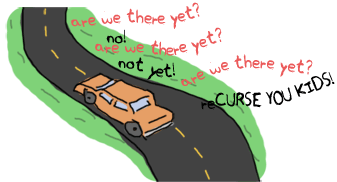
\includegraphics[width=1\linewidth]{reCURSE.png}
\end{wrapfigure}
Некоторые читатели, знакомые с императивными и объектно\--ориентированными языками программирования, должно быть, недоумевают, почему до сих пор не были показаны циклы.
Ответить на это можно вопросом: <<Что такое цикл?>>
По правде говоря, функциональные языки программирования обычно не предлагают средства построения циклов, такие как \ops{for} и \ops{while}.
Вместо них программисты\--функциональщики полагаются на незамысловатую концепцию, именуемую \emph{рекурсией}.

Вы, должно быть, помните как во вводной главе объяснялись неизменяемые переменные.
Если не помните, то уделите им \ref{invariable-variables}~ещё немного внимания!
Рекурсию тоже можно объяснить при помощи математических концепций и функций.
Хорошим примером функции, которую можно выразить в рекурсивном виде, может послужить примитивная функция вычисления факториала.
Факториал числа \emph{n} это произведение последовательности \ops{$1\times 2\times3\times\ldots\times\emph{n}$} или \ops{$n\times n-1 \times n-2\times\ldots\times 1$}.
Например, факториал числа 3 равен \ops{$3! = 3 \times 2 \times 1 = 6$}.
Факториал 4 равен \ops{$4! = 4 \times 3 \times 2 \times 1 = 24$}.
Эту функцию можно выразить при помощи математической записи в следующем виде:
\[
n! =
  \begin{cases}
   1           & \text{if } x = 0 \\
   n((n - 1)!) & \text{if } x < 0
  \end{cases}
\]

Это означает, что если n равно 0, то в качестве результата возвращается 1.
Для любого значения больше 0 возвращается \emph{n} умноженное на факториал \ops{n - 1}, значение которого тоже раскрывается, до тех пор, пока не достигнет 1.
\begin{align*}
4! &= 4 \times 3! \\
4! &= 4 \times 3 \times 2! \\
4! &= 4 \times 3 \times 2 \times 1! \\
4! &= 4 \times 3 \times 2 \times 1 \times 1 \\
\end{align*}

Как же записать такую математическую функцию на Erlang? Очень просто.
Взгляните на части записи: \ops{n!}, 1 и \ops{n((n-1)!)}, а затем на \ops{if}\--ы.
Мы можем различить имя функции (\ops{n!}), стражей (им соответствуют \ops{if}\--ы) и тело функции (1 и \ops{n((n-1)!)}).
Мы переименуем \ops{n!} в \ops{fac(N)}, чтобы немного ограничить наш синтаксис, и получим следующее:
\begin{lstlisting}[style=erlang]
-module(recursive).
-export([fac/1]).
 
fac(N) when N == 0 -> 1;
fac(N) when N > 0  -> N*fac(N-1).
\end{lstlisting}

Вот и готова наша функция для вычисления факториала!
Она очень похожа на математическое определение.
Применяя сопоставление с образцом, мы можем немного сократить её объявление:
\begin{lstlisting}[style=erlang]
fac(0) -> 1;
fac(N) when N > 0 -> N*fac(N-1).
\end{lstlisting}

Для математического определения, которое рекурсивно по своей природе, трансляция на Erlang происходит просто и быстро.
Мы записали цикл!
Определение рекурсивной функции можно сократить до <<функция, которая вызывает саму себя>>.
Также нам необходимо определить условие остановки вычислений (это называется базовым случаем), так как без такого условия мы будем находиться в цикле бесконечно.
В нашем примере условие остановки \--- это состояние, когда \emph{n} равно 0.
В момент, когда это условие истинно, мы перестаём вызывать функцию, и её исполнение прекращается. 
\section{Длина}
\label{length}
Попробуем перейти к более практичным вещам.
Напишем функцию, которая считает количество элементов, содержащихся в списке.
Сразу же ясно, что нам понадобится:\\
\begin{itemize}
\item базовый случай;
\item функция, которая вызывает сама себя;
\item список, к которому мы применим нашу функцию.
\end{itemize}

Мне кажется, что для большинства рекурсивных функций проще всего сначала записать базовый случай.
Что представляет собой самый простой входящий параметр, для которого мы можем найти длину?
Это, конечно же, пустой список, длина которого равна 0.
Поэтому запомним, что \ops{[] = 0}.
Следующий по простоте список имеет длину 1: \ops{[\_] = 1}.
Похоже, у нас есть всё необходимое, чтобы записать определение нашей функции:
\begin{lstlisting}[style=erlang]
len([]) -> 0;
len([_]) -> 1.
\end{lstlisting}

Прекрасно!
Мы можем подсчитать длину списка, если он содержит 0 либо 1 элемент!
Очень полезная возможность.
Правда, пользы в ней не так много, потому что ей не хватает рекурсивности.
Это приводит нас к самому сложному моменту: нам необходимо расширить функцию таким образом, чтобы она вызывала сама себя для списков с длиной больше 0 и 1.
Ранее мы \ref{lists}~упоминали, что списки определяются рекурсивно как \ops{[1 | [2| \ldots [n| []]]]}.
Это означает, что мы можем использовать образец \ops{[H|T]} для сопоставления со списками одного и более элементов, так как список с одним элементом можно определить как \ops{[X|[]]}, а список с двумя элементами как \ops{[X|[Y|[]]]}.
Обратите внимание, что второй элемент сам является списком.
Поэтому нам нужно посчитать лишь первый элемент, а потом функция может вызвать себя для второго элемента.
Если учесть, что каждый элемент в списке прибавляет к длине 1, то функцию можно переписать в следующем виде:
\begin{lstlisting}[style=erlang]
len([]) -> 0;
len([_|T]) -> 1 + len(T).
\end{lstlisting}

Вот у нас и появилась рекурсивная функция, которая определяет длину списка.
Давайте посмотрим как она будет вести себя при исполнении. Попробуем применить её, например, к списку \ops{[1,2,3,4]}: \begin{align*}
len([1,2,3,4]) &= len([1 | [2,3,4])\\
&= 1 + len([2 | [3,4,]])\\
&= 1 + 1 + len([3 | [4]])\\
&= 1 + 1 + 1 + len([4 | []])\\
&= 1 + 1 + 1 + 1 + len([])\\
&= 1 + 1 + 1 + 1 + 0\\
&= 1 + 1 + 1 + 1\\
&= 1 + 1 + 2\\
&= 1 + 3\\
&= 4
\end{align*}
Мы получили верный результат.
Поздравляю вас с первой полезной рекурсивной функцией на Erlang!
\section{Длина хвостовой рекурсии}
\label{length-of-a-tail-recursion}

\begin{wrapfigure}{l}{0.4\linewidth}
    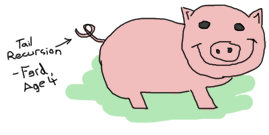
\includegraphics[width=1\linewidth]{tail-recursion.png}
\end{wrapfigure}
Возможно, вы заметили, что для списка из четырёх термов, мы разложили вызов нашей функций на цепь из пяти операций суммирования.
Хотя этот принцип хорошо работает для коротких списков, он может создать проблемы для случая, когда ваш список содержит несколько миллионов значений.
Для такого простого вычисления совсем не обязательно хранить в памяти миллионы чисел.
Это слишком расточительно, к тому же, есть способ получше.
Познакомьтесь с \emph{хвостовой рекурсией}.

Хвостовая рекурсия \--- это способ трансформации вышеописанного линейного процесса (который растёт прямо пропорционально количеству элементов) в итеративный (в котором никакого роста нет вообще).
Чтобы вызов функции стал хвостовым, он должен быть <<одиночным>>.
Здесь необходимо пояснить: наши предыдущие вызовы росли из\--за того, что результат первого вызова зависел от вычисления второго.
Чтобы найти ответ для \ops{1 + len(Rest)}, необходимо вычислить результат \ops{len(Rest)}.
А для вычисления \ops{len(Rest)}, в свою очередь, понадобится найти результат ещё одного вызова функции.
Операции суммирования будут накапливаться до тех пор, пока не будет найден результат последней, и только после этого можно будет вычислить конечный результат.
Хвостовая рекурсия позволяет избавиться от этого накопления посредством вычисления операций по мере их возникновения.

Чтобы этого добиться, нам необходимо завести временную переменную и передавать её при каждом вызове функции в качестве дополнительного параметра.
Я проиллюстрирую эту концепцию при помощи функции вычисления факториала.
На этот раз определим её с использованием хвостовой рекурсии.
Вышеупомянутую временную переменную иногда называют \emph{аккумулятором}.
Для ограничения роста вызовов нашей функции, мы сохраняем в аккумуляторе результаты вычислений, по мере того как они происходят:
\begin{lstlisting}[style=erlang]
tail_fac(N) -> tail_fac(N,1).
 
tail_fac(0,Acc) -> Acc;
tail_fac(N,Acc) when N > 0 -> tail_fac(N-1,N*Acc).
\end{lstlisting}

Я определил две функции \ops{tail\_fac/1} и \ops{tail\_fac/2}.
Сделал я это по причине того, что Erlang не позволяет указывать для параметров значения по умолчанию (функции c разной арностью, которые имеют одинаковые имена \--- это разные функции), поэтому мы создаём аналогичный эффект вручную.
В данном случае \ops{tail\_fac/1} реализует абстракцию поверх функции \ops{tail\_fac/2}, которая использует хвостовую рекурсию.
Никого не интересуют детали реализации скрытого аккумулятора, который использует \ops{tail\_fac/2}, поэтому мы будем экспортировать из модуля лишь \ops{tail\_fac/1}.
Исполнение функции можно записать в следующем виде:
\begin{align*}
tail\_fac(4) &= tail\_fac(4,1)\\
tail\_fac(4,1) &= tail\_fac(4-1, 4*1)\\
tail\_fac(3,4) &= tail\_fac(3-1, 3*4)\\
tail\_fac(2,12) &= tail\_fac(2-1,2*12)\\
tail\_fac(1,24) &= tail\_fac(1-1, 1*24)\\
tail\_fac(0,24) &= 24
\end{align*}

Видите разницу?
Теперь нам не нужно держать в памяти одновременно более двух термов.
Количество места, выделяемого под хранение данных, не меняется.
Для вычисления факториала числа 4 понадобится столько же места, сколько для вычисления факториала 1000000 (если не учитывать, что 4! занимает в числовом представлении намного меньше места, чем 1000000!).

Теперь, когда вы видели функцию вычисления факториала с использованием хвостовой рекурсии, вам, наверняка, ясно как этот шаблон можно применить к нашей функции \ops{len/1}.
Необходимо лишь сделать так, чтобы к результату рекурсивного вызова больше не применялись никакие операции.
Для тех, кто любит визуальные примеры, представьте, что вы помещаете операцию \ops{+1} внутрь вызова функции путём добавления к параметру:
\begin{lstlisting}[style=erlang]
len([]) -> 0;
len([_|T]) -> 1 + len(T).
\end{lstlisting}
принимает вид:
\begin{lstlisting}[style=erlang]
tail_len(L) -> tail_len(L,0).
 
tail_len([], Acc) -> Acc;
tail_len([_|T], Acc) -> tail_len(T,Acc+1).
\end{lstlisting}

Теперь ваша функция вычисления длины списка использует хвостовую рекурсию.
\section{Снова рекурсивные функции}
\begin{wrapfigure}{l}{0.3\linewidth}
    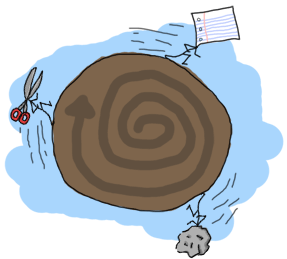
\includegraphics[width=1\linewidth]{rock-paper-scissors.png}
\end{wrapfigure}
Чтобы немного привыкнуть к рекурсивным функциям, мы напишем ещё несколько.
В конце концов, рекурсия \--- это единственный способ организации итераций, который существует в Erlang (кроме списковых выражений), поэтому эту концепцию очень важно понимать.
Это знание будет также полезно для любого другого функционального языка программирования, с которым вы можете столкнуться позже, поэтому запоминайте!

Первая функция, которую мы напишем \--- \ops{duplicate/2}.
Она принимает первым параметром целое число, а вторым \--- произвольный терм.
Затем она создаёт список, который содержит столько копий терма, сколько указано в первом параметре.
Как и ранее, для начала неплохо подумать о базовом случае.
Самое простое, что может сделать функция \ops{duplicate/2}, это повторить что\--либо 0 раз.
Для этого она должна просто возвратить пустой список, не учитывая передаваемый терм.
В любом другом случае мы должны пытаться добраться до базового путём рекурсивного вызова функции.
Вдобавок, мы запретим целому параметру принимать отрицательные значения, потому что нельзя повторить что\--либо \ops{-n} раз:
\begin{lstlisting}[style=erlang]
duplicate(0,_) ->
    [];
duplicate(N,Term) when N > 0 ->
    [Term|duplicate(N-1,Term)].
\end{lstlisting}

Как только мы определили основную рекурсивную функцию, её становится проще записать в виде, который использует хвостовую рекурсию.
Делается это путём перемещения операции создания списка во временную переменную:
\begin{lstlisting}[style=erlang]
tail_duplicate(N,Term) ->
    tail_duplicate(N,Term,[]).
 
tail_duplicate(0,_,List) ->
    List;
tail_duplicate(N,Term,List) when N > 0 ->
    tail_duplicate(N-1, Term, [Term|List]).
\end{lstlisting}

Получилось!
Теперь я хотел бы немного изменить предмет обсуждения, чтобы обозначить связь между хвостовой рекурсией и циклом while.
Наша функция \ops{tail\_duplicate/2} содержит все части, которые присущи циклу while.
Если бы мы представили себе цикл while в выдуманном языке с синтаксисом похожим на Erlang, то наша функция могла бы выглядеть следующим образом:
\begin{lstlisting}[style=erlang]
function(N, Term) ->
    while N > 0 ->
        List = [Term|List],
        N = N-1
    end,
    List.
\end{lstlisting}

Обратите внимание, что все элементы цикла присутствуют как в воображаемом языке, так и в Erlang.
Отличается лишь их расположение.
Это показывает, что правильно написанная функция, использующая хвостовую рекурсию, подобна итеративному процессу, такому как цикл while.

Есть также ещё одно интересное свойство, которое мы <<откроем>> путём сравнении рекурсивной функции и функции с хвостовой рекурсией.
Мы напишем функцию \ops{reverse/1}, которая будет разворачивать список термов задом\--наперёд.
Базовым случаем в этой функции является пустой список, для которого разворачивать нечего.
Для пустого списка мы можем просто вернуть пустой список.
В любой другой ситуации функция должна сходиться к базовому случаю, вызывая саму себя, как это было в \ops{duplicate/2}.
Наша функция будет перебирать элементы списка при помощи сопоставления с образцом \ops{H|T]}, а потом добавлять \emph{H} в конец списка:
\begin{lstlisting}[style=erlang]
reverse([]) -> [];
reverse([H|T]) -> reverse(T)++[H].
\end{lstlisting}

Для длинных списков это может оказаться настоящим кошмаром: помимо проблемы наслаивания функций добавления, нам придётся для каждой операции добавления в конец списка проходить список полностью от начала до конца!
Визуально это можно представить как:
\begin{align*}
reverse([1,2,3,4]) &= [4]++[3]++[2]++[1]\\
&= [4,3]++[2]++[1]\\
&= [4,3,2]++[1]\\
&= [4,3,2,1]\\
\end{align*}

На помощь к нам приходит хвостовая рекурсия.
Мы будем добавлять к аккумулятору новый головной элемент на каждой итерации.
Это автоматически развернёт список в противоположном направлении.
Посмотрим на реализацию:
\begin{lstlisting}[style=erlang]
tail_reverse(L) -> tail_reverse(L,[]).
 
tail_reverse([],Acc) -> Acc;
tail_reverse([H|T],Acc) -> tail_reverse(T, [H|Acc]).
\end{lstlisting}

Если мы распишем шаги исполнения этой функции, то получим:
\begin{align*}
tail\_reverse([1,2,3,4]) &= tail\_reverse([2,3,4], [1])\\
&= tail\_reverse([3,4,], [2,1])\\
&= tail\_reverse([4], [3,2,1])\\
&= tail\_reverse([], [4,3,2,1])\\
&= [4,3,2,1]
\end{align*}

Можно заметить, что теперь мы посещаем линейное количество элементов.
Наш стек не будет расти, и эффективность выполнения операций добавления элементов в этом случае намного выше!

Реализуем ещё одну функцию \--- \ops{sublist/2}. Она принимает список \emph{L} и целое число \emph{N}, и возвращает первых \emph{N} элементов из списка.
Например, вызов \ops{sublist([1,2,3,4,5,6],3)} возвратит [1,2,3].
И снова базовый случай \--- попытка получить 0 элементов из списка.
Впрочем, будьте осторожны, так как в случае \ops{sublist/2} есть отличия.
Есть и второй базовый случай, в котором передаётся пустой список!
Если мы не сделаем проверку списка на пустоту, то при вызове \ops{recursive:sublist([1],2).} будет выброшена ошибка, хотя в качестве результата мы ожидали получить \ops{[1]}.
Как только мы разобрались с этими проблемами, рекурсивной части функции остаётся лишь пройти по списку, сохраняя элементы до тех пор, пока она не упрётся в один из базовых случаев:
\begin{lstlisting}[style=erlang]
sublist(_,0) -> [];
sublist([],_) -> [];
sublist([H|T],N) when N > 0 -> [H|sublist(T,N-1)].
\end{lstlisting}

Функцию можно привести к форме с использованием хвостовой рекурсии тем же путём, что и прежде:
\begin{lstlisting}[style=erlang]
tail_sublist(L, N) -> tail_sublist(L, N, []).
 
tail_sublist(_, 0, SubList) -> SubList;
tail_sublist([], _, SubList) -> SubList;
tail_sublist([H|T], N, SubList) when N > 0 ->
tail_sublist(T, N-1, [H|SubList]).
\end{lstlisting}

Но в этой функции есть изъян.
Роковой изъян!
Мы используем в качестве аккумулятора список, так же как мы это делали, когда разворачивали список задом\--наперёд.
Если вы сейчас скомпилируете функцию, то вызов \ops{sublist([1,2,3,4,5,6],3)} возвратит не [1,2,3], а [3,2,1].
Поэтому нам нужно взять окончательный результат и развернуть его самостоятельно.
Просто поменяйте вызов \ops{tail\_sublist/2}, а рекурсивную логику оставьте прежней:
\begin{lstlisting}[style=erlang]
tail_sublist(L, N) -> reverse(tail_sublist(L, N, [])).
\end{lstlisting}

Окончательный результат будет упорядочен правильно.
Может показаться, что разворот списка после вызова хвостовой рекурсии \--- напрасная потеря времени, и это отчасти правда (таким образом мы всё равно экономим память).
Вы сможете заметить, что из\--за необходимости разворота, на коротких списках ваш код с использованием обычной рекурсии работает быстрее, чем код с хвостовой рекурсией.
Но по мере увеличения объёма данных, на фоне остальных операций разворачивание списка будет значить всё меньше и меньше.\\
\colorbox{lgray}
{
    \begin{minipage}{\linewidth}
\textbf{Замечание:} вместо собственноручно написанной функции \ops{reverse/1} вы должны использовать \ops{lists:reverse/1}.
Функция так часто использовалась для вызовов с хвостовой рекурсией, что разработчики Erlang решили превратить её во встроенную.
Списки будут разворачиваться чрезвычайно быстро (благодаря тому, что функция написана на языке C), что сделает замедление, которое вносит разворот, менее заметным.
Остальной код в этой главе будет использовать нашу собственную функцию разворота элементов, но больше вы её никогда использовать не должны.
    \end{minipage}
}

Чтобы немного развить тему, мы напишем zip\--функцию.
Такая функция принимает в качестве параметров два списка одинаковой длины и попарно комбинирует их элементы в виде списка кортежей.
Наша функция \ops{zip/2} будет вести себя следующим образом:
\begin{lstlisting}[style=erlang]
1> recursive:zip([a,b,c],[1,2,3]).
[{a,1},{b,2},{c,3}]
\end{lstlisting}

Так как мы хотим, чтобы оба параметра имели одинаковую длину, нашим базовым случаем будет комбинирование двух пустых списков:
\begin{lstlisting}[style=erlang]
zip([],[]) -> [];
zip([X|Xs],[Y|Ys]) -> [{X,Y}|zip(Xs,Ys)].
\end{lstlisting}

Однако, если вы хотите, чтобы функция мягче относилась к параметрам, лучше позволить ей заканчивать обработку, когда опустеет один из списков.
Для такого сценария у вас появится два базовых случая:
\begin{lstlisting}[style=erlang]
lenient_zip([],_) -> [];
lenient_zip(_,[]) -> [];
lenient_zip([X|Xs],[Y|Ys]) -> [{X,Y}|lenient_zip(Xs,Ys)].
\end{lstlisting}

Обратите внимание, что вне зависимости от того, какие мы определяем базовые случаи, рекурсивная часть функции остаётся неизменной.
Я бы посоветовал вам попробовать написать собственные версии \ops{zip/2} и \ops{lenient\_zip/2} с использованием хвостовой рекурсии, чтобы убедиться, что вы полностью понимаете как создаются такие функции.
Хвостовая рекурсия будет одной из центральных концепций, лежащих в основе большого приложения, главный цикл которого будет организован именно таким образом.

Если хотите проверить то, что у вас получилось, взгляните на мою реализацию в \href{http://learnyousomeerlang.com/static/erlang/recursive.erl}{recursive.erl}, а именно на функции \ops{tail\_zip/2} и \ops{tail\_lenient\_zip/3}.
\colorbox{lgray}
{
    \begin{minipage}{\linewidth}
\textbf{Замечание:} хвостовая рекурсия не раздувает используемую память, так как виртуальная машина видит, что рекурсивный вызов происходит из хвостовой позиции (последнее выражение, которое обрабатывает функция), и устраняет текущий стековый кадр.
Эта техника называется оптимизацией хвостового вызова и является специальным случаем более общей оптимизации под названием \emph{оптимизация последнего вызова}.\\
Оптимизация последнего вызова происходит, когда последнее выражение в теле функции является ещё одним вызовом функции.
В этом случае, как и в случае оптимизации хвостовой рекурсии, виртуальная машина Erlang не сохраняет стековый кадр.
Поэтому хвостовая рекурсия возможна между несколькими функциями.
Например, цепь функций \ops{a() -> b(). b() -> c(). c() -> a().} создаст в результате бесконечный цикл, который не приведёт к исчерпанию памяти, так как оптимизация последнего вызова предотвращает переполнение стека.
Этот принцип в сочетании с использованием аккумуляторов делает хвостовую рекурсию полезной техникой.
    \end{minipage}
}
\section{Быстро, сортируй!}
\begin{wrapfigure}{l}{0.4\linewidth}
    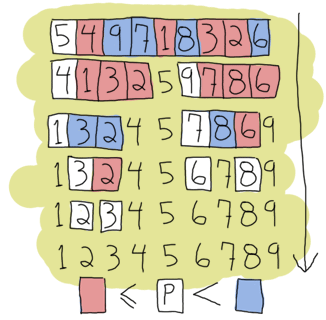
\includegraphics[width=1\linewidth]{quicksort.png}
\end{wrapfigure}
Я могу (и буду) считать, что рекурсия и хвостовая рекурсия вам ясна.
Но просто чтобы в этом убедиться, я приведу более сложный пример \--- реализацию алгоритма быстрой сортировки.
Да, традиционный <<эй, смотри, я могу писать сжатый функциональный код>> канонический пример.
Наивная реализация алгоритма быстой сортировки выбирает первый элемент списка, \emph{опорный элемент}, и перемещает все элементы меньшие, либо равные опорному элементу в новый список, а все элементы больше опорного элемента \--- в другой список.
Затем мы повторяем эту процедуру для полученных списков.
Этот процесс продложается до тех пор, пока для сортировки не останется ничего, кроме пустых списков, которые и станут нашим базовым случаем.
Эта реализация считается простой, потому что более эффективные версии быстрой сортировки будут пытаться выбрать оптимальные опорные элементы с целью ускорения.
Впрочем, в нашем примере это не столь важно.

Нам понадобятся две функции: первая будет разбивать список на части, содержащие меньшие и большие элементы, а вторая будет применять функцию разбиения к новым спискам и соединять их в единое целое.
Для начала мы напишем функцию соединения:
\begin{lstlisting}[style=erlang]
quicksort([]) -> [];
quicksort([Pivot|Rest]) ->
{Smaller, Larger} = partition(Pivot,Rest,[],[]),
quicksort(Smaller) ++ [Pivot] ++ quicksort(Larger).
\end{lstlisting}

Здесь мы видим: базовый случай; список, который разбит при помощи ещё одной функции на части с большими и меньшими элементами; опорный элемент, к которому слева и справа присоединены отсортированные списки.
Этот код отвечает за соединение списков.
Перейдём к функции разбиения:
\begin{lstlisting}[style=erlang]
partition(_,[], Smaller, Larger) -> {Smaller, Larger};
partition(Pivot, [H|T], Smaller, Larger) ->
    if H =< Pivot -> partition(Pivot, T, [H|Smaller], Larger);
        H >  Pivot -> partition(Pivot, T, Smaller, [H|Larger])
    end.
\end{lstlisting}

Теперь функцию быстрой сортировки можно запустить.
Если вы искали в Интернет примеры программ на Erlang, то, скорее всего, наталкивались на другую реализацию быстрой сортировки, ту, которая выглядит проще и легче читается, но использует списковые выражения.
Их легко можно применить в месте, где создаются новые списки, в функции \ops{partition/4}:
\begin{lstlisting}[style=erlang]
lc_quicksort([]) -> [];
lc_quicksort([Pivot|Rest]) ->
    lc_quicksort([Smaller || Smaller <- Rest, Smaller =< Pivot])
    ++ [Pivot] ++
    lc_quicksort([Larger || Larger <- Rest, Larger > Pivot]).
\end{lstlisting}

Главное отличие этой версии в том, что её код легче читать, но за лёгкость чтения приходится платить тем, что для разбиения списка, необходимо перебрать все его элементы.
В этом проявляется борьба ясности кода против скорости его исполнения.
Но проигрываете в этой борьбе лишь вы, потому что для таких ситуаций уже создана функция \ops{lists:sort/1}.
Используйте лучше её.\\
\colorbox{lorange}
{
    \begin{minipage}{1.0\linewidth}
\textbf{Не забывайтесь:}\\
Выразительность кода хороша для обучения, но не всегда полезна для производительности.
Множество руководств по функциональному программированию ни слова об этом не говорят!
Во\--первых, обеим реализациям, приведённым здесь, приходится неоднократно обрабатывать элементы равные опорному элементу.
Для увеличения эффективности можно было бы возвращать три списка: элементы меньше, больше и равные опорному элементу.\\
Ещё одна проблема связана с тем, что нам необходимо неоднократно проходить по разбитым спискам при их слиянии с опорным элементом.
Можно немного уменьшить накладные расходы, если производить объединение во время разбиения списков на три части.
Тем, кто заинтересовался реализацией, я предлагаю взглянуть на последнюю функцию (\ops{bestest\_qsort/1}) из файла \href{http://learnyousomeerlang.com/static/erlang/recursive.erl}{recursive/erl}.\\
Приятно отметить, что все рассмотренные реализации быстрой сортировки будут работать со списками, содержащими любые типы, даже кортежи или что\--то подобное.
Попробуйте, они работают!
    \end{minipage}
}
\section{Больше чем списки}
\begin{wrapfigure}{l}{0.4\linewidth}
    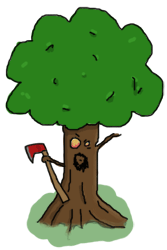
\includegraphics[width=1\linewidth]{tree.png}
\end{wrapfigure}
Читая эту главу, вы, возможно, начинаете думать, что рекурсия в Erlang, главным образом, связана со списками.
Хотя списки и могут служить хорошим примером структуры, которую можно определить через рекурсию, но на ней, конечно, всё не заканчивается.
Мы рассмотрим, для разнообразия, как можно создавать двоичные деревья и считывать из них данные.

Для начала неплохо было бы определить, что такое дерево.
В нашем случае оно снизу доверху состоит из узлов.
Узлы \--- это кортежи, которые содержат ключ, данные связанные с ключом, и два других узла.
Эти два узла мы разделяем на узел с ключом меньшим и большим, чем ключ узла, который их содержит.
И вот появляется рекурсия!
Дерево \--- это узел, который содержит узлы, каждый из которых содержит узлы, которые, в свою очередь, содержат узлы.
Бесконечно это не может продолжаться (у нас нет бесконечного пространства для хранения данных), поэтому мы скажем, что узлы, которые содержатся в наших узлах, также могут быть пустыми.

Кортежи \--- подходящая структура для представления узлов.
Для нашей реализации мы определим такие кортежи как \ops{\{node, \{Key, Value, Smaller, Larger\}\}} (меченый кортеж!), где \emph{Smaller} и \emph{Larger} могут быть другим подобным узлом, или пустым узлом (\ops{\{node, nil\}}.
Более сложные концепции нам не понадобятся.

Начнём создавать модуль для нашей \href{http://learnyousomeerlang.com/static/erlang/tree.erl}{очень простой реализации дерева}.
Первая функция \ops{empty/0} \--- возвращает пустой узел.
Пустой узел \--- это начальная точка нового дерева, которая также называется \emph{корневым узлом}:
\begin{lstlisting}[style=erlang]
-module(tree).
-export([empty/0, insert/3, lookup/2]).
 
empty() -> {node, 'nil'}.
\end{lstlisting}

Мы скрываем реализацию, используя эту функцию, и, затем, инкапсулируем её в одинаковое представление узлов, чтобы пользователю не пришлось задумываться о том, как устроен наш код.
Вся эта информация будет существовать лишь в рамках модуля.
Если вам когда\--либо придёт в голову изменить представление узла \--- вы сможете сделать изменения, не нарушая работу внешнего кода.

Для того, чтобы наполнить дерево содержимым, нам необходимо, для начала, понять, как по нему рекурсивно перемещаться.
Давайте поступим так же, как мы поступали в любом другом примере с рекурсией \--- попытаемся найти базовый случай.
Так как пустое дерево состоит из пустого узла, то, рассуждая логически, нашим базовым случаем будет пустой узел.
Мы сможем добавить новую пару ключ/значение, когда наткнёмся на пустой узел.
В остальных случаях наш код будет ходить по дереву в поисках пустого узла, который можно наполнить данными.

Мы будем искать пустой узел, начиная с корневого узла.
Для этого мы должны использовать знание о том, что \emph{Меньший} и \emph{Больший} узлы позволяют нам определять направление перемещения, сравнивая новый ключ, который необходимо добавить, с ключом текущего узла.
Если новый ключ меньше ключа текущего узла, то мы продолжаем искать пустой узел внутри \emph{Меньшего} узла, и если больше, то внутри \emph{Большего}.
Нельзя забывать ещё об одном случае: что будет, если новый ключ равен ключу текущего узла?
У нас есть две возможности: сгенерировать ошибку, либо заменить значение узла новым.
Здесь мы используем замену.
Все эти рассуждения, заключённые в код, выглядят следующим образом:
\begin{lstlisting}[style=erlang]
insert(Key, Val, {node, 'nil'}) ->
    {node, {Key, Val, {node, 'nil'}, {node, 'nil'}}};
insert(NewKey, NewVal, {node, {Key, Val, Smaller, Larger}}) when NewKey < Key ->
    {node, {Key, Val, insert(NewKey, NewVal, Smaller), Larger}};
insert(NewKey, NewVal, {node, {Key, Val, Smaller, Larger}}) when NewKey > Key ->
    {node, {Key, Val, Smaller, insert(NewKey, NewVal, Larger)}};
insert(Key, Val, {node, {Key, _, Smaller, Larger}}) ->
    {node, {Key, Val, Smaller, Larger}}.
\end{lstlisting}

Обратите внимание, что функция возвращает совершенно новое дерево.
Это характерная черта функциональных языков программирования, в которых присваивание происходит лишь один раз.
Хотя это и может показаться неэффективным, но большая часть структур, которые лежат в основе обеих версий дерева, остаются теми же и используются совместно, а поэтому копируются виртуальной машиной лишь по необходимости.

Для завершения этой демонстрационной реализации дерева, нам необходимо создать функцию \ops{lookup/2}, которая позволит найти значение узла по ключу.
Мы будем использовать принцип, чрезвычайно похожий на тот, который мы использовали при добавлении новых данных в дерево: мы проходим по узлам дерева, шаг за шагом проверяя, что искомый ключ больше, меньше, либо равен ключу текущего узла.
У нас есть два базовых случая: первый \--- когда узел пуст (ключа в дереве нет), и второй \--- когда ключ найден.
Мы не хотим, чтобы наша программа сбоила каждый раз, когда мы ищем ключ, который в дереве отсутствует, а поэтому в такой ситуации мы будем возвращать атом 'undefined'.
В случае удачи, мы возвращаем \ops{\{ok, Value\}}.
Если бы мы просто возвращали \emph{Value}, а искомый узел содержал атом 'undefined', то мы не могли бы понять, было найдено верное значение или нет.
Обёртывание успешно найденных результатов позволяет их легко отличать от неудачных.
Вот реализация функции:
\begin{lstlisting}[style=erlang]
lookup(_, {node, 'nil'}) ->
    undefined;
lookup(Key, {node, {Key, Val, _, _}}) ->
    {ok, Val};
lookup(Key, {node, {NodeKey, _, Smaller, _}}) when Key < NodeKey ->
    lookup(Key, Smaller);
lookup(Key, {node, {_, _, _, Larger}}) ->
    lookup(Key, Larger).
\end{lstlisting}

Всё, мы закончили.
Давайте потестируем нашу структуру \--- напишем небольшую адресную книгу для электронной почты.
Скомпилируйте файл и запустите оболочку:
\begin{lstlisting}[style=erlang]
1> T1 = tree:insert("Jim Woodland", "jim.woodland@gmail.com", tree:empty()).
{node,{"Jim Woodland","jim.woodland@gmail.com",
    {node,nil},
    {node,nil}}}
2> T2 = tree:insert("Mark Anderson", "i.am.a@hotmail.com", T1).
{node,{"Jim Woodland","jim.woodland@gmail.com",
    {node,nil},
    {node,{"Mark Anderson","i.am.a@hotmail.com",
        {node,nil},
        {node,nil}}}}}
3> Addresses = tree:insert("Anita Bath", "abath@someuni.edu", tree:insert("Kevin Robert", "myfairy@yahoo.com", tree:insert("Wilson Longbrow", "longwil@gmail.com", T2))).
{node,{"Jim Woodland","jim.woodland@gmail.com",
    {node,{"Anita Bath","abath@someuni.edu",
        {node,nil},
        {node,nil}}},
    {node,{"Mark Anderson","i.am.a@hotmail.com",
        {node,{"Kevin Robert","myfairy@yahoo.com",
            {node,nil},
            {node,nil}}},
        {node,{"Wilson Longbrow","longwil@gmail.com",
            {node,nil},
            {node,nil}}}}}}}
\end{lstlisting}

Теперь можно поискать адреса с помощью нашей книги:
\begin{lstlisting}[style=erlang]
4> tree:lookup("Anita Bath", Addresses).
{ok, "abath@someuni.edu"}
5> tree:lookup("Jacques Requin", Addresses).
undefined
\end{lstlisting}

На этом мы завершаем рассмотрение примера функциональной адресной книги, построенной при помощи рекурсивной структуры данных отличной от списка!\\
\colorbox{lgray}
{
    \begin{minipage}{\linewidth}
\textbf{Замечание:} наша реализация весьма примитивна: мы не поддерживаем часто используемые операции, такие как удаление узлов или перебалансировка дерева для ускорения последующих операций поиска.
Если вам интересно было бы реализовать и/или изучить эти операции \--- обратитесь к реализации модуля \ops{gb\_trees} (\ops{otp\_src\_R<version>B<revision>/lib/stdlib/src/gb\_trees.erl}).
Кроме того, при работе с деревьями используйте именно этот модуль и не пытайтесь изобрести велосипед.
    \end{minipage}
}
\section{Рекурсивное мышление}
Если вы поняли всё сказанное в этой главе, то рекурсивное мышление, вероятно, начинает становиться частью вашей интуиции.
Главное отличие рекурсивных определений от их императивных аналогов (обычно это циклы while или for) в том, что вместо пошагового выполнения (<<сделай это, потом то, затем вот это, после этого заверши исполнение>>) мы используем декларативный подход (<<если ты получишь такой входящий параметр, сделай это, в противном случае \--- вот это>>).
Такое свойство становится более очевидным при использовании сопоставления с образцом в заголовке функции.

Если вы до сих пор не поняли как работает рекурсия, может быть вам нужно прочитать вот \ref{recursion}~это.

Отбросив шутки в сторону, нужно признать, что иногда рекурсия в сочетании с сопоставлением с образцом \--- это оптимальный способ записи ясных и понятных алгоритмов.
После того как каждая часть задачи поделена на функции, которые не поддаются дальнейшему упрощению, алгоритм превращается в компоновку правильных ответов, получаемых из коротких подпрограмм (что\--то подбное мы делали с быстрой сортировкой).
С обычными циклами можно тоже использовать такой тип мысленной абстракции, но на практике это получается лучше именно с рекурсией.
Ваш опыт может свидетельствовать об ином.

\textbf{А теперь, леди и джентльмены \--- дискуссия автора с самим собой}

\--- Хорошо, кажется я понял рекурсию.
Я понимаю, что она связана с декларативностью, что корни её уходят в математику, как и у неизменяемых переменных. Я понимаю, что в некоторых случаях её проще использовать. Что ещё?

\--- Она имеет регулярную структуру.
Найди базовый случай, запиши его.
Для получения результата нужно, чтобы любой другой случай сходился к одному из базовых.
Так проще записывать функции.

\--- Ага, понял, ты это уже говорил несколько раз.
Я то же самое могу сделать циклами.

\--- Да, можешь.
Не буду отрицать!

\--- Хорошо.
Мне не совсем ясно, зачем ты писал функции, которые не используют хвостовую рекурсию, раз уж они намного хуже тех, что её используют.

\--- А, ну это просто чтобы было легче понять.
Мне показалось, что переход от обычный рекурсии, которая выглядит красивее и проще для понимания, к хвостовой рекурсии, которая теоретически более эффективна, неплохо показал все плюсы и минусы этих подходов.

\--- Хорошо, значит ни для чего кроме обучения они не годятся, я понял.
\begin{wrapfigure}{r}{0.4\linewidth}
    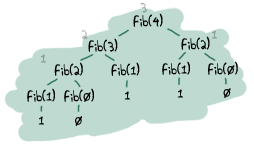
\includegraphics[width=1\linewidth]{fib.png}
\end{wrapfigure}

\--- Это не совсем так.
Разница в производительности между функцией с хвостовой рекурсией и обычной рекурсией будет не сильно заметна.
Хвостовая рекурсия хорошо подходит для функций, которые итерируют бесконечно, например для главных циклов.
Есть также функции, которые порождают очень большой стековый кадр, медленно исполняются и, если их не записывать в виде хвостовой рекурсии, могут рано приводить к аварийному завершению.
Неплохим примером может служить задача вычисления \href{http://en.wikipedia.org/wiki/Fibonacci\_number}{чисел Фибоначчи}, сложность которой растёт экспоненциально, если не решать её в виде итеративного процесса или хвостовой рекурсии.
Также необходимо профилировать написанный код (позже я покажу как это делать, я обещаю), определять и исправлять места, которые замедляют исполнение.

\--- Но циклы \--- это всегда итеративный процесс, проще использовать их и не знать проблем.

\--- Да, но\ldots но\ldots мой прекрасный Erlang\ldots

\--- Ну, зашибись.
Весь сыр\--бор из\--за того, что в Erlang нет <<while>> и <<for>>.
Спасибо большое, я пошёл дальше программировать свой тостер на C!

\--- Погоди\--ка!
У функциональных языков программирования есть и другие возможности!
Кроме шаблона для поиска базовых случаев, который облегчил нам жизнь при написании рекурсивных функций, существует ещё много других шаблонов, которые придумали умные люди.
Благодаря этому необходимость самостоятельно писать рекурсивные функции значительно уменьшается.
Если ты продолжишь занятия, я покажу как строить такие абстракции.
Но для этого нам нужно взять что\--то помощнее.
Позволь мне рассказать о функциях высшего порядка\ldots

\chapter{Функции высшего порядка}
\section{Подбавим функциональщины}
\label{higher-order-functions}
\begin{wrapfigure}{l}{0.3\linewidth}
    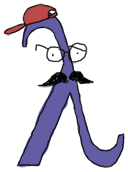
\includegraphics[width=1\linewidth]{lambda.png}
\end{wrapfigure}
Важной частью всех функциональных языков является возможность передачи функции как параметра для другой функции.
Это, в свою очередь, связывает параметр\--функцию с переменной, которую можно использовать внутри функции как любую другую.
Функция, которая может таким способом принимать другие функции, называется функцией высшего порядка.
Функции высшего порядка \--- это мощный способ абстракции и один из лучших инструментов, которым предлагает овладеть Erlang.

Опять же, эта концепция берёт начало в математике, а именно в \href{http://en.wikipedia.org/wiki/Lambda\_calculus}{лямбда\--исчислении}.
Не буду углубляться в детали лямбда\--исчисления, потому что эта теория довольно сложна для понимания, и немного выходит за рамки контекста, который мы рассматриваем.
Тем не менее, я бы кратко охарактеризовал её как систему, в которой всё представлено в виде функций, даже числа.
Так как любая сущность \--- это функция, то в качестве параметров мы должны передавать функциям другие функции и оперировать ими, опять же, при помощи функций!

Ну ладно, наверняка всё сказанное звучит немного странно, поэтому начнём с примера:
\begin{lstlisting}[style=erlang]
-module(hhfuns).
-compile(export_all).
 
one() -> 1.
two() -> 2.
 
add(X,Y) -> X() + Y().
\end{lstlisting}

А теперь откройте оболочку Erlang, скомпилируйте модуль и посмотрите как он работает:
\begin{lstlisting}[style=erlang]
1> c(hhfuns).
{ok, hhfuns}
2> hhfuns:add(one,two).
** exception error: bad function one
    in function  hhfuns:add/2
3> hhfuns:add(1,2).
** exception error: bad function 1
    in function  hhfuns:add/2
4> hhfuns:add(fun hhfuns:one/0, fun hhfuns:two/0).
3
\end{lstlisting}

Не совсем понятно?
Когда разберётесь в принципе работы, сразу станет яснее (всегда так, не правда ли?).
В команде под номером 2 атомы \ops{one} и \ops{two} передаются в функцию \ops{add/2}, которая затем использует оба атома в качестве имён для функций (\ops{X() + Y()}).
Если имена функций записаны без списка параметров, то эти имена интерпретируются как атомы, а атомы не могут быть функциями, поэтому вызов заканчивается неудачей.
По той же причине не удаётся исполнить выражение 3.
Значения 1 и 2 тоже невозможно использовать как функции, а нам нужны именно функции!

Поэтому мы должны использовать новый способ записи, который позволит передавать функции, размещённые за пределами модуля.
Именно такую задачу выполняет \ops{fun Module:Function/Arity}.
Эта строка указывает VM, что та должна взять определённую функцию и привязать её к переменной.

Так что же мы приобретаем, используя функции таким образом?
Для понимания рассмотрим маленький пример.
Мы добавим в модуль \ops{\href{http://learnyousomeerlang.com/static/erlang/hhfuns.erl}{hhfuns}} пару функций, которые будут рекурсивно проходить по списку и прибавлять или вычитать единицу из каждого элемента:
\begin{lstlisting}[style=erlang]
increment([]) -> [];
increment([H|T]) -> [H+1|increment(T)].
 
decrement([]) -> [];
decrement([H|T]) -> [H-1|decrement(T)].
\end{lstlisting}

Видите как эти функции похожи друг на друга?
Они практически делают одно и то же: проходят по списку, применяют к каждому элементу функцию (\ops{+\strut} или \ops{-\strut}) и затем снова вызывают себя.
В этом коде практически ничего не меняется, кроме применяемой функции и рекурсивного вызова.
Для такого рекурсивного вызова над списком, основа всегда остаётся неизменной.
Мы абстрагируем все похожие части в единую функцию (\ops{map/2}), которая будет принимать в качестве аргумента ещё одну функцию:
\begin{lstlisting}[style=erlang]
map(_, []) -> [];
map(F, [H|T]) -> [F(H)|map(F,T)].
 
incr(X) -> X + 1.
decr(X) -> X - 1.
\end{lstlisting}

Которую можно протестировать в оболочке:
\begin{lstlisting}[style=erlang]
1> c(hhfuns).
{ok, hhfuns}
2> L = [1,2,3,4,5].
[1,2,3,4,5]
3> hhfuns:increment(L).
[2,3,4,5,6]
4> hhfuns:decrement(L).
[0,1,2,3,4]
5> hhfuns:map(fun hhfuns:incr/1, L).
[2,3,4,5,6]
6> hhfuns:map(fun hhfuns:decr/1, L).
[0,1,2,3,4]
\end{lstlisting}

В этом примере результат вычислений не меняется, но в результате мы получаем изящную абстракцию!
Каждый раз, когда вы хотите применить функцию к каждому элементу в списке, вам нужно лишь вызвать \ops{map/2} и передать ей в качестве параметра собственную функцию.
Впрочем, было бы утомительно помещать каждую функцию, которую мы хотим передать \ops{map/2} в качестве параметра, в модуль, затем её экспортировать, компилировать и т.д.
В сущности, это просто непрактично.
Нам нужны функции, которые можно было бы определять на ходу\ldots
\section{Анонимные функции}
\label{anonymous-functions}
Анонимные функции, или \emph{funs}, справляются с этой проблемой, позволяя вам декларировать особенный вид функций без необходимости их именования.
Такие функции могут делать практически всё, что умеют обычные функции, кроме рекурсивных вызовов (как бы они их делали? Они же анонимные!) Вот их синтаксис:
\begin{lstlisting}[style=erlang]
fun(Args1) ->
    Expression1, Exp2, ..., ExpN;
    (Args2) ->
    Expression1, Exp2, ..., ExpN;
    (Args3) ->
    Expression1, Exp2, ..., ExpN
end
\end{lstlisting}
А использовать их можно следующим способом:
\begin{lstlisting}[style=erlang]
7> Fn = fun() -> a end.
#Fun<erl_eval.20.67289768>
8> Fn().
a
9> hhfuns:map(fun(X) -> X + 1 end, L).
[2,3,4,5,6]
10> hhfuns:map(fun(X) -> X - 1 end, L).
[0,1,2,3,4]
\end{lstlisting}
Теперь\--то вам, должно быть, становится ясна одна из причин, по которой людям так нравится функциональное программирование: в коде можно создавать абстракции на очень низком уровне.
Поэтому основные концепции, такие как циклы, можно игнорировать, и сконцентрироваться на том, \emph{что} необходимо сделать, вместо того \emph{как} это должно быть сделано.

Анонимные функции и так довольно хороши как абстракции, но в них заключены дополнительные скрытые силы:
\begin{lstlisting}[style=erlang]
11> PrepareAlarm = fun(Room) ->
11>                     io:format("Alarm set in ~s.~n",[Room]),
11>                     fun() -> io:format("Alarm tripped in ~s! Call Batman!~n",[Room]) end
11>                   end.
#Fun<erl_eval.20.67289768>
12> AlarmReady = PrepareAlarm("bathroom").
Alarm set in bathroom.
#Fun<erl_eval.6.13229925>
13> AlarmReady().
Alarm tripped in bathroom! Call Batman!
ok
\end{lstlisting}
\begin{wrapfigure}{r}{0.3\linewidth}
    
\includegraphics[width=1\linewidth]{batman.png}
\end{wrapfigure}
Бэтмэн, оставайся на связи!
Что тут происходит?
Во\--первых, мы декларируем анонимную функцию, которую присваиваем переменной \emph{PrepareAlarm}.
Эта функция ещё не запускалась: её исполнят во время вызова \ops{PrepareAlarm(''bathroom'')}.
В этот момент будет обработан вызов функции \ops{io:format/2}, и на экране отобразится текст ``Alarm set''.
Второе выражение (ещё одна анонимная функция), возвращается вызывающему коду и присваивается переменной \emph{AlarmReady}.
Обратите внимание, что в этой функции значение переменной \emph{Room} берётся из <<родительской>> функции (\emph{PrepareAlarm}).
Этот эффект имеет отношение к концепции \emph{замыканий} (closures).

Чтобы понять замыкания, необходимо понять что такое область действия (контекст).
Область действия функции можно представить как место, в котором хранятся все переменные и их значения.
В функции \ops{base(A) -> B = A + 1.}, \emph{A} и \emph{B} определены в контексте функции \ops{base/1}.
Это означает, что в любом месте функции \ops{base/1} можно обратиться к переменной \emph{A} или \emph{B}, и ожидать, что с ними связано значение.
А когда я говорю ``в любом месте'' \--- я, сынок, не шучу; к анонимным функциям это тоже относится:
\begin{lstlisting}[style=erlang]
base(A) ->
    B = A + 1,
    F = fun() -> A * B end,
    F().
\end{lstlisting}

Переменные B и А всё ещё связаны с областью действия функции \ops{base/1}, поэтому функция F может беспрепятственно к ним обращаться.
Так происходит потому, что F наследует область действия функции \ops{base/1}.
Как и в правилах наследования, которые действуют в реальной жизни, у родителей обычно нет доступа к тому, чем владеют их дети:

\begin{lstlisting}[style=erlang]
base(A) ->
    B = A + 1,
    F = fun() -> C = A * B end,
    F(),
    C.
\end{lstlisting}

В этой версии нашей функции, переменная \emph{B} всё ещё равна \ops{A + 1}, а \emph{F} по прежнему исполняется без проблем.
Но вот переменная \emph{C} существует лишь в контексте анонимной функции \emph{F}.
Когда \ops{base/1} пытается в последней строке обратиться к значению \emph{C}, она натыкается на свободную переменную.
По правде говоря, если бы вы попытались эту функцию скомпилировать, компилятор пришёл бы в бешенство.
Потому что наследование работает лишь в одну сторону.

Важно отметить, что наследуемый контекст повсюду сопровождает анонимную функцию, даже когда её передают другой функции:
\begin{lstlisting}[style=erlang]
a() ->
    Secret = "pony",
    fun() -> Secret end.
 
b(F) ->
    "a/0's password is "++F().
\end{lstlisting}

А если мы её скомпилируем:
\begin{lstlisting}[style=erlang]
14> c(hhfuns).
{ok, hhfuns}
15> hhfuns:b(hhfuns:a()).
"a/0's password is pony"
\end{lstlisting}

Кто разболтал пароль функции \ops{a/0}?
Сама функция \ops{a/0} и разболтала.
Так как анонимная функция в момент объявления находится в контексте \ops{a/0}, то она всё ещё будет иметь доступ к этому контексту во время её исполнения в функции \ops{b/1}, как я объяснял выше.
Это свойство очень полезно, так как позволяет переносить параметры и их содержимое за пределы оригинального контекста, туда где в полном контексте больше нет необходимости (в точности так, как мы поступили с Бэтмэном в предыдущем примере).

Анонимные функции чаще всего используют для переноса состояния, когда ваша функция принимает несколько аргументов, но один из этих аргументов \--- константа:
\begin{lstlisting}[style=erlang]
16> math:pow(5,2).
25.0
17> Base = 2.
2
18> PowerOfTwo = fun(X) -> math:pow(Base,X) end.
#Fun<erl_eval.6.13229925>
17> hhfuns:map(PowerOfTwo, [1,2,3,4]).
[2.0,4.0,8.0,16.0]
\end{lstlisting}

Обернув вызов функции \ops{math:pow/2} анонимной функцией, в контексте которой переменная \emph{Base} получает своё значение, мы используем числа из списка как степени для \emph{Base} при каждом вызове функции \emph{PowerOfTwo}.

Если внутри анонимной функции попытаться переопределить контекст, можно столкнуться с проблемой:
\begin{lstlisting}[style=erlang]
base() ->
    A = 1,
    (fun() -> A = 2 end)().
\end{lstlisting}

Этот код объявит анонимную функцию, а затем исполнит её.
Так как анонимная функция наследует контекст функции \ops{base/0}, то попытка использовать оператор \ops{=\strut} приведёт к сравнению числа 2 c переменной \emph{A} (которая связана со значением 1).
Эта операция гарантированно закончится неудачей.
Тем не менее, переменную всё же можно переопределить, если сделать это во вложенном заголовке функции:
\begin{lstlisting}[style=erlang]
base() ->
    A = 1,
    (fun(A) -> A = 2 end)(2).
\end{lstlisting}

Этот код сработает.
При компиляции вы получите предупреждение о \emph{затенении} (shadowing) (``\emph{Warning: variable 'A' shadowed in 'fun'}'').
Затенение \--- это термин, который используют для описания ситуации, когда новая переменная имеет имя, совпадающее с именем переменной из родительского контекста.
Это предупреждение призвано предотвратить вероятные ошибки (и чаще всего ему это удаётся), поэтому в подобных обстоятельствах подумайте, а не переименовать ли вам одну из переменных.

Как я и обещал в конце предыдущей главы, давайте немного отвлечёмся от теории анонимных функций, и исследуем некоторые общие абстракции, которые позволяют нам избавиться от необходимости писать рекурсивные функции.
\section{Отображения (maps), фильтры, свёртки (folds) и прочее}
\label{maps-filters-folds-and-more}
\begin{wrapfigure}{r}{0.4\linewidth}
    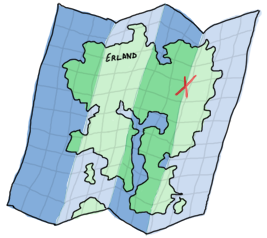
\includegraphics[width=1\linewidth]{erland.png}
\end{wrapfigure}
В начале этой главы я кратко продемонстрировал, как преобразовать две подобные функции в функцию \ops{map/2}.
Также я утверждал, что такую функцию можно использовать для любого списка, в котором мы хотим производить какое\--либо действие с каждым элементом.
Функция выглядела следующим образом:
\begin{lstlisting}[style=erlang]
map(_, []) -> [];
map(F, [H|T]) -> [F(H)|map(F,T)].
\end{lstlisting}
Однако, существует много других абстракций, подобных этой, которые можно построить из часто встречающихся рекурсивных функций.
Давайте для начала взглянем на парочку функций:
\begin{lstlisting}[style=erlang]
%% only keep even numbers
even(L) -> lists:reverse(even(L,[])).
 
even([], Acc) -> Acc;
even([H|T], Acc) when H rem 2 == 0 ->
    even(T, [H|Acc]);
even([_|T], Acc) ->
    even(T, Acc).
 
%% only keep men older than 60
old_men(L) -> lists:reverse(old_men(L,[])).
 
old_men([], Acc) -> Acc;
old_men([Person = {male, Age}|People], Acc) when Age > 60 ->
    old_men(People, [Person|Acc]);
old_men([_|People], Acc) ->
    old_men(People, Acc).
\end{lstlisting}

Первая принимает список чисел и возвращает только чётные.
Вторая проходит по списку с данными вида \{Пол, Возраст\} и возвращает лишь записи о мужчинах старше 60 лет.
В этих функциях найти общее немного сложнее, но некоторое подобие всё же есть.
Обе функции работают над списками, возвращают элементы, которые прошли некий тест (его ещё называют \emph{предикатом}), а остальные элементы отбрасывают.
Из этого обобщения мы можем извлечь всю необходимую нам информацию и преобразовать её в функцию:
\begin{lstlisting}[style=erlang]

filter(Pred, L) -> lists:reverse(filter(Pred, L,[])).
 
filter(_, [], Acc) -> Acc;
filter(Pred, [H|T], Acc) ->
    case Pred(H) of
        true  -> filter(Pred, T, [H|Acc]);
        false -> filter(Pred, T, Acc)
    end.
\end{lstlisting}

Чтобы воспользоваться функцией\--фильтром, нам необходимо лишь получить извне тестирующую функцию.
Скомпилируйте модуль \ops{\href{http://learnyousomeerlang.com/static/erlang/hhfuns.erl}{hhfuns}} и попробуйте им воспользоваться:
\begin{lstlisting}[style=erlang]
1> c(hhfuns).
{ok, hhfuns}
2> Numbers = lists:seq(1,10).
[1,2,3,4,5,6,7,8,9,10]
3> hhfuns:filter(fun(X) -> X rem 2 == 0 end, Numbers).
[2,4,6,8,10]
4> People = [{male,45},{female,67},{male,66},{female,12},{unkown,174},{male,74}].
[{male,45},{female,67},{male,66},{female,12},{unkown,174},{male,74}]
5> hhfuns:filter(fun({Gender,Age}) -> Gender == male andalso Age > 60 end, People).
[{male,66},{male,74}]
\end{lstlisting}

Эти примеры демонстрируют, что программисту, который использует функцию \ops{filter/2}, нужно лишь задать предикат и указать список, который будет фильтроваться.
О самом процессе перемещения по списку и об отбрасывании ненужных элементов думать больше не нужно.
При обобщении функционального кода происходит одна важная вещь: мы пытаемся избавиться от того, что остаётся постоянным, и позволяем программисту предоставить лишь то, что подвергается изменению.

В предыдущей главе мы применяли к спискам другой вид рекурсивных манипуляций, в котором мы последовательно рассматривали каждый элемент списка и приводили их к одному ответу.
Эта операция называется \emph{свёрткой} (fold) и может применяться для следующих функций:
\begin{lstlisting}[style=erlang]
%% find the maximum of a list
max([H|T]) -> max2(T, H).
 
max2([], Max) -> Max;
max2([H|T], Max) when H > Max -> max2(T, H);
max2([_|T], Max) -> max2(T, Max).
 
%% find the minimum of a list
min([H|T]) -> min2(T,H).
 
min2([], Min) -> Min;
min2([H|T], Min) when H < Min -> min2(T,H);
min2([_|T], Min) -> min2(T, Min).
 
%% sum of all the elements of a list
sum(L) -> sum(L,0).
 
sum([], Sum) -> Sum;
sum([H|T], Sum) -> sum(T, H+Sum).
\end{lstlisting}
\begin{wrapfigure}{r}{0.3\linewidth}
    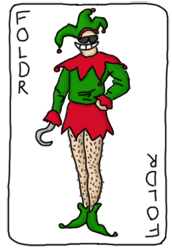
\includegraphics[width=1\linewidth]{foldr.png}
\end{wrapfigure}

Чтобы понять как себя ведёт свёртка, нам необходимо найти общее в этих действиях, а после найти различия.
Как было указано выше, мы всегда приводим список к единичному значению.
Следовательно, наша свёртка должна повторять действие, сохраняя один элемент.
Нам не нужно строить новый список.
Стражи нам не понадобятся, так как они присутствуют не всегда, а поэтому должны находиться в пользовательской функции.
В этом отношении наша функция свёртки будет, скорее всего, походить на функцию sum.

Ещё одной неприметной частью всех трёх функций, о которой мы пока не упоминали, является то, что у каждой функции должно быть начальное значение, от которого будет начинаться отсчёт.
В случае \ops{sum/2} мы используем 0, так как проводим операцию сложения, которая нейтральна относительно 0, и при вычислении \ops{X = X + 0} мы никак не повлияем на результат.
Если бы мы использовали операцию умножения \ops{X = X * 1}, то в качестве стартового значения избрали бы 1.
У функций \ops{min/1} и \ops{max/1} стартового значения по умолчанию быть не может.
Если список полностью состоит из отрицательных чисел, а мы начнём с 0, то получим неверный результат.
Поэтому нам необходимо использовать в качестве начальной точки первый элемент списка.
К сожалению, мы не можем заранее применить такие рассуждения к любой ситуации, а поэтому оставляем решение этой проблемы программисту.
Принимая во внимание все перечисленные элементы, мы можем построить следующую абстракцию:
\begin{lstlisting}[style=erlang]
fold(_, Start, []) -> Start;
fold(F, Start, [H|T]) -> fold(F, F(H,Start), T).
\end{lstlisting}
А затем исполнить:
\begin{lstlisting}[style=erlang]
6> c(hhfuns).
{ok, hhfuns}
7> [H|T] = [1,7,3,5,9,0,2,3].   
[1,7,3,5,9,0,2,3]
8> hhfuns:fold(fun(A,B) when A > B -> A; (_,B) -> B end, H, T).
9
9> hhfuns:fold(fun(A,B) when A < B -> A; (_,B) -> B end, H, T).
0
10> hhfuns:fold(fun(A,B) -> A + B end, 0, lists:seq(1,6)).
21
\end{lstlisting}

Практически любую функцию, которая сводит список значений к одному элементу, можно выразить в виде свёртки.

Забавно то, что вы можете представить аккумулятор как единичный элемент (или единичную переменную), а аккумулятор может быть списком.
Следовательно, мы можем использовать свёртку для построения списков.
Это означает, что свёртка универсальна в том смысле, что с её помощью можно реализовать практически любую другую рекурсивную функцию для списков, даже отображение и фильтр:
\begin{lstlisting}[style=erlang]
reverse(L) ->
    fold(fun(X,Acc) -> [X|Acc] end, [], L).
 
map2(F,L) ->
    reverse(fold(fun(X,Acc) -> [F(X)|Acc] end, [], L)).
 
filter2(Pred, L) ->
    F = fun(X,Acc) ->
        case Pred(X) of
            true  -> [X|Acc];
            false -> Acc
        end
    end,
    reverse(fold(F, [], L)).
\end{lstlisting}

И эти функции будут работать так же как и те, что мы написали ранее.
Ну как, мощные абстракции или нет?

Отображение, фильтры и свёртки \--- это лишь часть функций для списков, которые предоставляются стандартной библиотекой Erlang (см. \ops{\href{http://erldocs.com/R15B/stdlib/lists.html\#map/2}{lists:map/2}}, \ops{\href{http://erldocs.com/R15B/stdlib/lists.html\#filter/2}{lists:filter/2}}, \ops{\href{http://erldocs.com/R15B/stdlib/lists.html\#foldl/3}{lists:foldl/3}} и \ops{\href{http://erldocs.com/R15B/stdlib/lists.html\#foldr/3}{lists:foldr/3}}.
Стоит отметить также функции \ops{\href{http://erldocs.com/R15B/stdlib/lists.html\#all/2}{all/2}} и \ops{\href{http://erldocs.com/R15B/stdlib/lists.html\#any/2}{any/2}}, которые принимают предикат и проверяют, что для каждого элемента предикат возвращает true, или что хотя бы для одного из них предикат возвращает true, соответственно.
Ещё есть функция \ops{\href{http://erldocs.com/R15B/stdlib/lists.html\#dropwhile/2}{dropwhile/2}}, которая игнорирует элементы списка до тех пор, пока не находит один, удовлетворяющий предикату, и противоположная функция \ops{\href{http://erldocs.com/R15B/stdlib/lists.html\#takewhile/2}{takewhile/2}}, которая будет возвращать элементы до тех пор, пока не встретит такой, для которого предикат не возвращает true.
Две предыдущие функции объединяет \ops{\href{http://erldocs.com/R15B/stdlib/lists.html\#partition/2}{partition/2}}.
Эта функция принимает один список, а возвращает два.
Первый содержит термы, которые удовлетворяют предикату, а второй \--- остальные элементы. Кроме того, для обработки списков часто используются такие функции как \ops{\href{http://erldocs.com/R15B/stdlib/lists.html\#flatten/1}{flatten/1}}, \ops{\href{http://erldocs.com/R15B/stdlib/lists.html\#flatlength/1}{flatlength/1}}, \ops{\href{http://erldocs.com/R15B/stdlib/lists.html\#flatmap/2}{flatmap/2}}, \ops{\href{http://erldocs.com/R15B/stdlib/lists.html\#merge/1}{merge/1}}, \ops{\href{http://erldocs.com/R15B/stdlib/lists.html\#nth/2}{nth/2}}, \ops{\href{http://erldocs.com/R15B/stdlib/lists.html\#nthtail/2}{nthtail/2}}, \ops{\href{http://erldocs.com/R15B/stdlib/lists.html\#split/2}{split/2}} и другие.

Также там можно найти другие функции, такие как zip\--функция (которую мы рассматривали в предыдущей главе), unzip\--функция, комбинации отображений и свёрток и т.д.
Рекомендую вам прочитать \href{http://erldocs.com/R15B/stdlib/lists.html}{описание списков}.
В этом документе вы найдёте примеры использования списковых функций.
Применяя те концепции, которые были заключены умными людьми в этих абстракциях, у вас редко будет появляться необходимость в самостоятельном создании рекурсивных функций.

\chapter{Ошибки и исключения}
\label{errors-and-exceptions}
\section{Придержи коней!}
\begin{wrapfigure}{r}{0.4\linewidth}
    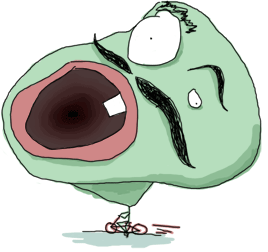
\includegraphics[width=1\linewidth]{cyclist.png}
\end{wrapfigure}
Для этой главы невозможно подобрать подходящее место в книге.
К этому моменту вы изучили уже достаточно, чтобы начать натыкаться на ошибки, но ещё недостаточно, чтобы знать, как их контролировать.
По правде говоря, в этой главе мы не сможем рассмотреть все механизмы управления ошибками.
Отчасти это невозможно потому, что в Erlang существуют две главные парадигмы: функциональная и параллельная (concurrent).
О функциональной я рассказываю с самого начала книги: ссылочная прозрачность (чистота, referntial transparency), рекурсия, функции высшего порядка и т.д.
Но именно параллельная часть прославила Erlang: акторы, тысячи и тысячи параллельных (concurrent) процессов, деревья контроля и т.д.

Я считаю, что прежде чем переходить к параллельной части, совершенно необходимо изучить функциональную.
Поэтому я затрону лишь функциональное подмножество языка.
Чтобы управлять ошибками, нам нужно сначала их понять.\\
\colorbox{lgray}
{
\begin{minipage}{1.0\linewidth}
    \textbf{Замечание:} хоть Erlang и позволяет обращаться с ошибками в функциональном коде сразу несколькими способами, но чаще всего вы будете слышать, что делать ничего не нужно, а нужно позволить процессу упасть.
    Я уже намекал на это во \ref{introduction}~введении.
    Механизмы, которые позволяют вам программировать в таком стиле, находятся в параллельной части языка.
\end{minipage}
}
\section{Компиляция ошибок}
Ошибки подразделяются на множество видов: ошибки времени компиляции, логические ошибки, ошибки времени исполнения и сгенерированные ошибки.
В этом разделе я сконцентрирую внимание на ошибках времени компиляции, а о других расскажу чуть позже.

Ошибки времени компиляции чаще всего являются синтаксическими ошибками: нужно проверить наименование функций, языковые токены (скобки, квадратные скобки, точки, запятые), арность ваших функций и т.д.
Вот список некоторых часто встречающихся проблем времени компиляции и потенциальные способы их разрешения:

\blankline
\begin{minipage}{\textwidth}
\textbf{module.beam: Module name 'madule' does not match file name 'module'}\\
Имя модуля, которое вы указали в атрибуте \ops{-module} не совпадает с именем файла.
\end{minipage}

\blankline
\begin{minipage}{\textwidth}
\textbf{./module.erl:2: Warning: function some\_function/0 is unused}\\ 
Вы не проэкспортировали функцию, либо в месте её использования указано неверное имя или арность.
Возможно также, что вы записали функцию, которая больше нигде не вызывается.
Проверьте ваш код!
\end{minipage}

\blankline
\begin{minipage}{\textwidth}
\textbf{./module.erl:2: function some\_function/1 undefined}\\ 
Функция не существует.
Вы ввели неверное имя или указали неверную арность либо в атрибуте \ops{-export}, либо во время определения функции.
Это сообщение также можно увидеть, когда данная фунция не может быть скомпилирована.
Обычно такое случается из\--за какой\--либо синтаксической ошибки, например если вы забыли поставить точку в конце функции.
\end{minipage}

\blankline
\begin{minipage}{\textwidth}
\textbf{./module.erl:5: syntax error before: 'SomeCharacterOrWord'}\\ 
Эта ошибка может быть вызвана множеством причин, а именно: незакрытыми скобками, неверным завершением кортежа или выражения (когда вы, к примеру, закрыли заключительную ветку \ops{case} при помощи запятой).
Среди других причин можно выделить использование зарезервированного атома в вашем коде, либо юникодного символа, который был искажён при перекодировке (я видел и такое!)
\end{minipage}

\blankline
\begin{minipage}{\textwidth}
\textbf{./module.erl:5: syntax error before: }\\ 
Да уж, смысл сообщения не вполне очевиден.
Эта ошибка выдаётся, когда неверно завершена одна из строк.
Она является частным случаем предыдущей ошибки.
Просто будьте внимательны.
\end{minipage}

\blankline
\begin{minipage}{\textwidth}
\textbf{./module.erl:5: Warning: this expression will fail with a 'badarith' exception}\\
Всё в Erlang вертится вокруг динамической типизации, но не забывайте, что типизация также и сильная.
В этом примере у компилятора хватило сообразительности, чтобы определить, что в одном из арифметических выражений кроется ошибка (например, \ops{llama + 5}).
Впрочем, более сложные ошибки типов пройдут незамеченными.
\end{minipage}

\blankline
\begin{minipage}{\textwidth}
    \textbf{./module.erl:5: Warning: variable 'Var' is unused}\\
    Вы объявили переменную и нигде её не использовали.
    Это может оказаться ошибкой, так что перепроверьте ваш код.
    Если вы это сделали намеренно, то наверняка лучше поменять имя переменной на \ops{\strut{\_}} или поместить перед именем переменной знак подчёркивания (что\--то вроде \emph{\_Var}).
    Так следует поступить, когда вы считаете, что наличие имени улучшит читабельность кода.
\end{minipage}

\blankline
\begin{minipage}{\textwidth}
    \textbf{./module.erl:5: Warning: a term is constructed, but never used}\\
    Вы создали в одной из ваших функций кортеж, список, или анонимную функцию, которую впоследствии не связали с переменной и не использовали в качестве возвращаемого значения.
    Это предупреждение сообщает, что вы создаёте что\--либо впустую или совершили какую\--либо ошибку.
\end{minipage}

\blankline
\begin{minipage}{\textwidth}
    \textbf{./module.erl:5: head mismatch}\\
    Возможно, у вашей функции несколько заголовков с различной арностью.
    Не забывайте, что изменяя арность можно создавать разные функции с одинаковыми именами.
    В объявлении одной функции нельзя чередовать заголовки с разной арностью.
    Эту ошибку также можно встретить, когда между заголовками одной функции вставляют определение другой.
\end{minipage}

\blankline
\begin{minipage}{\textwidth}
    \textbf{./module.erl:5: Warning: this clause cannot match because a previous clause at line 4 always matches}\\
    У функции, определённой в модуле, после универсального условия указано конкретное.
    Поэтому компилятор предупреждает, что до более конкретного условия исполнение не дойдёт.
\end{minipage}

\blankline
\begin{minipage}{\textwidth}
    \textbf{./module.erl:9: variable 'A' unsafe in 'case' (line 5)}\\
    Переменная, определённая в одной из веток выражения \ops{case\ldots of}, используется вне этого выражения.
    Такое поведение считается небезопасным.
    Если вам понадобились такие переменные, их лучше объявлять при помощи конструкции \ops{MyVar = case \ldots of}\ldots
\end{minipage}

Этот перечень покрывает большинство ошибок компиляции, с которыми вы можете столкнуться на текущий момент. Их не так уж и много, поэтому зачастую сложнее всего найти ошибку, которая вызвала каскад ошибок, найденных в других функциях.
Ошибки, которые выдаёт компилятор, лучше всего исправлять в том порядке, в котором они указаны в списке, чтобы не начать исправлять ошибки, которые могут ими и не являться.
Иногда можно наткнуться и на другие сообщения, которые в список не попали.
Если вы с таким столкнулись, то напишите мне по email, и я как можно быстрее добавлю его в список вместе с комментариями.
\section{Нет, это у ТЕБЯ неправильная логика!}
\label{no-your-logic-is-wrong}
\begin{wrapfigure}{r}{0.35\linewidth}
    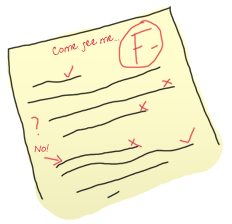
\includegraphics[width=1\linewidth]{exam.png}
\end{wrapfigure}
Логические ошибки искать и отлаживать сложнее всего. Чаще всего эти ошибки делает сам программист: ветвления и условия (например if\--ы и case\--ы), в которых не учитываются все случаи, употребление умножения вместо деления и т.д.
Такие ошибки не приводят к аварийному завершению программы, но из\--за них программа может просто выдать неверные данные или работать незапланированным образом.

С такими ошибками вам придётся справляться самостоятельно, но в Erlang есть много средств, которые придут вам на помощь.
В их числе тестовые фреймворки, TypEr и Dialyzer (которые описывались в \ref{for-type-junkies}~главе о типах), \ref{debugger-chapter}~отладчик, \ref{dbg}~модуль трассировки и т.д.
Лучшая защита от таких ошибок \--- это тестирование.
В карьере любого программиста, к сожалению, таких ошибок хватит на пару дюжин книг, поэтому я не буду тратить на них много времени.
Легче сконцентрироваться на тех ошибках, которые приводят к аварийному завершению, так как момент их появления ясен, и они не всплывут на поверхность через 50 уровней вложенности.
Это соображение, как раз, и служит источником мантры: <<пусть процесс падает>>, о которой я уже несколько раз упоминал.
\section{Ошибки времени исполнения}
\label{run-time-errors}
Ошибки времени исполнения (run\--time errors) весьма разрушительно влияют на ваш код. Они приводят к аварийной ситуации.
Хотя в Erlang и существуют методы их контроля, но никогда не бывает лишним умение эти ошибки различать.
Поэтому я составил небольшой список таких ошибок с объяснением и примерами кода, который может их вызвать.

\textbf{function\_clause}
\begin{lstlisting}[style=erlang]
1> lists:sort([3,2,1]).
[1,2,3]
2> lists:sort(fffffff).
** exception error: no function clause matching lists:sort(fffffff)
\end{lstlisting}

Все охранные выражения завершились неудачей, либо для функции не сработал ни один из шаблонов для сопоставления с образцом.
\blankline

\textbf{case\_clause}
\begin{lstlisting}[style=erlang]
3> case "Unexpected Value" of
3>    expected_value -> ok;
3>    other_expected_value -> 'also ok'
3> end.
** exception error: no case clause matching "Unexpected Value"
\end{lstlisting}

Похоже, что кто\--то забыл указать шаблон в выражении \ops{case}, передал неподходящие данные, или забыл задать вариант для выбора по умолчанию.
\blankline

\textbf{if\_clause}
\begin{lstlisting}[style=erlang]
4> if 2 > 4 -> ok;
4>    0 > 1 -> ok
4> end.
** exception error: no true branch found when evaluating an if expression
\end{lstlisting}

Это сообщение очень похоже на ошибки \ops{case\_clause}. Не получается найти ветку, которая принимает значение \ops{true}.
Скорее всего, необходимо убедиться, что обрабатываются все возможные случаи, либо добавить вариант \ops{true} для выбора по умолчанию.
\blankline

\textbf{badmatch}
\begin{lstlisting}[style=erlang]
5> [X,Y] = {4,5}.
** exception error: no match of right hand side value {4,5}
\end{lstlisting}

Такие ошибки возникают в случае, когда не удаётся провести операцию сопоставления с образцом.
Скорее всего, вы пытаетесь провести невозможное сопоставление, пытаетесь связать переменную со значением во второй раз, или по обе стороны оператора \ops{\strut=} находятся неравные значения (что, в общем\--то и приводит к тому, что операция связывания завершается неудачей!).
Заметьте, что иногда эта ошибка возникает, потому что по мнению программиста переменная вида \emph{\_MyVar} означает то же самое, что и \ops{\strut\_}.
Переменные, имя которых начинается со знака подчёркивания \--- это обычные переменные.
Единственное их отличие в том, что компилятор не генерирует предупреждение, если эти переменные не используются после объявления.
Их можно связать со значением лишь один раз.
\blankline

\textbf{badarg}
\begin{lstlisting}[style=erlang]
6> erlang:binary_to_list("heh, already a list").
** exception error: bad argument
    in function  binary_to_list/1
        called as binary_to_list("heh, already a list")
\end{lstlisting}

Эта ошибка похожа на \ops{function\_clause} тем, что она сообщает о вызове функции с некорректными аргументами.
Главное отличие в том, что ошибка генерируется программистом, который проверяет аргументы в теле функции, а не в охранных выражениях (стражах).
Чуть позже в этой главе я покажу как генерировать такие ошибки.
\blankline

\textbf{undef}
\begin{lstlisting}[style=erlang]
7> lists:random([1,2,3]).
** exception error: undefined function lists:random/1
\end{lstlisting}
Ошибка генерируется, когда вы пытаетесь вызвать несуществующую функцию.
Убедитесь, что функция экспортируется из модуля с правильной арностью (если вы вызываете её вне модуля), и перепроверьте правильность написания имени функции и модуля.
Ещё одной причиной получения этого сообщения может служить то, что модуль находится вне пути поиска Erlang.
По умолчанию поиск происходит в текущей директории. Добавлять пути можно при помощи функции \ops{code:add\_patha/1} или \ops{code:add\_pathz/1}.
Если ничего из перечисленного не помогает, то сперва убедитесь, что модуль скомпилирован!
\blankline

\textbf{badarith}
\begin{lstlisting}[style=erlang]
8> 5 + llama.
** exception error: bad argument in an arithmetic expression
    in operator  +/2
        called as 5 + llama
\end{lstlisting}

Это сообщение появляется, когда вы пытаетесь выполнить несуществующее арифметическое действие.
Например, делите на ноль или пытаетесь выполнять арифметические операции между атомами и числами.
\blankline

\textbf{badfun}
\begin{lstlisting}[style=erlang]
9> hhfuns:add(one,two).
** exception error: bad function one
in function  hhfuns:add/2
\end{lstlisting}
Чаще всего причиной возникновения этой ошибки становится попытка использовать переменные в качестве функций, но при этом переменные функций не содержат.
В приведённом выше примере я использую функцию \ops{hhfuns} из предыдущей главы \ref{higher-order-functions}~и при этом передаю в качестве параметров\--функций пару атомов.
Такой код не сработает, и будет выброшена ошибка \ops{badfun}.
\blankline

\textbf{badarity}
\begin{lstlisting}[style=erlang]
10> F = fun(_) -> ok end.
#Fun<erl_eval.6.13229925>
11> F(a,b).
** exception error: interpreted function with arity 1 called with two arguments
\end{lstlisting}
Ошибка \ops{badarity} \--- это частный случай ошибки \ops{badfun}. 
Она происходит, когда вы используете функции высшего порядка, которым передаёте больше (или меньше) аргументов, чем они требуют.
\blankline

\textbf{system\_limit}

Есть много причин, по которым может быть сгенерирована ошибка \ops{system\_limit}: слишком много процессов (мы до них ещё доберёмся), слишком длинные атомы, у функции слишком много аргументов, количество атомов слишком велико, слишком много подсоединённых узлов и т.д.
Полный список можно прочитать в \href{http://www.erlang.org/doc/efficiency_guide/advanced.html#id2265856}{Erlang Efficiency Guide} в разделе о системных ограничениях (system limits).
Примите к сведению, что некоторые из этих ошибок настолько серьёзны, что могут привести к аварии всей виртуальной машины.

\section{Вызываем исключения}
\label{raising-exceptions}
Чтобы следить за исполнением кода и защититься от логических ошибок, иногда полезно провоцировать аварийную остановку во время исполнения кода, чтобы как можно раньше выявить возможные проблемы.
В Erlang существуют три вида исключений: \emph{ошибки (errors)}, \emph{броски (throws)} и \emph{завершения (exits)}. Все они используются в разных случаях (ну или почти в разных):

\begin{wrapfigure}{r}{0.35\linewidth}
    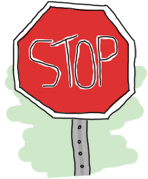
\includegraphics[width=1\linewidth]{stop.png}
\end{wrapfigure}

\subsection{Ошибки}
\label{errors}
Вызов \ops{erlang:error(Reason)} завершит исполнение в текущем процесе и, после того как исключение будет поймано, предоставит трассировку стека и список аргументов для последних вызовов функций.
Это тот самый вид исключений, который вызывает ошибки времени исполнения, о которых я упоминал выше.

При помощи ошибок (errors) можно останавливать исполнение кода, в случае когда вызываемый код определённо не сможет справиться с той ситуацией, в которую он попадёт после вызова.
Если вам была возвращена ошибка \ops{if\_clause}, что вы сделаете?
Измените код, перекомпилируете его \--- вот и всё что вы можете (ну, ещё можно отобразить красивое сообщение об ошибке).
Как пример того, где не следует использовать ошибки, можно упомянуть наш модуль для работы с деревьями из главы о рекурсии \ref{recursion}.
Поиск по дереву, реализованный в модуле, не сможет найти ключ, которого в дереве нет.
В такой ситуации можно было бы ожидать, что с неизвестным результатом разберётся сам пользователь. 
Он сможет использовать значение по умолчанию, удалить дерево.
А может быть он просто проверял, есть ли в дереве какой\--либо ключ, чтобы добавить новый и т.д.
Здесь вместо вызова ошибки лучше было бы возвратить кортеж \ops{\{ok, Value\}}, или атом \ops{undefined}.

Но область применения ошибок не ограничивается лишь этими примерами.
Можно также определить собственный вид ошибок:
\begin{lstlisting}[style=erlang]
1> erlang:error(badarith).
** exception error: bad argument in an arithmetic expression
2> erlang:error(custom_error).
** exception error: custom_error
\end{lstlisting}

В этом примере оболочка Erlang не распознала \ops{custom\_error} и не вывела сообщение вида ``bad argument in \ldots'', но тем не менее эту ошибку можно использовать и обрабатывать так же как обычно (скоро мы увидим как это делать).

\subsection{Завершения}
\label{exits}
Существует два вида завершений: 'внутренние' (internal) и 'внешние' (external).
Внутренние завершения выполняются посредством вызова функции \ops{exit/1} и приводят к остановке текущего процесса.
Внешние завершения выполняются функцией \ops{exit/2} и имеют отношение к множеству процессов, принадлежащих к параллельной (concurrent) части Erlang; поэтому здесь мы сосредоточимся на внутренних завершениях, а к внешним обратимся чуть позже.

Внутренние завершения очень похожи на ошибки (errors).
На самом деле, раньше они были одним целым в составе функции \ops{exit/1}.
Использовали их в приблизительно тех же случаях.
Так как же определить, что использовать в конкретной ситуации?
Принцип выбора неочевиден.
Чтобы понять, когда нужно использовать ту или иную конструкцию, ничего не остаётся кроме как начать постепенно знакомиться с концепциями акторов и процессов.

Во введении я сравнивал процессы с людьми, которые общаются посредством почты. К этой аналогии, в общем\--то, добавить нечего, поэтому перейду к диаграммам и кружкам.
\begin{figure}[h!]
    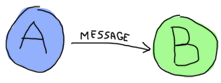
\includegraphics[width=0.4\textwidth]{a-b-msg.png}
\end{figure}

Эти процессы могут посылать друг другу сообщения.
Процесс также может ожидать прихода каких\--либо сообщений.
Можно выбирать, какие сообщения нужно ждать, какие отклонять, а какие игнорировать, через какой период времени прекращать ожидание и т.д.
\begin{figure}[h!]
    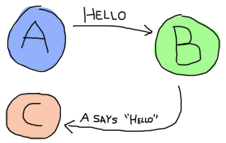
\includegraphics[width=0.4\textwidth]{a-b-c-hello.png}
\end{figure}

Эти основные концепции позволяют создателям Erlang использовать особенный вид сообщений, при помощи которых между процессами передаются исключения.
Они работают как своего рода <<последний вздох>> процесса; их посылают прямо перед тем, как процесс умирает и его код перестаёт выполняться.
Другие процессы, которые ожидали этот вид сообщений, смогут узнать об этом событии и распорядиться этим знанием как угодно.
Сделать запись в журнале, перезапустить умерший процесс и т.д.
\begin{figure}[h!]
    
\includegraphics[width=0.4\textwidth]{a-b-dead.png}
\end{figure}

Ну а теперь, когда мы имеем представление об этой концепции, нам будет проще понять разницу между \ops{erlang:error/1} и \ops{exit/1}.
Обе функции можно использовать очень похожим способом, но настоящая разница заключается в нашем намерении.
После получения такой ошибки можно решить, была ли это <<просто>> ошибка или ошибка из\--за которой стоит убить текущий процесс.
Это соображение подкрепляется тем, что функция \ops{erlang:error/1} возвращает трассировку стека, а \ops{exit/1} этого не делает.
Если бы ваша трассировка стека была достаточно велика, или у текущей функции было бы много аргументов, то отсылка сообщений о завершении каждому процессу, который ожидает такое сообщение, означало бы, что эти данные необходимо копировать. В некоторых случаях это может оказаться непрактичным.
\subsection{Броски}
\label{throws}
Броски \--- это класс исключений, используемых в случаях, которые должен обрабатывать сам программист..
По сравнению с завершениями  или ошибками, броски не имеют коннотации <<роняй процесс!>>.
Они больше относятся к управлению логикой программы.
Когда вы используете броски и ожидаете, что их будет обрабатывать программист, не лишним будет задокументировать этот факт в модуле, который их содержит.

Синтаксис бросков следующий:
\begin{lstlisting}[style=erlang]
1> throw(permission_denied).
** exception throw: permission_denied
\end{lstlisting}
\ops{permission\_denied} можно заменить чем угодно (даже сообщением \ops{'всё в порядке'}, но оно вряд ли окажется полезным для кого\--либо, а вот друзей с таким кодом вы точно не приобретёте).

Броски также можно использовать для нелокального возврата из глубокой рекурсии.
Можно привести модуль \ops{\href{http://erldocs.com/R15B/ssl/ssl.html}{ssl}} в качестве примера.
Он использует функцию \ops{throw/1} для того, чтобы протолкнуть кортежи \ops{\{error, Reason\}} назад вызывающей функции.
В свою очередь, она просто возвращает кортеж пользователю.
Благодаря этому разработчик может писать код, который рассматривает только благополучные варианты развития событий, а все исключения обрабатывает лишь в одной вышестоящей функции.

Ещё одним примером может послужить модуль для работы с массивами, в котором есть функция поиска.
В случае, если нужный элемент не был найден, эта функция возвращает значение по умолчанию, предоставленное пользователем.
Когда элемент не удаётся найти, в исключении бросается значение \ops{default}, которое обрабатывает вышестоящая функция и заменяет на пользовательское значение по умолчанию.
Это избавляет программиста модуля от необходимости передавать значение по умолчанию в каждую функцию алгоритма поиска и позволяет сконцентрироваться лишь на благополучных исходах.

Чтобы облегчить отладку кода, старайтесь использовать броски для нелокальных возвратов только в одном модуле.
К тому же, это позволит изменять внутреннее устройство модуля без необходимости менять его интерфейс.

\chapter{Решаем задачи в функциональном стиле}
\label{functionally-solving-problems}
\colorbox{lgray}
{
\begin{minipage}{1.0\linewidth}
    Похоже, что мы уже выпили достаточно эрлангового сока, чтобы создать что\--нибудь полезное.
    В этой главе не будет нового материала.
    Я просто покажу как применять элементы увиденного ранее.
    Задачи были взяты из книги Miran\--а \href{http://learnyouahaskell.com/functionally-solving-problems}{Learn You a Haskell}.
    Для всех примеров я использовал аналогичный способ решения, чтобы любопытный читатель смог сравнивать код на Erlang и Haskell как ему заблагорассудится.
    Проведя такое сравнение, вы, наверняка, придёте к заключению, что для двух языков с очень разными синтаксисами, решения очень похожи друг на друга.
    Это сходство обусловлено тем, что изученные концепции функционального программирования можно сравнительно легко переносить на другие функциональные языки.
\end{minipage}
}
\section{Калькулятор в обратной польской записи}
\label{reverse-polish-notation-calculator}
Большинство людей обучены записи арифметических выражений, согласно которой оператор помещают между числами (\ops{(2 + 2) / 5}).
Так вводятся математические выражения в большинстве калькуляторов, и, скорее всего,  такую запись вас обучили использовать при счёте на школьных уроках. 
У этой записи есть недостаток: вам необходимо знать порядок вычисления операторов.
Умножение и деление считается более важным (имеет более высокий приоритет), чем сложение и вычитание.

Существует ещё один способ записи, который называется \emph{префиксной записью} или \emph{польской записью}, в которой оператор записывается перед операндами.
В этой записи выражение \ops{(2 + 2) / 5} примет вид \ops{(/ (+ 2 2) 5)}.
Если мы решим, что \ops{+\strut}  и \ops{/\strut} должны всегда принимать два аргумента, то \ops{(/ (+ 2 2) 5)} можно просто записать как \ops{/ + 2 2 5}.

Однако, мы сосредоточимся на \emph{обратной польской записи} (или просто ОПЗ), которая противоположна префиксной записи: в ней оператор следует за операндами.
Тот же самый пример, приведённый выше, в ОПЗ будет записан как \ops{2 2 + 5 /}.
Можно привести и другие примеры: \ops{9 * 5 + 7} и \ops{10 * 2 * (3 + 5) / 2} транслируются соответственно в \ops{9 5 * 7} и \ops{10 2 * 3 4 + * 2 /}.
Эта запись очень широко использовалась в ранних моделях калькуляторов, так как экономно использует память.
А некоторые люди до сих пор таскают с собой калькуляторы с ОПЗ.
Именно такой калькулятор мы и напишем.

Для начала, неплохо было бы понимать, как читаются выражения ОПЗ.
Первый способ: по одному находим операторы и, учитывая арность, группируем их с операндами.
\begin{align*}
    &10\;4\;3+2 * -\\
    &10\;(4\;3\; +)\;2 * -\\
    &10\; ((4\; 3\; +)\; 2\; *) -\\ 
    &(10\; ((4\; 3\; +)\; 2\; *) -)\\
    &(10\; (7\; 2\; *) -)\\
    &(10\; 14\; -)\\
    &-4\\
\end{align*}

Однако, в компьютере или калькуляторе намного проще создать \emph{стек} всех операндов в порядке их расположения.
Возьмём математическое выражение \ops{10 4 3 + 2 * -}.
Первый операнд 10.
Мы добавляем его в стек.
Затем идёт 4.
Его мы тоже кладём на вершину стека.
Третьим идёт число 3.
Мы помещаем в стек и его.
Теперь стек принял следующий вид:
\begin{figure}[h!]
    \centering
    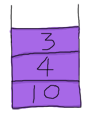
\includegraphics[width=0.12\textwidth]{stack1.png}
\end{figure}

Следующий символ это \ops{+\strut}.
Он представляет собой функцию арности 2.
Чтобы ею воспользоваться, нам необходимо передать ей два операнда, которые мы извлечём из стека:
\begin{figure}[h!]
    \centering
    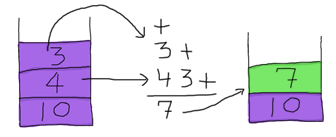
\includegraphics[width=0.4\textwidth]{stack2.png}
\end{figure}

Полученную цифру 7 мы загоняем в верхушку стека (фу, мы же не хотим, чтобы эти грязные числа шатались повсюду!)
Теперь стек содержит [7, 10], и от первоначального выражения осталось лишь \ops{2 * -}.
Мы берём 2 и помещаем его в вершину стека.
Затем мы видим операцию \ops{*\strut}, которой для работы необходимо передать два операнда.
И снова мы извлекаем их из стека:
\begin{figure}[h!]
    \centering
    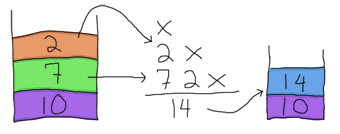
\includegraphics[width=0.4\textwidth]{stack3.png}
\end{figure}

И помещаем 14 в вершину стека.
Остаётся лишь \ops{-\strut}, которому необходимо передать два операнда.
Невероятная удача!
В стеке как раз осталось два операнда.
Пустим их в дело!
\begin{figure}[h!]
    \centering
    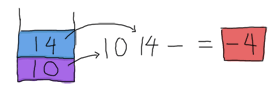
\includegraphics[width=0.4\textwidth]{stack4.png}
\end{figure}

Ну вот мы и получили результат.
Этот стек\--ориентированный подход сравнительно надёжен.
Тот факт, что для начала вычислений требуется разбирать мало данных, объясняет почему этот способ годится даже для старых калькуляторов.
ОПЗ стоит использовать и по другим причинам, но их обсуждение выходит за рамки этого руководства..
Заинтересовавшимся лучше обратиться к \href{http://en.wikipedia.org/wiki/Reverse_Polish_notation}{статье на Wikipedia}.

Как только мы справились со сложными моментами, записать решение на Erlang становится достаточно просто.
Оказывается, самое сложное \--- определить шаги для получения конечного результата.
А это мы только что проделали.
Неплохо.
Откройте файл \emph{\href{http://learnyousomeerlang.com/static/erlang/calc.erl}{calc.erl}}.

Для начала озаботимся представлением математических выражений.
Чтобы упростить задачу мы, наверное, представим их в виде строки: \ops{''10 4 3 + 2 * -''}.
В этой строке между термами есть пробелы, которые не оговорены в нашем решении, но для работы простого лексического анализатора они необходимы.
После обработки входящей строки анализатором, мы ожидаем получить список термов вида \ops{[''10'',''4'',''3'',''+'',''2'',''*'',''-'']}.
Оказывается, функция \ops{\href{http://erldocs.com/R15B/stdlib/string.html\#tokens/2}{string:tokens/2}} делает именно то, что нам нужно:
\begin{lstlisting}[style=erlang]
1> string:tokens("10 4 3 + 2 * -", " ").
["10","4","3","+","2","*","-"]
\end{lstlisting}

Такое представление выражения нам подойдёт.
Следующим шагом мы должны определить стек.
Как мы это сделаем?
Возможно, вы заметили, что поведение списков в Erlang очень похоже на стек.
Оператор (\ops{|}) в шаблоне \ops{[Head|Tail]} ведёт себя так же как и операция добавления \emph{Head} в вершину стека (которой в данном случае является \emph{Tail}).
Список вполне сгодится на роль стека.

Чтобы прочитать выражение, нам необходимо просто повторить те же действия, которые мы выполняли при решении задачи вручную.
Последовательно считываем каждое значение в выражении.
Если мы прочитали число \--- кладём его на стек.
Если функцию \--- извлекаем все необходимые ей значения из стека, а результат вычисления возвращаем обратно в стек.
Если обобщить задачу, то нам нужно один раз пройти в цикле по всему выражению и по ходу движения накапливать результаты.
С этим прекрасно справится свёртка (fold)!

Теперь мы должны выяснить, как будет выглядеть функция, которую \ops{\href{http://erldocs.com/R15B/stdlib/lists.html\#foldl/3}{lists:foldl/3}} будет применять к каждому оператору и операнду в нашем выражении.
Функция будет запускаться в свёртке, следовательно она должна принимать два аргумента: первый будет содержать элемент выражения, который будет обрабатывать функция, а вторым будет передаваться стек.

Начнём редактировать наш код в файле \ops{\href{http://learnyousomeerlang.com/static/erlang/calc.erl}{calc.erl}}.
Напишем функцию, в которой будет происходить итерация, а также удаление пробелов из выражения:
\begin{lstlisting}[style=erlang]
-module(calc).
-export([rpn/1]).
 
rpn(L) when is_list(L) ->
    [Res] = lists:foldl(fun rpn/2, [], string:tokens(L, " ")),
    Res.
\end{lstlisting}

Следующим шагом реализуем функцию \ops{rpn/2}.
Обратите внимание: каждый оператор и операнд из выражения в конце концов попадает на вершину стека, а поэтому и конечный результат вычислений также окажется в стеке.
Мы извлечём последнее значение из стека и возвратим его пользователю.
Именно поэтому в сопоставлении с образцом мы используем шаблон \ops{[Res]} и возвращаем \emph{Res}.

Хорошо, а теперь более сложный момент.
Наша функция \ops{rpn/2} должна обрабатывать стек для всех переданных ей значений.
Заголовок функции, скорее всего, будет выглядеть как \ops{rpn(Op,Stack)}, а возвращаемое значение примет вид \ops{[NewVal|Stack]}.
Для обычных чисел будет выполняться операция:
\begin{lstlisting}[style=erlang]
rpn(X, Stack) -> [read(X)|Stack].
\end{lstlisting}

Функция \ops{read/1} конвертирует строку в целое число или число с плавающей запятой.
К сожалению, в Erlang нет встроенной функции, которая делает и то и другое, поэтому мы создадим её сами:
\begin{lstlisting}[style=erlang]
read(N) ->
    case string:to_float(N) of
        {error,no_float} -> list_to_integer(N);
        {F,_} -> F
    end.
\end{lstlisting}

Где \ops{\href{http://erldocs.com/R15B/stdlib/string.html\#to\_float/1}{string:to\_float/1}} производит конвертацию строк вида ''13.37'' в их числовой эквивалент.
Если значение числа с плавающей запятой определить не удаётся, функция возвращает \ops{\{error,no\_float\}}.
После чего мы должны вызвать функцию \ops{list\_to\_integer/1}.

А теперь снова вернёмся к \ops{rpn/2}.
Все найденные числа мы отправляем в стек.
Но так как наше сопоставление с образцом захватывает любые значения (см. \ref{pattern-matching}), то кроме чисел в стек также будут попадать и операторы.
Чтобы этого избежать, мы добавим для всех арифметических действий свои специальные заголовки с образцами для сопоставления, которые будут предварять более общий заголовок.
Начнём со сложения:
\begin{lstlisting}[style=erlang]
rpn("+", [N1,N2|S]) -> [N2+N1|S];
rpn(X, Stack) -> [read(X)|Stack].
\end{lstlisting}

Очевидно, что каждый раз когда нам попадается строка \ops{''+''}, мы извлекаем из стека два числа \emph{(N1,N2)}, складываем их и возвращаем результат в стек.
Именно такие действия мы выполняли, когда решали задачу вручную.
Запустив программу, мы сможем убедиться в её работоспособности:
\begin{lstlisting}[style=erlang]
1> c(calc).
{ok,calc}
2> calc:rpn("3 5 +").
8
3> calc:rpn("7 3 + 5 +").
15
\end{lstlisting}

Всё остальное \--- тривиально.
Нужно  лишь добавить такие же строки для всех оставшихся  операторов:
\begin{lstlisting}[style=erlang]
rpn("+", [N1,N2|S]) -> [N2+N1|S];
rpn("-", [N1,N2|S]) -> [N2-N1|S];
rpn("*", [N1,N2|S]) -> [N2*N1|S];
rpn("/", [N1,N2|S]) -> [N2/N1|S];
rpn("^", [N1,N2|S]) -> [math:pow(N2,N1)|S];
rpn("ln", [N|S])    -> [math:log(N)|S];
rpn("log10", [N|S]) -> [math:log10(N)|S];
rpn(X, Stack) -> [read(X)|Stack].
\end{lstlisting}

Обратите внимание, что функции, которые принимают лишь один аргумент (например функция логарифмирования), должны извлекать из стека один элемент.
Пусть читатель в качестве упражнения добавит функции 'sum' или 'prod', которые, соответственно, возвращают сумму и произведение всех считанных элементов.
Если у вас возникнут затруднения, обратитесь к моей реализации этих функций в \ops{\href{http://learnyousomeerlang.com/static/erlang/calc.erl}{calc.erl}}.

Мы напишем несколько простых юнит\--тестов, чтобы убедиться, что всё работает как положено.
Оператор \ops{=\strut} в Erlang можно использовать как функцию \emph{утверждения (assertion)}.
Если после проверки утверждения обнаружены значения, которые ему не соответствуют \--- должен происходить сбой.
Это как раз то, что нам нужно.
Конечно, в Erlang есть и более совершенные тестовые фреймворки, например \href{http://erlang.org/doc/apps/common_test/write_test_chapter.html}{Common Test} и \href{http://erlang.org/doc/apps/eunit/chapter.html}{EUnit}.
Мы поговорим о них позже, а пока что нам хватит и \ops{=\strut}.
\begin{lstlisting}[style=erlang]
rpn_test() ->
    5 = rpn("2 3 +"),
    87 = rpn("90 3 -"),
    -4 = rpn("10 4 3 + 2 * -"),
    -2.0 = rpn("10 4 3 + 2 * - 2 /"),
    ok = try
        rpn("90 34 12 33 55 66 + * - +")
    catch
        error:{badmatch,[_|_]} -> ok
    end,
    4037 = rpn("90 34 12 33 55 66 + * - + -"),
    8.0 = rpn("2 3 ^"),
    true = math:sqrt(2) == rpn("2 0.5 ^"),
    true = math:log(2.7) == rpn("2.7 ln"),
    true = math:log10(2.7) == rpn("2.7 log10"),
    50 = rpn("10 10 10 20 sum"),
    10.0 = rpn("10 10 10 20 sum 5 /"),
    1000.0 = rpn("10 10 20 0.5 prod"),
    ok.
\end{lstlisting}

Тестовая функция пытается исполнить все операции.
Тест считается пройденным, если не было возбуждено исключение.
Четыре первых теста проверяют корректную работу арифметических функций.
Пятый тест задаёт поведение, которое я пока ещё не обсуждал.
Выражение \ops{try \ldots catch} ожидает, что будет брошена ошибка badmatch, так как выражение невозможно вычислить:
\begin{lstlisting}[style=erlang]
90 34 12 33 55 66 + * - +
90 (34 (12 (33 (55 66 +) *) -) +)
\end{lstlisting}

Под конец выполнения функции \ops{rpn/1} значения -3947 и 90 остаются в стеке, так как не хватает оператора, который бы произвёл действие над числом 90.
Эта проблема имеет два решения: её можно проигнорировать и просто взять значение, которое находится на вершине стека (это будет последний вычисленный результат), или сгенерировать ошибку, которая сообщит о неверных арифметических действиях.
Так как политика Erlang для таких случаев требует, чтобы мы позволили процессу упасть, то мы в этой ситуации сделаем выбор в пользу именно этого требования.
Сбой происходит в шаблоне \ops{[Res]} функции \ops{rpn/1}.
Шаблон проверяет, что в стеке остался лишь один элемент, и этот элемент \--- конечный результат вычислений.

Несколько тестов вида \ops{true = FunctionCall1 == FunctionCall2} были добавлены, так как по левую сторону от \ops{=\strut} нельзя использовать вызов функции.
Но они всё равно сработают аналогично утверждениям, потому что мы сравниваем результат сравнения с \emph{true}.

Также я добавил тесты для операторов sum и prod, чтобы вы смогли поупражняться в их реализации.
Если все тесты прошли успешно, то вы должны увидеть следующее:
\begin{lstlisting}[style=erlang]
1> c(calc).
{ok,calc}
2> calc:rpn_test().
ok
3> calc:rpn("1 2 ^ 2 2 ^ 3 2 ^ 4 2 ^ sum 2 -").
28.0
\end{lstlisting}

Где число 28 действительно равно результату вычисления \ops{$sum(1^2 + 2^2 + 3^2 + 4^2) - 2$}.

Наш калькулятор можно улучшить, добавив возбуждение исключений \ops{badarith} в случае аварийного завершения из\--за неизвестных операторов или из\--за оставленных на стеке необработанных значений.
Такое исключение обозначает проблему чётче, чем ошибка \ops{badmatch}, которую мы генерируем сейчас.
Этим мы значительно облегчим отладку для пользователя модуля calc.

\section{Из Хитроу в Лондон}
\label{heathrow-to-london}
Следующая задача также взята из \href{http://learnyouahaskell.com/functionally-solving-problems#heathrow-to-london}{Learn You a Haskell}.
Вы летите в самолёте, который через несколько часов должен приземлиться в аэропорте Хитроу.
После приземления необходимо как можно быстрее добраться до Лондона.
Ваш богатый дядя при смерти, и вы хотите первым предъявить права на его недвижимость.

Из Хитроу в Лондон проложены две дороги, которые сообщаются при помощи нескольких переулков.
Некоторые части дорог и переулков, из\--за скоростных ограничений и заторов, позволяют ехать медленнее, чем другие.
Перед посадкой вы решаете найти оптимальный путь, ведущий к дому, и, тем самым, максимизировать свои шансы.
Вот карта, которую вы нашли при помощи своего лэптопа:
\begin{figure}[h!]
    \centering
    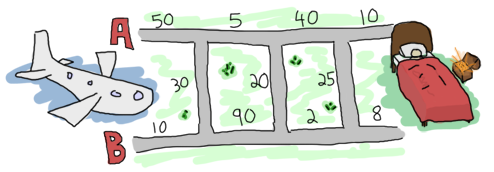
\includegraphics[width=0.7\textwidth]{road1.png}
\end{figure}

Так как после прочтения нескольких онлайн\--книг вы стали ярым фанатом Erlang\--а, то, конечно же, хотите решить эту задачу на вашем любимом языке.
Чтобы облегчить работу с картой, вы сохраняете исходные данные в файле \href{http://learnyousomeerlang.com/static/erlang/road.txt}{road.txt} следующим образом:
\begin{lstlisting}[style=erlang]
50
10
30
5
90
20
40
2
25
10
8
0
\end{lstlisting}

Информация о дороге организована по шаблону:
\ops{A1, B1, X1, A2,}\ops{ B2, X2, ..., An, Bn, Xn}, где \emph{x} \--- это один из переулков, соединяющих между собой части А и B.
В качестве последнего сегмента \emph{x} мы используем 0, так как в этот момент мы гарантированно будем находиться в пункте назначения.
Данные можно организовать в кортежи по 3 элемента (тройки) вида \ops{\{A,B,X\}}.

И тут вы понимаете, что если вы не знаете как решить эту задачу вручную, то нечего даже пытаться решить её на Erlang.
Для анализа задачи будем использовать то, чему нас научила рекурсия.

Первым шагом мы пытаемся найти частный случай.
Для нашей задачи это ситуация, когда осталось проанализировать лишь один кортеж, то есть сделать выбор между \emph{A, B} (и переулком \emph{x}, который в данном случае бесполезен, так как мы находимся в пункте назначения):
\begin{figure}[h!]
    \centering
    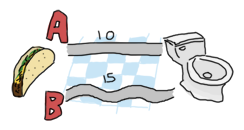
\includegraphics[width=0.5\textwidth]{road2.png}
\end{figure}

Поэтому остаётся лишь определить, какой путь короче: путь A или путь B.
Если вы хорошо изучили рекурсию, то знаете, что мы обязаны сходиться к частному случаю, то есть на каждом шаге мы будем пытаться свести задачу к выбору между A и B.

Расширим нашу карту и начнём заново:
\begin{figure}[h!]
    \centering
    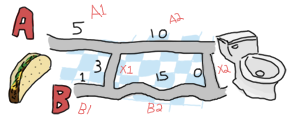
\includegraphics[width=0.5\textwidth]{road3.png}
\end{figure}

О, это уже интереснее!
Как мы можем перейти от тройки \ops{\{5,1,3\}} к чёткому выбору между A и B?
Определим, сколько существует вариантов для A.
Чтобы добраться до пересечения \emph{A1} и \emph{A2} (я буду называть это место \emph{точкой A1}), я могу поехать напрямую по дороге \emph{A1} (5), либо проехать по \emph{B1} (1), а затем по переулку \emph{X1} (3).
В этом случае первый вариант (5) длиннее второго (4).
Кратчайший путь для варианта А это \ops{[B, X]}.
А какие есть варианты для B?
Можно проехать по \emph{A1} (5), затем по переулку \emph{X1} (3), или сразу же избрать путь \emph{B1} (1).

Хорошо!
У нас есть путь длины 4 \ops{[B, X]} до первого пересечения А, и путь длины 1 \ops{[B]} до пересечения \emph{B1} и \emph{B2}.
Теперь мы должны сделать выбор между второй точкой A (пересечение \emph{A2} и конечной точки \emph{X2}) и второй точкой B (пересечение \emph{B2} и \emph{X2}).
Предлагаю сделать то же самое, что и раньше.
Так как тексты здесь пишу я, то моё решение вам оспорить не удастся.
Ну что ж, продолжим!

Все возможные пути для этого случая можно найти таким же способом, как и в предыдущей ситуации.
До точки A мы можем добраться либо по пути \emph{A2} из \ops{[B, X]}, который даёт нам длину 14 (\ops{14 = 4 + 10}, либо по \emph{B2}, а затем \emph{X2} из точки \ops{[B]}, что даёт нам длину 16 (\ops{16 = 1 + 15 + 0}).
Очевидно, что путь \ops{[B, X, A]} лучше пути \ops{[B, B, X]}.
\begin{figure}[h!]
    \centering
    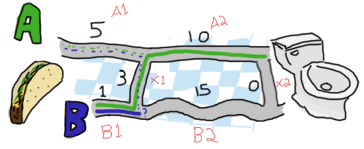
\includegraphics[width=0.7\textwidth]{road3_2.png}
\end{figure}

Также мы можем добраться до следующей точки B по пути \emph{A2} из \ops{[B, X]} и переулку \emph{X2}, что даст нам длину 14 (\ops{14 = 4 + 10 + 0}).
Либо по дороге \emph{B2} из \emph{[B]}, которая даст нам путь длины 16 (\ops{16 = 1 + 15}).
Мы выберем первый вариант: \ops{[B, X, A, X]}.

В конце у нас остаются два пути A и B.
Длина обоих равна 14.
Любой из этих маршрутов можно считать верным.
Окончательный  выбор всегда будет происходить между двумя маршрутами равной длины, если последний сегмент X имеет длину 0.
Наше рекурсивное решение даёт уверенность, что на выходе мы всегда получаем кратчайший путь.
Совсем неплохо, согласитесь.

Постепенно мы снабдили себя основными деталями, необходимыми для постройки рекурсивной функции.
Можете, конечно, её реализовать, если хотите, но я пообещал, что самостоятельно рекурсивные функции мы будем писать очень редко.
Здесь мы задействуем свёртку (fold).\\
\colorbox{lgray}
{
\begin{minipage}{1.0\linewidth}
    \textbf{Замечание:} хоть я и показывал, что свёртки используются для списков и создаются с их помощью, но свёртки представляют собой более универсальную концепцию перебора элементов структуры данных при помощи аккумулятора.
Поэтому свёртки можно реализовывать над деревьями, словарями (dictionaries), массивами, таблицами баз данных и т.д.

Во время экспериментов зачастую полезно использовать отображения (maps) и свёртки (folds).
С их помощью можно впоследствии легко изменить структуру данных, с которой работает логика вашей программы.
\end{minipage}
}

Итак, на чём мы остановились?
Ах, да!
Мы подготовили файл, который будем использовать как вход для нашей программы.
Для файловых манипуляций лучшим инструментом является \href{http://erldocs.com/R15B/kernel/file.html}{файловый модуль}.
Он содержит множество функций, которые встречаются в большинстве языков программирования и используются для работы с файлами (установка прав доступа, перемещение файлов, переименование и удаление и т.д.)

Модуль также содержит стандартные функции для чтения и/или записи из/в файлы, такие как \ops{\href{http://erldocs.com/R15B/kernel/file.html\#open/2}{file:open/2}} и \ops{\href{http://erldocs.com/R15B/kernel/file.html\#close/1}{file:close/1}}, которые делают именно то, о чём сообщают их имена (открывают и закрывают файлы!)
\ops{\href{http://erldocs.com/R15B/kernel/file.html\#read/2}{file:read/2}} извлекает из файла содержимое (в двоичном виде или в виде строки), \ops{\href{http://erldocs.com/R15B/kernel/file.html\#read\_line/1}{file:read\_line/1}} считывает единичную строку, \ops{\href{http://erldocs.com/R15B/kernel/file.html\#position/3}{file:position/3}} перемещает указатель в открытом файле в указанную позицию и т.д.

В модуле есть и несколько упрощённых функций, например \ops{\href{http://erldocs.com/R15B/kernel/file.html\#read\_file/1}{file:read\_file/1}} (открывает файл и читает его содержимое в двоичном виде), \ops{\href{http://erldocs.com/R15B/kernel/file.html\#consult/1}{file:consult/1}} (открывает и разбирает файл на термы Erlang) или \ops{\href{http://erldocs.com/R15B/kernel/file.html\#pread/2}{file:pread/2}} (меняет текущую позицию в файле, а потом считывает данные) и \ops{\href{http://erldocs.com/R15B/kernel/file.html\#pwrite/2}{pwrite/2}} (меняет текущую позицию и записывает данные).

С таким богатым выбором мы легко найдём функцию, которая позволит считать наш файл \href{http://learnyousomeerlang.com/static/erlang/road.txt}{road.txt}.
Так как нам известно, что описание дороги относительно невелико, то мы воспользуемся вызовом \ops{file:read\_file("road.txt").}:
\begin{lstlisting}[style=erlang]
1> {ok, Binary} = file:read_file("road.txt").
{ok,<<"50\r\n10\r\n30\r\n5\r\n90\r\n20\r\n40\r\n2\r\n25\r\n10\r\n8\r\n0\r\n">>}
2> S = string:tokens(binary_to_list(Binary), "\r\n\t ").
["50","10","30","5","90","20","40","2","25","10","8","0"]
\end{lstlisting}

Обратите внимание, что в данном случае я добавил пробел (\ops{'' ''\strut}) и символ табуляции (\ops{''\textbackslash t''}) в список валидных токенов, чтобы иметь возможность считывать файлы вида "50 10 30 5 90 20 40 2 25 10 8 0".
После считывания этого списка, нам нужно преобразовать строки в целые числа.
Применим способ, подобный тому, который мы использовали в нашем ОПЗ калькуляторе:
\begin{lstlisting}[style=erlang]
3> [list_to_integer(X) || X <- S].
[50,10,30,5,90,20,40,2,25,10,8,0]
\end{lstlisting}

Давайте создадим новый модуль, назовём его \href{http://learnyousomeerlang.com/static/erlang/road.erl}{road.erl} и запишем наши рассуждения в виде кода:
\begin{lstlisting}[style=erlang]
-module(road).
-compile(export_all).
 
main() ->
    File = "road.txt",
    {ok, Bin} = file:read_file(File),
    parse_map(Bin).
 
parse_map(Bin) when is_binary(Bin) ->
    parse_map(binary_to_list(Bin));
parse_map(Str) when is_list(Str) ->
    [list_to_integer(X) || X <- string:tokens(Str,"\r\n\t ")].
\end{lstlisting}

Функция \ops{main/0} отвечает за чтение содержимого файла и его передачу в функцию \ops{parse\_map/1}.
Так как для чтения мы используем функцию \ops{file:read\_file/1}, то полученный результат будет представлен в виде двоичных данных.
Поэтому я сделал так, чтобы функция \ops{parse\_map/1} проводила сопоставление и для списков, и для двоичных данных.
В случае двоичных данных мы просто повторно вызываем функцию и передаём ей строку, преобразованную в список (наша функция для разбиения строк работает только со списками).

Следующим шагом разбора данных, описывающих карту, будет перегруппировка чисел в кортежи \ops{\{A,B,X\}}, описанные ранее.
К сожалению, простого универсального способа выбрать из списка по 3 элемента за раз не существует, а поэтому нам придётся использовать сопоставление с образцом в рекурсивной функции:
\begin{lstlisting}[style=erlang]
group_vals([], Acc) ->
    lists:reverse(Acc);
group_vals([A,B,X|Rest], Acc) ->
    group_vals(Rest, [{A,B,X} | Acc]).
\end{lstlisting}

Эта функция оптимизируется в хвостовую рекурсию и ничего особенно сложного в ней не происходит.
Её нужно будет вызвать из слегка модифицированной функции \ops{parse\_map/1}:
\begin{lstlisting}[style=erlang]
parse_map(Bin) when is_binary(Bin) ->
    parse_map(binary_to_list(Bin));
parse_map(Str) when is_list(Str) ->
    Values = [list_to_integer(X) || X <- string:tokens(Str,"\r\n\t ")],
    group_vals(Values, []).
\end{lstlisting}

Если мы попробуем скомпилировать всё вместе, то получим осмысленное описание дороги:
\begin{lstlisting}[style=erlang]
1> c(road).
{ok,road}
2> road:main().
[{50,10,30},{5,90,20},{40,2,25},{10,8,0}]
\end{lstlisting}

Ага, похоже всё верно.
У нас появился ещё один элемент функции, которая потом попадёт в свёртку.
Теперь для осуществления задуманного нам нужен хороший аккумулятор.

Для выбора аккумулятора я использую следующий метод: представляю, что я внутри запущенного алгоритма.
Для этой конкретной задачи я представлю, что пытаюсь определить кратчайший путь для второй тройки (\ops{\{5,90,20\}}).
Чтобы определить лучший маршрут, мне нужно владеть результатом для предыдущей тройки.
К счастью, способ решения этой задачи нам уже известен, так как для него нам не понадобится аккумулятор, и всю необходимую логику мы уже записали.
Итак, для A:
\begin{figure}[h!]
    \centering
    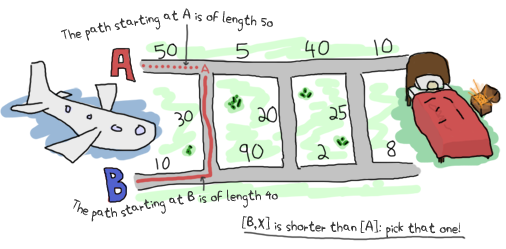
\includegraphics[width=0.85\textwidth]{road1_2.png}
\end{figure}

И из этих двух путей выбираем кратчайший.
\clearpage
Для B задача имеет похожее решение:
\begin{figure}[!htbp]
    \centering
    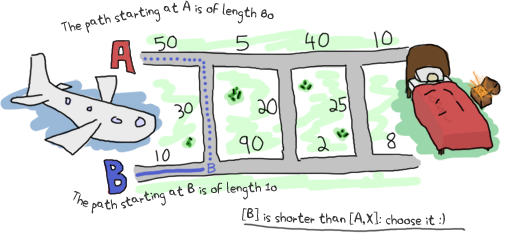
\includegraphics[width=0.85\textwidth]{road1_3.png}
\end{figure}

Теперь нам известно, что лучший путь в A на текущий момент \--- это \ops{[B,X]}.
Нам также известно, что его длина равна 40.
Оптимальный путь для B \--- просто \ops{[B]} и его длина 10.
Эту информацию мы можем использовать, чтобы найти следующий лучший маршрут для A и B, применяя похожие рассуждения, но при этом учитывая предыдущие решения.
Нам также пригодится пройденный путь, чтобы мы его могли показывать пользователю.
Необходимо найти два пути (один для A, второй для B) и две аккумулированные длины, поэтому аккумулятор можно выразить в виде кортежа \ops{\{\{DistanceA, PathA\}, \{DistanceB, PathB\}\}}.
Таким образом, каждая итерация свёртки имеет полный доступ к состоянию, и мы накапливаем результат, чтобы в конце показать его пользователю.

Теперь у нашей функции есть все необходимые параметры: тройки вида \ops{\{A,B,X\}} и аккумулятор \ops{\{\{DistanceA,PathA\}, \{DistanceB,PathB\}\}}.

Аккумулятор можно получить при помощи следующего кода:
\begin{lstlisting}[style=erlang]
shortest_step({A,B,X}, {{DistA,PathA}, {DistB,PathB}}) ->
    OptA1 = {DistA + A, [{a,A}|PathA]},
    OptA2 = {DistB + B + X, [{x,X}, {b,B}|PathB]},
    OptB1 = {DistB + B, [{b,B}|PathB]},
    OptB2 = {DistA + A + X, [{x,X}, {a,A}|PathA]},
    {erlang:min(OptA1, OptA2), erlang:min(OptB1, OptB2)}.
\end{lstlisting}

Переменной \emph{OptA1} присваивается первый вариант для A (перебираются элементы \emph{A}), переменной \emph{OptA2} \--- второй вариант (проходим по \emph{B}, затем по \emph{X}).
Для точки из B производим похожие манипуляции с переменными \emph{OptB1} и \emph{OptB2}.
В результате возвращаем аккумулятор с полученным маршрутом.

Заметьте, что для хранения маршрутов я решил использовать представление \ops{[\{x,X\}]} вместо \ops{[x]}, чтобы пользователь имел возможность узнать длину каждого сегмента.
Стоит также обратить внимание на то, что я накапливаю пути в обратном порядке (\ops{\{x,X\}} перед \ops{\{b,B\}}).
Это происходит из\--за того, что свёртка использует хвостовую рекурсию: весь список разворачивается задом\--наперёд, поэтому необходимо размещать последний пройденный элемент впереди остальных.

И, наконец, я использую функцию \ops{erlang:min/2}, чтобы найти кратчайший путь.
Применение этой функции сравнения к кортежам может показаться странным, но вспомните: каждый терм Erlang можно сравнивать с любым другим!
Благодаря тому, что первым элементом кортежа является длина, мы можем их сортировать.

Осталось вставить эту функцию в свёртку:
\begin{lstlisting}[style=erlang]
optimal_path(Map) ->
    {A,B} = lists:foldl(fun shortest_step/2, {{0,[]}, {0,[]}}, Map),
    {_Dist,Path} = if hd(element(2,A)) =/= {x,0} -> A;
            hd(element(2,B)) =/= {x,0} -> B
        end,
    lists:reverse(Path).
\end{lstlisting}

В результате выполнения свёртки, оба пути имеют одинаковую длину, но один из путей проходит через последний сегмент \ops{\{x,0\}}.
В конструкции \ops{if} мы смотрим на последний элемент обоих путей и возвращаем путь, который не проходит через \ops{\{x,0\}}.
Можно также просто выбрать путь с наименьшим числом шагов (сравнить результаты \ops{length/1}).
Как только кратчайший путь был найден, мы разворачиваем его задом\--наперёд (так как он был построен при помощи хвостовой рекурсии, его \textbf{нужно} развернуть).
Теперь маршрут можно показать всему миру или держать в секрете, чтобы заполучить богатое дядюшкино наследство.
Для успешной компиляции кода нужно добавить в функцию main вызов \ops{optimal\_path/1}.
\begin{lstlisting}[style=erlang]
main() ->
    File = "road.txt",
    {ok, Bin} = file:read_file(File),
    optimal_path(parse_map(Bin)).
\end{lstlisting}

О, глядите\--ка!
Мы получили верный ответ!
Отличная работа!
\begin{lstlisting}[style=erlang]
1> c(road).
{ok,road}
2> road:main().
[{b,10},{x,30},{a,5},{x,20},{b,2},{b,8}]
\end{lstlisting}

\begin{figure}[h!]
    \centering
    \includegraphics[width=0.7\textwidth]{road1_4.png}
\end{figure}

А знаете что ещё бы нам пригодилось?
Возможность запускать программу вне оболочки Erlang.
Опять слегка изменим нашу функцию main:
\begin{lstlisting}[style=erlang]
main([FileName]) ->
    {ok, Bin} = file:read_file(FileName),
    Map = parse_map(Bin),
    io:format("~p~n",[optimal_path(Map)]),
    erlang:halt().
\end{lstlisting}

Теперь арность функции main равна 1.
Это позволит нам получить параметры командной строки.
Я добавил вызов функции \ops{\href{http://erldocs.com/R15B/erts/erlang.html\#halt/0}{erlang:halt/0}}, после которого виртуальная машина Erlang завершает работу, и завернул вызов \ops{optimal\_path/1} в \ops{io:format/2}, потому что вне оболочки Erlang текст можно отобразить только таким способом.

С этими поправками файл \href{http://learnyousomeerlang.com/static/erlang/road.erl}{road.erl} примет следующий вид (не учитывая комментарии):
\begin{lstlisting}[style=erlang]
-module(road).
-compile(export_all).
 
main([FileName]) ->
    {ok, Bin} = file:read_file(FileName),
    Map = parse_map(Bin),
    io:format("~p~n",[optimal_path(Map)]),
    erlang:halt(0).
 
%% Transform a string into a readable map of triples
parse_map(Bin) when is_binary(Bin) ->
    parse_map(binary_to_list(Bin));
parse_map(Str) when is_list(Str) ->
    Values = [list_to_integer(X) || X <- string:tokens(Str,"\r\n\t ")],
    group_vals(Values, []).
 
group_vals([], Acc) ->
    lists:reverse(Acc);
group_vals([A,B,X|Rest], Acc) ->
    group_vals(Rest, [{A,B,X} | Acc]).
 
%% Picks the best of all paths, woo!
optimal_path(Map) ->
    {A,B} = lists:foldl(fun shortest_step/2, {{0,[]}, {0,[]}}, Map),
    {_Dist,Path} = if hd(element(2,A)) =/= {x,0} -> A;
                    hd(element(2,B)) =/= {x,0} -> B
                  end,
    lists:reverse(Path).
 
%% actual problem solving
%% change triples of the form {A,B,X}
%% where A,B,X are distances and a,b,x are possible paths
%% to the form {DistanceSum, PathList}.
shortest_step({A,B,X}, {{DistA,PathA}, {DistB,PathB}}) ->
    OptA1 = {DistA + A, [{a,A}|PathA]},
    OptA2 = {DistB + B + X, [{x,X}, {b,B}|PathB]},
    OptB1 = {DistB + B, [{b,B}|PathB]},
    OptB2 = {DistA + A + X, [{x,X}, {a,A}|PathA]},
    {erlang:min(OptA1, OptA2), erlang:min(OptB1, OptB2)}.
\end{lstlisting}

Исполним код:
\begin{lstlisting}[style=erlang]
$ erlc road.erl
$ erl -noshell -run road main road.txt
[{b,10},{x,30},{a,5},{x,20},{b,2},{b,8}]
\end{lstlisting}

Да, всё верно!
Для запуска программы больше ничего делать не нужно.
Эти две строки можно завернуть в единый bash/bat файл, или применить для этого \href{http://erlang.org/doc/man/escript.html}{escript}.

На примере этих двух упражнений мы увидели, что решать задачу становится проще, если сначала разбить её на мелкие части, по отдельности решить каждую подзадачу, а затем соединить всё воедино.
Мы также увидели, что нет смысла  начинать программирование до полного прояснения задачи.
Ну и несколько тестов, конечно же, никогда не будут лишними.
С их помощью вы убедитесь, что всё работает как положено и сможете менять код без изменения конечного результата.

\chapter{Краткий обзор общеизвестных структур данных}
\label{short-visit-to-common-data-structures}
\section{Обзор недолгий, обещаю!}
Функциональное подмножество Erlang вы, скорее всего, теперь понимаете достаточно неплохо, и текст многих программ смогли бы читать без проблем.
Но, тем не менее, готов поспорить, что вам не вполне ясно как построить настоящую полезную программу, хоть последняя глава и рассказывала о том, как решать задачи в функциональном стиле.
Говорю я об этом потому, что испытывал точно такие же чувства приблизительно в этот же момент моего обучения.
Впрочем, если у вас такой проблемы нет, то поздравляю!

В любом случае, я исхожу из того, что мы рассмотрели много всего: большинство базовых типов данных, оболочку, то как писать модули и функции (с рекурсией), различные способы компиляции, управление логикой программы, перехват исключений, абстракция некоторых общих операций и т.д.
Также мы познакомились с хранением данных в кортежах, списках, и рассмотрели незаконченную реализацию двоичного дерева поиска.
Но мы совсем не рассматривали другие структуры данных, которые предоставляет программисту стандартная библиотека Erlang.
\section{Записи}
\label{records}
\begin{wrapfigure}{r}{0.2\linewidth}
    \includegraphics[width=1\linewidth]{record-player.png}
\end{wrapfigure}
Прежде всего, записи \--- это хак.
Они \--- что\--то вроде запоздалой мысли, пришедшей в голову разработчикам языка, и поэтому имеют свои недостатки.
О недостатках я расскажу позже.
Записи очень пригождаются, если нам нужна небольшая структура данных, которая предоставляет прямой доступ к именованным атрибутам.
Поэтому записи в Erlang очень похожи на структуры в C (если вы знакомы с языком C).

Они объявляются так же как и атрибуты модуля:
\begin{lstlisting}[style=erlang]
-module(records).
-compile(export_all).
 
 -record(robot, {name,
                 type=industrial,
                 hobbies,
                 details=[]}).
\end{lstlisting}

Эта запись представляет информацию о роботе и имеет 4 поля: имя, тип робота, его хобби и подробности.
Для полей, хранящих тип и подробности, кроме того, задано значение по умолчанию: соответственно \ops{industrial} и \ops{[]}.
Вот так в модуле \href{http://learnyousomeerlang.com/static/erlang/records.erl}{records} можно объявить запись:
\begin{lstlisting}[style=erlang]
first_robot() ->
    #robot{name="Mechatron",
        type=handmade,
        details=["Moved by a small man inside"]}.
\end{lstlisting}

Запускаем код:
\begin{lstlisting}[style=erlang]
1> c(records).
{ok,records}
2> records:first_robot().
{robot,"Mechatron",handmade,undefined,
    ["Moved by a small man inside"]}
\end{lstlisting}

Опа!
Вот и хак!
Записи в Erlang \--- всего лишь синтаксический сахар поверх кортежей.
К счастью, ситуацию можно улучшить.
В оболочке Erlang есть команда \ops{rr(Module)}, которая позволяет загружать определения записей из \emph{Module}:
\begin{lstlisting}[style=erlang]
3> rr(records).
[robot]
4> records:first_robot().        
#robot{name = "Mechatron",type = handmade,
    hobbies = undefined,
    details = ["Moved by a small man inside"]}
\end{lstlisting}

Совсем другое дело!
Так с записями намного легче работать.
Вы можете заметить, что в \ops{first\_robot/0} мы не определяли поле \ops{hobbies}, и в его определении не было значения по умолчанию.
Erlang неявно присваивает неинициализированным полям значение undefined.

Следующая функция поможет нам увидеть, как ведут себя значения по умолчанию, установленные в определении записи \ops{robot}:
\begin{lstlisting}[style=erlang]
car_factory(CorpName) ->
    #robot{name=CorpName, hobbies="building cars"}.
\end{lstlisting}

И запускаем:
\begin{lstlisting}[style=erlang]
5> c(records).
{ok,records}
6> records:car_factory("Jokeswagen").
#robot{name = "Jokeswagen",type = industrial,
    hobbies = "building cars",details = []}
\end{lstlisting}

Теперь у нас есть промышленный робот, который любит заниматься постройкой машин.\\
\colorbox{lgray}
{
\begin{minipage}{1.0\linewidth}
    \textbf{Замечание:}  функция \ops{rr()} может принимать не только имя модуля, но и шаблоны (вида \ops{rr(''*'')}) и список загружаемых записей вторым аргументом.

    В оболочке есть ещё несколько функций, с помощью которых можно манипулировать записями: \ops{rd(Name, Definition)} позволяет определять запись способом похожим на \ops{-record(Name, Definition)}, который мы использовали в нашем модуле.
    Команду \ops{rf()} можно использовать для <<выгрузки>> всех записей, а \ops{rf(Name)} и \ops{rf([Names])} \--- чтобы избавиться только от указанных определений.

    Можно использовать команду \ops{rl()} для вывода определений всех записей в виде пригодном для непосредственного копирования в модуль, или её формы \ops{rl(Name)} и \ops{rl([Names])} для вывода лишь указанных записей.

    И, наконец, команда \ops{rp(Term)} конвертирует кортеж в запись (при условии, что запись пределена).
\end{minipage}
}

Но на одних записях далеко не уедешь.
Нужно уметь извлекать из них значения.
Делается это двумя способами.
Первый \--- специальный <<синтаксис с точкой>>.
Представим, что определение записи о роботе уже загружено:
\begin{lstlisting}[style=erlang]
5> Crusher = #robot{name="Crusher", hobbies=["Crushing people","petting cats"]}.
#robot{name = "Crusher",type = industrial,
    hobbies = ["Crushing people","petting cats"],
    details = []}
6> Crusher#robot.hobbies.
["Crushing people","petting cats"]
\end{lstlisting}

Синтаксис красотой не блещет.
Он выглядит так потому, что записи по природе своей \--- кортежи.
Не более чем уловка компилятора.
Поэтому для записи приходится хранить ключевые слова, которые определяют, к какой переменной она относится. Именно поэтому \ops{\#robot} \--- часть \ops{Crusher\#robot.hobbies}.
Всё это, конечно, огорчает, но ничего не поделаешь.
Вложенные записи выглядят ещё уродливее:
\begin{lstlisting}[style=erlang]
7> NestedBot = #robot{details=#robot{name="erNest"}}.
#robot{name = undefined,type = industrial,
    hobbies = undefined,
    details = #robot{name = "erNest",type = industrial,
                    hobbies = undefined,details = []}}
8> (NestedBot#robot.details)#robot.name.
"erNest"
\end{lstlisting}

И да, скобки обязательны.\\
\colorbox{lgray}
{
\begin{minipage}{1.0\linewidth}
    \textbf{Дополнение:} \\ 
    Начиная с ревизии R14A появилась возможность записывать вложенные записи без скобок.
    Вышеприведённый пример \emph{NestedBot} можно также записать как \ops{NestedRobot\#robot.details\#robot.name}.
    Работать такая запись будет аналогично.
\end{minipage}
}

Рассмотрим следующий пример, чтобы глубже обозначить зависимость записей от кортежей:
\begin{lstlisting}[style=erlang]
9> #robot.type.
3
\end{lstlisting}

Код выводит номер элемента кортежа, который реализует данное поле.

У записей есть одна оправдывающая их особенность \--- записи можно использовать в заголовках функции для сопоставления с образцом, а также в охранных выражениях.
Определите в начале файла новую запись, и добавьте несколько функций:
\begin{lstlisting}[style=erlang]
-record(user, {id, name, group, age}).
 
%% use pattern matching to filter
admin_panel(#user{name=Name, group=admin}) ->
    Name ++ " is allowed!";
admin_panel(#user{name=Name}) ->
    Name ++ " is not allowed".
 
%% can extend user without problem
adult_section(U = #user{}) when U#user.age >= 18 ->
    %% Show stuff that can't be written in such a text
    allowed;
adult_section(_) ->
    %% redirect to sesame street site
    forbidden.
\end{lstlisting}

В функции \ops{admin\_panel/1} показан синтаксис, который позволяет связывать переменную с любым полем записи (можно связывать переменные сразу с несколькими полями).
Следует отметить, что для связывания целой записи с переменной в функции \ops{adult\_section/1}, необходимо выполнить код \ops{SomeVar = \#some\_record\{\}}.
И, как обычно, скомпилировать:
\begin{lstlisting}[style=erlang]
10> c(records).
{ok,records}
11> rr(records).
[robot,user]
12> records:admin_panel(#user{id=1, name="ferd", group=admin, age=96}).
"ferd is allowed!"
13> records:admin_panel(#user{id=2, name="you", group=users, age=66}).
"you is not allowed"
14> records:adult_section(#user{id=21, name="Bill", group=users, age=72}).
allowed
15> records:adult_section(#user{id=22, name="Noah", group=users, age=13}).
forbidden
\end{lstlisting}

На этом примере можно увидеть, что нет необходимости делать сопоставление по всем элементам кортежа, или вообще иметь во время написания функции представление о количестве этих элементов.
Можно провести сопоставление только по возрасту или группе, а об остальных полях даже и не вспоминать.
Если бы нам пришлось использовать обычный кортеж, то определение функции выглядело бы приблизительно так: \ops{function(\{record, \_, \_, ICareAboutThis, \_, \_\}) -> \ldots}.
Как только кто\--либо решит добавить в кортеж новый элемент, кто\--то другой (скорее всего весьма недовольный этой ситуацией) будет обязан исправить все функции, в которых используется этот кортеж.

Эта функция показывает как обновлять запись (иначе пользы от них было бы мало):
\begin{lstlisting}[style=erlang]
repairman(Rob) ->
    Details = Rob#robot.details,
    NewRob = Rob#robot{details=["Repaired by repairman"|Details]},
    {repaired, NewRob}.
\end{lstlisting}

А затем:
\begin{lstlisting}[style=erlang]
16> c(records).
{ok,records}
17> records:repairman(#robot{name="Ulbert", hobbies=["trying to have feelings"]}).
{repaired,#robot{name = "Ulbert",type = industrial,
    hobbies = ["trying to have feelings"],
    details = ["Repaired by repairman"]}}
\end{lstlisting}

Как видите, моего робота починили.
Здесь для обновления записей используется особенный синтаксис.
Может показаться, что мы обновляем ту же самую запись (\ops{Rob\#robot\{Field=NewValue\}}), но на самом деле это просто уловки компилятора, которые маскируют скрытый вызов функции \ops{\href{http://erldocs.com/R15B/erts/erlang.html\#setelement/3}{erlang:setelement/3}}.

И последнее о записях.
Записи весьма полезны, а дублирование кода не очень.
Поэтому программисты на Erlang часто совмещают использование одних и тех же записей в нескольких модулях при помощи \emph{заголовочных файлов}.
Файл заголовков в Erlang очень похож на их аналог в языке C.
Это просто фрагмент кода, который добавляется в модуль, как будто он там был всегда.
Создайте файл \href{http://learnyousomeerlang.com/static/erlang/records.hrl}{records.hrl} и добавьте в него следующий код:
\begin{lstlisting}[style=erlang]
%% this is a .hrl (header) file.
-record(included, {some_field,
                  some_default = "yeah!",
                  unimaginative_name}).
\end{lstlisting}

Чтобы включить этот заголовок в \href{http://learnyousomeerlang.com/static/erlang/records.erl}{records.erl}, нужно просто добавить в модуль эту строчку:
\begin{lstlisting}[style=erlang,]
-include("records.hrl").
\end{lstlisting}

И в следующей функции применить запись:
\begin{lstlisting}[style=erlang]
included() -> #included{some_field="Some value"}.
\end{lstlisting}

А теперь, как обычно, проверим:
\begin{lstlisting}[style=erlang]
18> c(records).
{ok,records}
19> rr(records).
[included,robot,user]
20> records:included().
#included{some_field = "Some value",some_default = "yeah!",
         unimaginative_name = undefined}
\end{lstlisting}

Ура!
Довольно о записях.
Они, конечно,  неприятные, но полезные.
У них некрасивый синтаксис, они реализованы при помощи хака, но они играют сравнительно важную роль в удобстве поддержки вашего кода.\\
\colorbox{lgray}
{
\begin{minipage}{1.0\linewidth}
    \textbf{Замечание:} в проектах с открытым кодом вы сможете часто встретить описанный здесь метод.
В проект добавляется \ops{.hrl} файл, содержащий записи, которые используются во всех модулях приложения.
Хоть я и считаю, что обязан задокументировать этот способ использования записей, но я настоятельно рекомендую применять только локальные определения, которые действуют в пределах одного модуля.
Если вам нужно, чтобы какой\--либо другой модуль имел доступ к внутренему устройству записи \--- напишите несколько функций, которые предоставляют доступ к полям, а подробности реализации сделайте как можно более закрытыми.
Это правило позволяет предотвратить конфликт имён, помогает избежать проблем с обновлением кода, просто улучшает общую читабельность и упрощает поддержку вашего кода.
\end{minipage}
}
\section{Хранилища пар ключ\--значение}
\label{key-value-stores}
Несколько глав назад вы построили дерево и собирались его использовать в качестве хранилища пар ключ\--значение для адресной книги.
Книга получилась хреновая: удалять значения из неё мы не могли, да и найти ей достойное применение тоже не получилось.
С её помощью нам удалось хорошо продемонстрировать принцип работы рекурсии, но не более.
Пришло время познакомить вас с несколькими полезными структурами, предназначение которых \--- хранение данных, связанных с определённым ключом.
Я не буду рассказывать подробно о каждой функции, или делать полный обзор модулей.
Я просто дам вам ссылку на страницы документации.
Считайте, что моей обязанностью является <<улучшение осведомлённости о хранилищах пар ключ\--значение в Erlang>> или что\--то вроде того.
Ну а что, звание звучит неплохо.
Осталось только нашивку сделать.
\begin{wrapfigure}{r}{0.2\linewidth}
    \includegraphics[width=1\linewidth]{key.png}
\end{wrapfigure}

Для небольших объёмов данных можно использовать два вида структур.
Первая называется \emph{proplist} (список свойств).
Proplist \--- это любой список кортежей вида \ops{[\{Key, Value\}]}.
На этом правила, определяющие её устройство, заканчиваются.
Немного странная структура.
Список может также содержать булевы значения, целые числа и вообще всё что вам угодно.
Но сейчас нас интересует именно список, наполненный кортежами с ключом и значением.
Для работы с proplist\--ами можно использовать модуль \href{http://erldocs.com/R15B/stdlib/proplists.html}{proplists}.
Он содержит функции \ops{\href{http://erldocs.com/R15B/stdlib/proplists.html\#delete/2}{proplists:delete/2}}, \ops{\href{http://erldocs.com/R15B/stdlib/proplists.html\#get\_value/2}{proplists:get\_value/2}}, \ops{\href{http://erldocs.com/R15B/stdlib/proplists.html\#get\_all\_values/2}{proplists:get\_all\_values/2}}, \ops{\href{http://erldocs.com/R15B/stdlib/proplists.html\#lookup/2}{proplists:lookup/2}} и \ops{\href{http://erldocs.com/R15B/stdlib/proplists.html\#lookup\_all/2}{proplists:lookup\_all/2}}.

Вы заметите, что в этом списке нет функций для добавления и удаления элементов.
Это даёт представление о том, насколько нечётко определены proplist\--ы как структура данных.
Чтобы получить возможность добавлять и удалять элементы, придётся вручную добавлять их при помощи конструктора (\ops{[NewElement|OldList]}) и использовать, например, функцию \ops{\href{http://erldocs.com/R15B/stdlib/lists.html\#keyreplace/4}{lists:keyreplace/4}}.
Для работы с одной небольшой структурой данных приходится использовать два модуля, и это решение не назовёшь кристально чистым.
Но благодаря нечёткому определению proplist\--ов, их часто используют для представления списка настроек или общего описания какого\--либо предмета.
Proplist\--ы нельзя назвать полной структурой данных.
Их скорее можно отнести к общему шаблону, который используется для представления некоторого объекта или предмета при помощи списков и кортежей.
А модуль proplists \--- что\--то вроде инструментария поверх этого шаблона.

Если вам понадобилось хранилище пар ключ\--значение для небольших объёмов данных c более полной функциональностью, то модуль \href{http://erldocs.com/R15B/stdlib/orddict.html}{orddict} \--- это то что нужно.
Orddict\--ы (упорядоченные словари) \--- это proplist\--ы со склонностью к формализму.
Каждый ключ может присутствовать в структуре только один раз, список упорядочивается для ускорения поиска и т.д.
Обычные CRUD\--операции представлены функциями \ops{\href{http://erldocs.com/R15B/stdlib/orddict.html\#store/3}{orddict:store/3}}, \ops{\href{http://erldocs.com/R15B/stdlib/orddict.html\#find/2}{orddict:find/2}} (на случай, если вам точно не известно, есть ли такой ключ в словаре), \ops{\href{http://erldocs.com/R15B/stdlib/orddict.html\#fetch/2}{orddict:fetch/2}} (когда вы знаете, что такой ключ в словаре присутствует, или что он там \textbf{должен} быть) и \ops{\href{http://erldocs.com/R15B/stdlib/orddict.html\#erase/2}{orddict:erase/2}}.
\begin{wrapfigure}{l}{0.35\linewidth}
    \includegraphics[width=1\linewidth]{dict.png}
\end{wrapfigure}

Orddict\--ы представляют собой неплохой компромисс между сложностью и эффективностью, при условии, что количество элементов приблизительно равно 75 (ознакомьтесь с \href{http://learnyousomeerlang.com/static/erlang/keyval\_benchmark.erl}{моими замерами}).
Если количество элементов превышает это число, то вам нужно переключиться на какое\--либо другое хранилище пар ключ\--значение.

В принципе, существует два модуля/структуры для работы с большими объёмами данных: \href{http://erldocs.com/R15B/stdlib/dict.html}{dicts} и \href{http://erldocs.com/R15B/stdlib/gb\_trees.html}{gb\_trees}.
У словарей такой же интерфейс как и у orddict\--ов: \ops{\href{http://erldocs.com/R15B/stdlib/dict.html\#store/3}{dict:store/3}}, \ops{\href{http://erldocs.com/R15B/stdlib/dict.html\#find/2}{dict:find/2}}, \ops{\href{http://erldocs.com/R15B/stdlib/dict.html\#fetch/2}{dict:fetch/2}}, \ops{\href{http://erldocs.com/R15B/stdlib/dict.html\#erase/2}{dict:erase/2}} и любая другая функция, например \ops{\href{http://erldocs.com/R15B/stdlib/dict.html\#map/2}{dict:map/2}} и \ops{\href{http://erldocs.com/R15B/stdlib/dict.html\#fold/2}{dict:fold/2}} (их очень удобно использовать при работе с целой структурой).
Так что если вам нужно расширить orddict \--- словари очень хорошо справятся с этой задачей..

Зато у сбалансированных деревьев общего назначения есть несколько функций, которые предоставляют прямой доступ к управлению структурой.
По сути, у gb\_trees есть два режима: в первом режиме вам известно о структуре всё (я называю этот режим <<умным (smart) режимом>>), и второй, в котором вы не можете делать какие\--либо предположения о структуре (я называю этот режим <<наивным (naive) режимом>>).
В наивном режиме доступны функции \ops{\href{http://erldocs.com/R15B/stdlib/gb\_trees.html\#enter/2}{gb\_trees:enter/2}}, \ops{\href{http://erldocs.com/R15B/stdlib/gb\_trees.html\#lookup/2}{gb\_trees:lookup/2}} и \ops{\href{http://erldocs.com/R15B/stdlib/gb\_trees.html\#delete\_any/2}{gb\_trees:delete\_any/2}}.
В умном режиме им соответствуют функции \ops{\href{http://erldocs.com/R15B/stdlib/gb\_trees.html\#insert/3}{gb\_trees:insert/3}}, \ops{\href{http://erldocs.com/R15B/stdlib/gb\_trees.html\#get/2}{gb\_trees:get/2}}, \ops{\href{http://erldocs.com/R15B/stdlib/gb\_trees.html\#update/3}{gb\_trees:update/3}} и \ops{\href{http://erldocs.com/R15B/stdlib/gb\_trees.html\#delete/2}{gb\_trees:delete/2}}.
Ещё можно использовать \ops{\href{http://erldocs.com/R15B/stdlib/gb\_trees.html\#map/2}{gb\_trees:map/2}}, а такая возможность никогда не бывает лишней.

Недостатком <<наивных>> функций, в сравнении с <<умными>> является то, что после вставки нового элемента (или удаления нескольких), может появиться необходимость перебалансировки дерева.
Это займёт определённое время и потребует некоторого количества памяти (даже если просто нужно будет убедиться в том, что перебалансировка не нужна).
Все <<умные>> функции предполагают, что искомый ключ присутствует в дереве.
Это позволяет пропустить все проверки и уменьшает время исполнения операций.

Когда же всё\--таки необходимо использовать gb\_trees вместо dict?
Решение не вполне очевидно.
Результаты исполнения моего \href{http://learnyousomeerlang.com/static/erlang/keyval\_benchmark.erl}{измерительного модуля}, свидетельствуют о том, что gb\_trees и dicts показывают во многих случаях приблизительно одинаковый результат.
Но измерения также говорят о том, что dicts показывает самую высокую скорость при считывании значений, а gb\_trees отрабатывает немного быстрее в других операциях.
Вы cможете делать выбор, отталкиваясь от того, какие операции для вашей задачи важнее других.

Да, ещё запомните, что у dicts есть функция свёртки (fold), а у gb\_trees \--- нет.
Вместо неё у gb\_trees есть функция\--\emph{итератор}, которая возвращает часть дерева, к которой можно применить вызов \ops{gb\_trees:next(Iterator)} и получить следующее по порядку значение.
Так что к структуре gb\_trees не получится применять универсальный fold, а придётся писать собственные рекурсивные функции.
Зато gb\_trees предоставляет быстрый доступ к наименьшему и наибольшему элементу в структуре при помощи функций \ops{\href{http://erldocs.com/R15B/stdlib/gb\_trees.html\#smallest/1}{gb\_trees:smallest/1}} и \ops{\href{http://erldocs.com/R15B/stdlib/gb\_trees.html\#largest/1}{gb\_trees:largest/1}}.

Можно сказать, что при выборе хранилища пар ключ\--значение вы должны руководствоваться нуждами вашего приложения.
На ваше решение могут оказать влияние различные факторы, каждый из которых по\--своему важен: сколько данных вам необходимо хранить, какие операции с этими данными нужно выполнять и прочее.
Чтобы убедиться в том, что вы не ошиблись \--- проводите измерения, профилируйте код, сравнивайте скорость исполнения.\\
\colorbox{lgray}
{
\begin{minipage}{1.0\linewidth}
    \textbf{Замечание:} существуют специальные хранилища пар ключ\--значение для работы с ресурсами различного размера.
    Это \href{http://erldocs.com/R15B/stdlib/ets.html}{ETS таблицы}, \href{http://erldocs.com/R15B/stdlib/dets.html}{DETS таблицы} и база данных \href{http://erldocs.com/R15B/mnesia/mnesia.html?search=mnesia&i=0}{mnesia}.
    Но так как их использование тесно связано с концепцией множественных процессов и распределённостью, мы затронем их позже.
    Я оставляю эту информацию как ориентир, призванный разжечь ваше любопытство и направить заинтересовавшихся в нужном направлении.
\end{minipage}
}
\section{Массивы}
\label{arrays}
А как быть с кодом, для которого нужны структуры данных, принимающие только числовые данные?
В нём можно использовать \href{http://erldocs.com/R15B/stdlib/array.html}{массивы}.
К их элементам можно обращаться при помощи числовой идексации, а также применять ко всей структуре операцию свёртки.
При этом есть возможность игнорировать позиции с неопределённым значением.
\colorbox{lorange}
{
    \begin{minipage}{1.0\linewidth}
        \textbf{Не забывайтесь:}\\
В противоположность своим императивным собратьям, массивы Erlang не могут выполнять операции вставки и поиска за константное время.
На практике массивы используют редко, так как они обычно медленнее массивов в языках, подерживающих деструктивное присваивание, и стиль программирования на Erlang не очень хорошо стыкуется с массивами и матрицами.\\
В задачах, где необходимо использовать матричные манипуляции и массивы, программисты склоняются к использованию концепции, которая называется \href{http://www.erlang.org/doc/tutorial/c\_port.html}{Ports}.
С её помощью исполнение тяжёлых операций перекладывается на другие языки.
К той же концепции можно отнести \href{http://www.erlang.org/doc/tutorial/cnode.html}{C-Nodes}, \href{http://www.erlang.org/doc/tutorial/c\_portdriver.html}{Linked in drivers} и \href{http://erldocs.com/R15B/erts/erl\_nif.html}{NIF} (экспериментальная поддержка в R13B03+).\\
Ещё одна странность массивов заключается в том, что их индексация начинается с 0 (в противоположность кортежам или спискам).
Такая же индексация используется и в \href{http://erldocs.com/R15B/stdlib/re.html}{модуле для работы с регулярными выражениями}.
Будьте внимательны.
    \end{minipage}
}
\section{Набор наборов}
\label{a-set-of-sets}
\begin{wrapfigure}{r}{0.38\linewidth}
    \includegraphics[width=1\linewidth]{swingset.png}
\end{wrapfigure}
Если вам когда\--либо приходилось изучать теорию множеств, то у вас есть представление о свойствах наборов.
Если не приходилось, то вы, возможно, не захотите читать дальше.
Но я, всё\--таки скажу, что наборы \--- это группы уникальных элементов, которые можно сравнивать.
Над ними также можно совершать  различные действия: найти элементы, которые одновременно принадлежат двум группам, или не принадлежат ни одной группе, или принадлежат лишь одной из групп и т.д.
Можно также производить более сложные операции, которые позволяют определить связи между группами, совершать над ними действия, и ещё много всего.
Не буду погружаться в теорию (опять же, она выходит за рамки этой книги), а просто опишу наборы как они есть.

В Erlang существует 4 основных модуля, предназначенных для работы с наборами.
Сперва такое обилие может показаться странным, но оно порождено согласием разработчиков, что <<лучшего>> способа реализации наборов не существует.
Вот эти четыре модуля: \href{http://erldocs.com/R15B/stdlib/ordets.html}{ordsets}, \href{http://erldocs.com/R15B/stdlib/sets.html}{sets}, \href{http://erldocs.com/R15B/stdlib/gb\_sets.html}{gb\_sets} и \href{http://erldocs.com/R15B/stdlib/sofs.html}{sofs} (наборы наборов):

\begin{minipage}{1.0\linewidth}
    \textbf{ordsets}\\
    Ordset\--ы реализованы в виде упорядоченного списка.
    Главным образом, их хорошо использовать для небольших объёмов данных, и они \--- самый медленный вид набора.
    Но из всех наборов они имеют самый простой и легкочитаемый способ представления.
    Для них реализованы следующие стандартные функции: \ops{\href{http://erldocs.com/R15B/stdlib/ordsets.html\#new/0}{ordsets:new/0}}, \ops{\href{http://erldocs.com/R15B/stdlib/ordsets.html\#is\_element/2}{ordsets:is\_element/2}}, \ops{\href{http://erldocs.com/R15B/stdlib/ordsets.html\#add\_element/2}{ordsets:add\_element/2}}, \ops{\href{http://erldocs.com/R15B/stdlib/ordsets.html\#del\_element/2}{ordsets:del\_element/2}}, \ops{\href{http://erldocs.com/R15B/stdlib/ordsets.html\#union/1}{ordsets:union/1}}, \ops{\href{http://erldocs.com/R15B/stdlib/ordsets.html\#intersection/1}{ordsets:intersection/1}} и другие.\\
    \\
    \textbf{sets}\\
    Модуль sets использует в своей основе структуру, очень похожую на ту, что используется в \ops{dict}.
    Sets реализует тот же самый интерфейс, что и ordsets, но по сравнению с ним намного лучше масштабируется.
    Как и словари, эту структуру очень удобно использовать для действий, требующих большого количества операций чтения, например для проверки вхождения какого\--либо элемента в набор.\\
    \\
    \textbf{gb\_sets}\\
    Этот модуль построен поверх сбалансированных деревьев, похожих на структуру, используемую в модуле gb\_trees.
    gb\_sets относится к sets так же как и gb\_tree к dict.
    Они быстрее в операциях отличных от чтения, и дают больше контроля над структурой.
    Модуль gb\_sets не только реализует тот же самый интерфейс, что sets и ordsets, но и дополняет его множеством функций.
    Как и в gb\_trees у вас есть умные (smart) и наивные (naive) функции, итераторы, быстрый доступ к наименьшему и наибольшему значению и т.д.\\
    \\
    \textbf{sofs}\\
    Наборы наборов (osfs) реализованы при помощи упорядоченных списков, скомпонованных с метаданными в кортеж.
    Этот модуль следует использовать, если вы хотите полностью управлять связями наборов, их объединениями, обеспечивать для наборов соблюдение типов и т.д.
    Если вам требуется именно математическая концепция наборов, а не <<просто>> группы уникальных элементов, то вам необходим  именно этот модуль.
\end{minipage}
\\
\colorbox{lorange}
{
    \begin{minipage}{1.0\linewidth}
        \textbf{Не забывайтесь:}\\
        Такое многообразие можно, конечно, рассматривать как преимущество, но детали реализации могут свести эти преимущества на нет.
        К примеру, gb\_sets, ordsets и sofs \--- все используют оператор \ops{==} для сравнения значений.
        Числа 2 и 2.0 при сравнении будут рассматриваться как одно и то же число.\\
        \\
        А вот, модуль sets использует оператор \ops{=:=}.
        Так что просто переключаться по желанию между реализациями получится не всегда.
        В некоторых случаях вам будет подходить лишь одно поведение, и тогда все преимущества, которые даёт множество реализаций, просто исчезнут.
    \end{minipage}
}

Такой широкий выбор немного сбивает с толку.
Разработчик Bj\"{o}rn Gustavsson из команды Erlang/OTP, который также разрабатывает \href{http://www.wings3d.com/}{Wings3D}, рекомендует в большинстве случаев использовать gb\_sets; ordset использовать, когда для последующей обработки в собственном коде необходимо простое представление данных, а sets оставить на случай, когда для сравнения нужно использовать оператор \ops{=:=} (\href{http://erlang.org/pipermail/erlang-questions/2010-March/050332.html}{источник}).

Как бы то ни было, обычно лучше провести замеры производительности вашего кода, и определить структуру, которая наилучшим образом подходит для вашей задачи.
\section{Ориентированные графы}
\label{directed-graphs}
Хочу упомянуть ещё одну структуру данных (я не хочу сказать, что помимо упомянутых в этой главе структур ничего больше нет, как раз наоборот): \href{http://en.wikipedia.org/wiki/Directed\_graph}{ориентированные графы}.
Эта структура, опять же, будет полезна читателям, знакомым с математической основой орграфов.

В Erlang взаимодействие с ориентированными графами реализуется двумя модулями: \href{http://erldocs.com/R15B/stdlib/digraph.html}{digraph} и \href{http://erldocs.com/R15B/stdlib/digraph\_utils}{digraph\_utils}.
Модуль digraph позволяет создавать и модифицировать орграфы: совершать манипуляции с рёбрами и вершинами, находить пути и циклы и т.д.
А digraph\_utils позволяет передвигаться по графу (прямой порядок, обратный порядок), проверять на наличие циклов, деревьев, находить соседние вершины и так далее.

Так как орграфы тесно связаны с теорией множеств \---  модуль <<sofs>> содержит несколько функций, которые позволяют конвертировать \href{http://erldocs.com/R15B/stdlib/sofs.html\#family\_to\_digraph/2}{семейства в орграфы} и \href{http://erldocs.com/R15B/stdlib/sofs.html\#digraph\_to\_family/2}{орграфы в семейства}.
\section{Очереди}
\label{queues}
Модуль \href{http://erldocs.com/R15B/stdlib/queue.html}{queue} реализует двунаправленную FIFO (\href{http://en.wikipedia.org/wiki/FIFO\_(computing)}{First In, First Out}) очередь:
\begin{figure}[h!]
    \centering
    \includegraphics[width=0.4\textwidth]{fifo.png}
\end{figure}
На картинке представлена примерная реализация: два списка (в этом контексте стеки), которые позволяют быстро добавлять элементы в голову и хвост очереди.

Модуль queue содержит несколько функций, которые мысленно можно отнести к 3\--м интерфейсам (или API) различной сложности.
Они называются <<Оригинальный API>>, <<Расширенный API>>, и <<Okasaki API>>:
\\

\begin{minipage}{1.0\linewidth}
    \textbf{Оригинальный API}\\
    Оригинальный API содержит функции, реализующие базовые свойства очереди.
    В их число входят: \ops{\href{http://erldocs.com/R15B/stdlib/queue.html\#new/0}{new/0}} создаёт пустую очередь, \ops{\href{http://erldocs.com/R15B/stdlib/queue.html\#in/2}{in/2}} вставляет новый элемент, \ops{\href{http://erldocs.com/R15B/stdlib/queue.html\#out/1}{out/1}} удаляет элемент. Здесь также есть функции для конвертации очереди в список, функция для изменения порядка элементов на противоположный, для определения вхождения какого\--либо значения в очередь и т.д.\\
    \\
    \textbf{Расширенный API}\\
    В расширенном API, главным образом, введены средства, придающие структуре гибкость, и позволяющие осуществлять интроспекцию.
    С их помощью можно, например, извлекать головной элемент без его удаления (см. \ops{\href{http://erldocs.com/R15B/stdlib/queue.html\#get/1}{get/1}} или \ops{\href{http://erldocs.com/R15B/stdlib/queue.html\#peek/1}{peek/1}}), просто удалять элементы, не заботясь об их значении (\ops{\href{http://erldocs.com/R15B/stdlib/queue.html\#drop/1}{drop/1}}), и т.д.
    Эти функции нельзя отнести к основам, составляющим концепцию очереди, но всё равно они весьма полезны.\\
    \\
    \textbf{Okasaki API}\\
    Okasaki API немного странный.
    Он взят из книги Chris Okasaki \href{http://books.google.ca/books?id=SxPzSTcTalAC&lpg=PP1&dq=chris\%20okasaki\%20purely\%20functional\%20data\%20structures&pg=PP1\#v=onepage&q=&f=false}{Purely Functional Data Structures}.
    Этот API предоставляет набор операций, похожий на предыдущие два, но некоторые имена функций в нём записываются задом\--наперёд, и в целом этот API весьма своеобразен.
    Если вы не вполне уверены, что вам нужен именно этот API, то лучше с ним не связывайтесь.\\
\end{minipage}

Очереди обычно используют, когда необходимо убедиться, что первый по порядку элемент точно будет обработан первым.
Те примеры, которые я показывал ранее, в качестве аккумуляторов в основном использовали списки, которые мы разворачивали в конце вычислений.
Если вы не можете развернуть сразу все элементы, или в аккумулятор приходится часто добавлять новые, то вам скорее всего нужен модуль queue (конечно же, вы сперва должны провести измерения и всё проверить!
Первым делом всё всегда нужно измерять и проверять!)
\section{Окончание краткого обзора}
Вот и закончен наш краткий экскурс в структуры данных Erlang.
Спасибо, что во время путешествия не высовывали руки за пределы транспортного средства.
Есть, конечно же, и другие структуры данных, которые помогают в решении различных задач.
Я осветил лишь те, которые вам пригодятся больше всех, и с которыми, учитывая специфику задач решаемых с помощью  Erlang, вы точно столкнётесь.
Для поиска дополнительных сведений рекомендую обратиться к \href{http://www.erlang.org/doc/apps/stdlib/index.html}{стандартной} и \href{http://www.erlang.org/doc/applications.html}{расширенной} библиотеке.

Вас наверняка порадует, что на этом мы завершаем путешествие в последовательный (sequential) (функциональный) Erlang.
Я знаком со многими людьми, которые начали изучать  Erlang из\--за параллелизма, процессов и всего прочего.
И это неудивительно, ведь Erlang блестяще справляется с задачами именно в этих областях.
К вашим услугам: деревья контроля, развитая система управления ошибками, распределённость и многое другое.
Знаю, что из\--за собственной нетерпеливости я уже касался этих тем, а некоторые нетерпеливые читатели уже наверняка о них успели прочитать.

Тем не менее, я посчитал, что перед переходом к параллельному Erlang нужно привыкнуть к его функциональной стороне.
Так нам будет легче продвигаться по материалу и концентрироваться лишь на новых концепциях.
Начинаем!
\begin{figure}[h!]
    \centering
    \includegraphics[width=0.7\textwidth]{squid-concurrency.png}
\end{figure}

\chapter{Путеводитель по параллелизму для путешествующих автостопом}
\label{the-hitchhikers-guide-to-concurrency}
Далеко\--далеко в закоулках нефешенебельного начала 21\--го века, которого даже нет на карте, находится маленькое подмножество человеческих знаний.

В этом подмножестве заключена совершенно невзрачная маленькая дисциплина, чья Фон\--Неймановская архитектура столь примитивна, что согласно ей ОПЗ калькуляторы считаются чем\--то выдающимся.

У этой дисциплины есть, а точнее была \--- проблема: большинство людей, изучающих её, были почти всегда недовольны, создавая параллельное ПО.
Предлагалось множество решений этой проблемы, но чаще всего они были связаны с манипуляцией маленькими логическими блоками, которые назывались локами, мутексами и всякими другими именами, что несколько странно, поскольку этим самым блокам параллелизм был совершенно не нужен.

Так проблема и оставалась нерешённой: одни люди были жадными, другие жалкими, и даже ОПЗ калькуляторы им не помогали.

Кое\--кто был убеждён, что людям не стоило добавлять параллелизм в языки программирования.
И что программы вообще не должны были выходить из их первоначального потока.
\\
\colorbox{lgray}
{
\begin{minipage}{1.0\linewidth}
    \textbf{Замечание:} неплохое развлечение \--- писать пародии на <<Путеводитель по галактике для путешествующих автостопом>>.
    Если вам ещё не попадалась эта книга, то обязательно её прочитайте.
    Она стоит того!
\end{minipage}
}
\section{Без паники}
\label{dont-panic}
\begin{wrapfigure}{l}{0.35\linewidth}
    \includegraphics[width=1\linewidth]{fat-guy.png}
\end{wrapfigure}
Привет.
Сегодня (или в любой из дней, когда вы читаете эти строки, даже завтра) я хочу рассказать вам о параллельном Erlang.
Скорее всего вы уже читали о параллелизме, или когда\--либо сталкивались с ним.
Может быть, вы интересуетесь истоками программирования для множества ядер, или читаете эту книгу, наслушавшись болтовни, которой в наше время окружён параллелизм.

Впрочем, хочу вас предупредить, что в этой главе основной упор сделан на теорию.
Если у вас болит голова, или вы питаете отвращение к истории языков программирования, или вам просто хотелось попрограммировать, то вам лучше перейти к ~\ref{thanks-for-all-the-fish}~концу главы, или перейти к следующей (там как раз освещается более практическая сторона вопроса).

Я уже объяснил во введении к книге, что параллелизм в Erlang основан на передаче сообщений и модели акторов.
Мой пример рассказывал о людях, общение которых происходит исключительно при помощи писем.
Чуть позже я ещё вернусь к этой модели, а сейчас нам необходимо первым делом обозначить разницу между \emph{конкурентностью} и \emph{параллелизмом}.

Оба слова во многих ситуациях имеют одно и то же значение.
Но в контексте Erlang они часто относятся к двум разным концепциям.
По мнению большинства эрлангистов понятие конкурентности описывает несколько акторов, которые исполняются независимо друг от друга, но их исполнение не обязательно происходит в один тот же момент.
Параллелизм же означает, что несколько акторов исполняются одновременно.
Взгляды различных областей computer science на правильность этих определений могут не совпадать, но в этом руководстве я буду пользоваться именно такими определениями.
Не удивляйтесь, если в других источниках вы увидите, как кто\--то употребляет те же самые термины для обозначения других понятий.

Конкурентность была в Erlang с самого начала, даже в восьмедисятые, когда всё запускалось на одноядерном процессоре.
Каждому процессу Erlang для исполнения отводился свой собственный временной отрезок, совсем как в эру десктопных приложений, которая предшествовала появлению многоядерных систем.

Уже в то время можно было, в принципе, реализовать параллелизм.
Для этого нам бы потребовался второй компьютер, который бы исполнял код и обменивался информацией с первым.
Но даже такая система могла бы исполнять параллельно всего лишь два актора.
Современные многоядерные системы позволяют реализовать параллелизм в рамках одного компьютера (некоторые промышленные чипы могут содержать десятки ядер), и Erlang использует эту возможность в полной мере.\\
\colorbox{lorange}
{
\begin{minipage}{1.0\linewidth}
    \textbf{Не забывайтесь:}\\
    Важно понимать разницу между конкурентностью и параллелизмом.
    Многие программисты верят, что Erlang был готов к использованию на многоядерных компьютерах задолго до того, как это произошло в действительности.
    Erlang стал использовать истинную \href{http://en.wikipedia.org/wiki/Symmetric\_multiprocessing}{симметричную мультипроцессорность} (symmetric multiprocessing) лишь в середине двухтысячных, а большая часть реализации была завершена в релизе R13B в 2009 году.
    До этого часто приходилось отключать SMP, чтобы избежать потерь производительности.
    На многоядерном компьютере без SMP можно получить параллелизм, если запустить одновременно несколько экземпляров виртуальной машины.\\
    \\
    Интересно отметить, что для внесения истинного параллелизма в язык, не потребовалось производить какие\--либо концептуальные изменения на языковом уровне.
    Благодаря тому, что конкурентность в Erlang строится вокруг изолированных процессов, все изменения были сделаны внутри ВМ, подальше от глаз обычного программиста.
\end{minipage}
}
\section{Принципы конкурентности}
\label{concepts-of-concurrency}
\begin{wrapfigure}{r}{0.35\linewidth}
    \includegraphics[width=1\linewidth]{erlang-the-movie.png}
\end{wrapfigure}
Когда\--то разработка языка Erlang проходила в быстром темпе, и от инженеров, которые занимались разработкой на Erlang для телефонных коммутаторов, поступал плотный поток обратной связи.
Их отчёты подтвердили, что конкурентность, основанная на процессах, и асинхронная передача сообщений позволяли хорошо моделировать задачи, возникающие перед разработчиками.
Кроме того, ещё до появления Erlang, в мире телефонии уже сформировалась некая культура, тяготеющая к параллелизму.
Она была унаследована от языка PLEX, который ранее был создан в Ericsson, и использовался в коммутаторах AXE.
Erlang унаследовал эту тенденцию, и попытался усовершенствовать существующие инструменты.

Для того, чтобы Erlang считался хорошим инструментом, он должен был удовлетворять нескольким требованиям.
Главным условием была возможность масштабирования и поддержки тысяч и тысяч пользователей на множестве коммутаторов.
И эти коммутаторы должны были обеспечивать высокую надёжность работы \--- вплоть до того, что исполнение кода никогда не должно было останавливаться.

\subsection{Масштабируемость}
\label{scalability}
Для начала я расскажу о масштабировании.
Для достижения масштабируемости была необходима система, обладающая определёнными свойствами.
В такой системе пользователи были бы представлены при помощи процессов, которые реагируют на определённые события (например, приём звонка, завершение разговора и т.д.).
Идеальная система должна поддерживать процессы, выполняющие малые объёмы вычислений, и быстрое переключение между процессами при поступлении событий. 
Высокоэффективная обработка процессов предполагала возможность их очень быстрого старта, очень быстрого уничтожения, и очень быстрой коммутации.
Обязательным условием для такого поведения была легковесность процессов.
Это было также необходимо, чтобы избавиться от наличия пула процессов (фиксированное множество процессов, между которыми распределяется работа).
Намного легче создавать программы, которые используют сразу столько процессов, сколько нужно.

Ещё один важный аспект масшабируемости \--- это возможность преодоления ограниченности ресурсов оборудования.
Для решения этой задачи выделяют два направления: можно улучшать характеристики оборудования, а можно увеличивать его количество.
Первое решение будет работать до определённого момента, после которого за улучшение придётся очень дорого платить (необходимо, например, покупать суперкомпьютер).
Второе решение, как правило, обходится дешевле.
Для выполнения тех же задач нужно просто добавлять больше компьютеров.
Вот где вашему языку может пригодиться распределённость.

Вернёмся к обсуждению лёгких процессов.
Высокая надёжность очень важна для нужд телефонии, поэтому разработчики решили, что правильнее всего будет запретить процессам иметь общую память.
Некоторые аварийные ситуации с участием разделяемой памяти могут привести к противоречивому состоянию (особенно если данные разделяются между несколькими узлами) и осложнениям.
Вместо этого процессы должны общаться при помощи сообщений, которые содержат полные копии данных.
Этим мы рискуем получить более медленное, но зато более безопасное решение.
\subsection{Устойчивость к сбоям}
\label{fault-tolerance}
Мы приходим ко второму требованию, которому должен соответствовать Erlang: надёжность.
Первые разработчики на Erlang всегда помнили о том, что сбои происходят повсеместно.
Можно сколько угодно пытаться предотвратить ошибки, но в большинстве случаев от некоторых из них не получится избавиться полностью.
И даже если не будет ошибок \--- от сбоев оборудования никуда не денешься.
Поэтому вместо того, чтобы пытаться полностью предотвратить ошибки, лучше найти хороший способ их обрабатывать.

Оказывается, что подход к проектированию при помощи множественных процессов с передачей сообщений, оказался верным, так как в него можно относительно легко встроить обработку ошибок.
Возьмём, к примеру, легковесные процессы (созданные для быстрых перезапусков и выключений).
Исследования показали, что для масштабных программных комплексов главным источником простоя являются ошибки, которые нерегулярно себя проявляют и спонтанно исчезают (\href{http://dslab.epfl.ch/pubs/crashonly/}{источник}).
Существует правило, говорящее что ошибки, которые искажают данные, должны как можно быстрее приводить к остановке неисправной части системы, чтобы предотвратить проникновение ошибок и плохих данных в остальные узлы.
Есть также ещё одна концепция, согласно которой существует множество различных способов остановки системы.
Двумя такими способами являются корректная остановка и сбой (завершение, вызванное непредвиденной ошибкой).

Очевидно, что наихудшим исходом будет сбой.
Для безопасного устранения проблемы сбоев можно сделать так, чтобы все аварийные ситуации проходили так же, как и корректные остановки.
Для этого необходимо использовать ряд методов, к которым можно отнести принцип неразделяемости ресурсов (shared-nothing) и единичное присваивание (single assignment) (которое позволяет изолировать память процесса), уход от \href{http://en.wikipedia.org/wiki/Lock_(computer_science)}{блокировок} (после аварии блокировка может остаться закрытой, и будет перекрывать другим процессам доступ к данным, или просто приводить данные в нестабильное состояние), а также другие техники, которые я не буду подробно описывать, но они также использовались при проектировании Erlang.
Таким образом, идеальным решением аварийной ситуации в Erlang считается быстрое уничтожение процессов, которое позволяет избежать порчи данных и случайных, нерегулярных ошибок.
Ключевым элементом этой схемы являются лёгкие процессы.
В языке также присутствуют механизмы обработки ошибок, которые позволяют процессам следить за другими процессами (подробнее о них в главе \ref{errors-and-processes}~Ошибки и процессы), определять момент смерти процесса и планировать действия, связанные с этим событием.

\chapter{Снова о многопроцессорности}
\section{Предъявите ваше состояние}
\begin{wrapfigure}{r}{0.35\linewidth}
    \includegraphics[width=1\linewidth]{turkey.png}
\end{wrapfigure}
Примеры, показанные в предыдущей главе, годились для использования в качестве демонстрационного материала, но с таким ограниченным инструментарием далеко не уйдёшь.
Нет, примеры плохими не назовёшь, но от процессов и акторов пользы мало, когда они представлены только функциями и сообщениями.
Для устранения этого недостатка нам необходимо уметь сохранять в процессе состояние.

Давайте, для начала, создадим функцию в новом модуле \href{http://learnyousomeerlang.com/static/erlang/kitchen.erl}{kitchen.erl}, которая позволит процессу выполнять функции холодильника.
Процессу разрешено совершать две операции: хранить еду в холодильнике и вынимать её оттуда.
Вынимать можно только ту еду, которая была заранее помещена в холодильник.
Пусть основой нашего процесса будет следующая функция:
\begin{lstlisting}[style=erlang]
-module(kitchen).
-compile(export_all).
 
 fridge1() ->
     receive
         {From, {store, _Food}} ->
         From ! {self(), ok},
         fridge1();
     {From, {take, _Food}} ->
         %% uh....
         From ! {self(), not_found},
         fridge1();
     terminate ->
         ok
     end.
\end{lstlisting}

Что\--то здесь не так.
Когда мы делаем запрос на хранение еды, процесс возвращает результат \emph{ok}, но фактически еда нигде не сохраняется.
Будет вызвана функция \emph{fridge1()}, и она начнёт исполняться с чистого листа, без сохранённого состояния.
Очевидно также, что когда мы просим процесс извлечь еду из холодильника, её просто неоткуда взять, и остаётся просто вернуть в качестве результата \emph{not\_found}.
Ясно, что для хранения и извлечения провизии нам необходимо добавить в функцию состояние.

Благодаря рекурсии, состояние процесса может целиком содержаться в параметрах, которые передаются в функцию.
Для нашего процесса\--холодильника можно хранить весь провиант в виде списка, и когда кто\--нибудь захочет поесть, мы сможем поискать в нём необходимый продукт:
\begin{lstlisting}[style=erlang]
fridge2(FoodList) ->
    receive
        {From, {store, Food}} ->
            From ! {self(), ok},
            fridge2([Food|FoodList]);
        {From, {take, Food}} ->
            case lists:member(Food, FoodList) of
                true ->
                    From ! {self(), {ok, Food}},
                    fridge2(lists:delete(Food, FoodList));
                false ->
                    From ! {self(), not_found},
                    fridge2(FoodList)
            end;
        terminate ->
            ok
    end.
\end{lstlisting}

Сразу можно заметить, что \ops{fridge2/1} принимает один аргумент \--- \emph{FoodList}.
Когда мы пошлём сообщение вида \ops{\{From, \{store, Food\}\}} \--- функция добавит значение \emph{Food} в \emph{FoodList} перед следующей итерацией.
На следующей итерации рекурсивного вызова можно будет извлечь из списка тот же самый элемент, который мы туда поместили ранее.
Я даже реализовал эту возможность.
Функция использует \ops{lists:member/2} для проверки наличия \ops{Food} в \ops{FoodList}.
В зависимости от результата, полученный элемент либо пересылается вызывающему процессу (и удаляется из \emph{FoodList}), либо получателю отсылается атом \emph{not\_found}:
\begin{lstlisting}[style=erlang]
1> c(kitchen).
{ok,kitchen}
2> Pid = spawn(kitchen, fridge2, [[baking_soda]]).
<0.51.0>
3> Pid ! {self(), {store, milk}}.
{<0.33.0>,{store,milk}}
4> flush().
Shell got {<0.51.0>,ok}
ok
\end{lstlisting}

Функция хранения продуктов в холодильнике вроде бы работает.
Теперь попробуем поместить туда различные продукты, а затем их извлечь.
\begin{lstlisting}[style=erlang]
5> Pid ! {self(), {store, bacon}}.
{<0.33.0>,{store,bacon}}
6> Pid ! {self(), {take, bacon}}.
{<0.33.0>,{take,bacon}}
7> Pid ! {self(), {take, turkey}}.
{<0.33.0>,{take,turkey}}
8> flush().
Shell got {<0.51.0>,ok}
Shell got {<0.51.0>,{ok,bacon}}
Shell got {<0.51.0>,not_found}
ok
\end{lstlisting}

В соответствии с нашими ожиданиями, мы можем достать из холодильника бекон, потому что мы его туда поместили первым по счёту (вместе с молоком и пищевой содой), но когда мы просим процесс\--холодильник достать немного мяса индейки, у него ничего не выходит.
Именно поэтому мы получаем последнее сообщение \ops{\{<0.51.0>,not\_found\}}.

\chapter{Ошибки и процессы}
\label{errors-and-processes}
\section{Связи}
\label{links}
Связи \--- это особый вид взаимоотношений, которые могут быть установлены между двумя процессами.
Когда один из процессов, который участвует в таких отношениях, умирает от неожиданного броска, ошибки или завершения (см. \ref{errors-and-exceptions} Ошибки и исключения), то связанный с ним процесс тоже завершается.

Эта концепция может пригодиться, когда требуется как можно быстрее завершить процесс, чтобы предотвратить появление ошибок.
Если процесс, в котором появилась ошибка, завершился аварией, а процессы, которые на него полагаются, продолжили работать, то все эти зависимые процессы должны что\--то предпринять.
Обычно приемлемым вариантом развития событий можно считать остановку и перезапуск всей группы процессов.
Именно это и позволяют нам сделать связи.

Для создания связи между двумя процессами в Erlang существует базовая функция \href{http://erldocs.com/R15B/erts/erlang.html\#link/1}{link/1}, принимающая в качестве аргумента Pid.
После запуска эта функция создаст связь между текущим процессом и процессом, который отождествляется с указанным \emph{Pid}.
Для разрушения связи используют функцию \href{http://erldocs.com/R15B/erts/erlang.html\#unlink/1}{unlink/1}.
При аварийном завершении одного из связанных процессов, отсылается сообщение особого вида, которое несёт информацию относительно произошедших событий.
Если процесс умирает по естественным причинам (читай: завершает исполнение своих функций), то такое сообщение не отсылается.
Для начала поговорим об этой новой функции как об элементе модуля \href{http://learnyousomeerlang.com/static/erlang/linkmon.erl}{linkmon.erl}:
\begin{lstlisting}[style=erlang]
myproc() ->
    timer:sleep(5000),
    exit(reason).
\end{lstlisting}

Если вы попробуете исполнить следущие вызовы функций (и сделаете между каждой командой spawn пятисекундную паузу), то увидите, что оболочка завершится с ошибкой 'reason' только если между двумя процессами была установлена связь.
\begin{lstlisting}[style=erlang]
1> c(linkmon).
{ok,linkmon}
2> spawn(fun linkmon:myproc/0).
<0.52.0>
3> link(spawn(fun linkmon:myproc/0)).
true
** exception error: reason
\end{lstlisting}

Изобразим это на картинке:
\begin{figure}[h!]
    \centering
    \includegraphics[width=0.7\textwidth]{link-exit.png}
\end{figure}

Для захвата сообщения \ops{\{'EXIT', B, Reason\}} не получится использовать стандартную структуру \ops{try \ldots catch}.
Для этого существуют другие средства, которые мы рассмотрим позже.

Важно отметить, что связи можно также использовать, для организации больших групп процессов, которые должны прекращать исполнения как единая группа, все вместе:
\begin{lstlisting}[style=erlang]
chain(0) ->
    receive
        _ -> ok
    after 2000 ->
        exit("chain dies here")
    end;
chain(N) ->
    Pid = spawn(fun() -> chain(N-1) end),
    link(Pid),
    receive
        _ -> ok
    end.
\end{lstlisting}

Эта функция принимает целое число \emph{N}, запускает \emph{N} связанных между собой процессов.
Для передачи \emph{N-1} аргумента следующему процессу в <<цепи>>, я оборачиваю вызов в анонимную функцию, чтобы она перестала принимать аргументы.
Подобный эффект можно получить при помощи вызова \ops{spawn(?MODULE, chain, [N-1])}.

В этом примере я создам множество связанных процессов, которые будут умирать сразу после завершения их наследников:
\begin{lstlisting}[style=erlang]
4> c(linkmon).              
{ok,linkmon}
5> link(spawn(linkmon, chain, [3])).
true
** exception error: "chain dies here"
\end{lstlisting}

Как видите, оболочка получает сообщение о смерти от одного из процессов.
Вот подробное описание завершения запущенных процессов и уничтожения связей:
\begin{lstlisting}[style=erlang]
[shell] == [3] == [2] == [1] == [0]
[shell] == [3] == [2] == [1] == *dead*
[shell] == [3] == [2] == *dead*
[shell] == [3] == *dead*
[shell] == *dead*
*dead, error message shown*
[shell] <-- restarted
\end{lstlisting}

После завершения процесса, который исполняет функцию \ops{linkmon:chain(0)}, ошибка передаётся по цепи связей, и в результате из\--за неё умирает процесс оболочки.
Авария могла произойти в любом из связанных процессов.
Связи работают в обе стороны, поэтому для завершения всей группы процессов достаточно смерти лишь одного из них.\\
\colorbox{lgray}
{
\begin{minipage}{1.0\linewidth}
    \textbf{Замечание:} если вам необходимо убить из оболочки какой\--либо процесс, то это можно сделать при помощи функции \href{http://erldocs.com/R15B/erts/erlang.html\#exit/2}{exit/2}.
    Её можно вызвать следующим образом: \ops{exit(Pid, Reason)}.
    Можете попробовать ею воспользоваться, если хотите.
\end{minipage}
}
\colorbox{lgray}
{
\begin{minipage}{1.0\linewidth}
    \textbf{Замечание:} связи не накапливаются.
    Если вы вызвали \ops{link/1} 15 раз для одной и той же пары процессов, то между ними будет существовать лишь одна связь, и для её разрушения будет достаточно однократного вызова \ops{unlink/1}.
\end{minipage}
}

Нужно сказать, что вызовы \ops{link(spawn(Function))} или \ops{link(spawn(M,F,A))} совершаются в несколько шагов.
Иногда процесс может умереть до того как была установлена связь, и это спровоцирует неожиданное поведение исполняемого кода.
На такой случай в языке существует функция \href{http://erldocs.com/R15B/erts/erlang.html\#spawn_link/1}{spawn\_link/1-3}.
Она принимает те же самые параметры, что и \ops{spawn/1-3}, создаёт процесс и связывает его, так же как это делает \ops{link/1}, но весь процесс осуществляется атомарной операцией (все действия объединяются в одно, и результатом их исполнения может стать лишь совокупный успех или неудача, никаких других результатов быть не может).
Такой способ создания процессов и их связей считается более надёжным.
К тому же, на нём можно сэкономить пару скобок.

\chapter{Проектируем конкурентное приложение}
\begin{wrapfigure}{r}{0.35\linewidth}
    \includegraphics[width=1\linewidth]{clock.png}
\end{wrapfigure}
Всё это, конечно, здорово.
Вы ознакомились с базовыми принципами, но, опять же, мы с самого начала книги занимались лишь игрушечными примерами: калькуляторами, деревьями, ездили из Хитроу в Лондон и т.д.
Пора сделать что\--нибудь более интересное с точки зрения обучения.
Мы напишем небольшое приложение на конкурентном Erlang.
Приложение будет простым и взаимодействие с ним будет осуществляться посредством строковых команд.
Кроме того, оно будет приносить пользу и его функциональность можно будет наращивать.

Меня нельзя назвать организованным человеком.
Я теряюсь в домашних заданиях, благоустройстве квартиры, этой книге, работе, совещаниях, встречах и прочем.
У меня есть дюжина списков с задачами, которые я забываю сделать, или просто не нахожу для них времени.
Надеюсь, вам тоже иногда нужно напоминать о делах (хоть ваш разум  и не блуждает так же часто как мой).
Мы напишем приложение, которое уведомляет вас о необходимости что\--либо сделать и напоминает о встречах.
\section{Разбираем задачу}
\label{understanding-the-problem}
Перво\--наперво нужно понять, что мы вообще собираемся сделать.
Вы скажете: <<Напоминалку>>.
<<Ну, конечно>>, \--- скажу я.
Но это только начало.
Как мы собираемся взаимодействовать с программой?
Что она должна для нас делать?
Как представить программу при помощи процессов?
Как узнать, какие нужно отсылать сообщения?

Как говорится: <<Ходить по воде и разрабатывать программное обеспечение по техническому заданию одинаково просто, если и то и другое заморожено.>>
Так что давайте разработаем технические условия и будем их придерживаться.
Наша программа позволит совершать следующие действия:
\begin{itemize}
\item Добавлять событие.
У событий может быть крайний срок исполнения (момент времени, о котором необходимо предупредить), наименование события и его описание.
\item Показывать предупреждение, когда подошло время.
\item Отменять событие по его имени.
\item Не хранить данные на диске.
    Для демонстрации архитектурных концепций, которые мы рассмотрим, хранение совершенно излишне.
Для настоящего приложения это, конечно никуда не годится, но я покажу, куда можно вставить код, если вам захочется реализовать эту функциональность, и укажу на несколько полезных функций, которые могли бы вам в этом помочь.
\item Так как постоянного хранилища у нас нет, нам нужно иметь возможность изменять код во время исполнения.
\item Общение с программой будет осуществляться через командную строку, но мы должны предусмотреть возможность последующего расширения  средств взаимодействия (добавить, скажем, графический интерфейс, доступ через веб\--страницу, через систему обмена мгновенными сообщениями (instant messaging), электронную почту и прочее).
\end{itemize}

Для нашей программы я избрал такой способ организации:
\begin{figure}[h!]
    \centering
    \includegraphics[width=0.4\textwidth]{reminder-structure.png}
\end{figure}

Где клиент, сервер событий и x, y, z представлены в виде процессов.
Вот что каждый из них может делать:
\subsection{Сервер событий}
\label{event-server}
\begin{itemize}
\item Принимает подписки от клиентов.
\item Передаёт уведомления от процессов, генерирующих события, каждому подписчику.
\item Принимает сообщения о добавлении событий (и необходимости запуска процессов x, y, z).
\item Может принимать сообщения об отмене события, и последующем убийстве процессов\--генераторов событий.
\item Может быть остановлен клиентом.
\item Его код может быть перезагружен из оболочки.
\end{itemize}
\subsection{Клиент}
\label{client}
\begin{itemize}
\item Подписывается на события у сервера событий и получает уведомления посредством сообщений.
Используя этот механизм, можно легко спроектировать группу клиентов, которые создают подписку на сервере событий.
Каждый клиент потенциально может служить шлюзом к различным точкам взаимодействия, упомянутым выше (графический интерфейс, веб\--страница, программа обмена мгновенными сообщениями, электронная почта и т.д.).
\item Запрашивает у сервера создание события с необходимыми параметрами.
\item Совершает к серверу запрос на отмену события.
\item Отслеживает сервер (на случай если тот прекратит работу).
\item При необходимости останавливает сервер событий.
\end{itemize}
\subsection{x, y и z}
\label{x-y-and-z}
\begin{itemize}
\item С их помощью обозначаются уведомления, готовые к запуску (они реализованы в виде таймеров, связанных с сервером событий).
\item Отсылают сообщение серверу событий по истечении заданного периода.
\item Получают сообщение об отмене и умирают.
\end{itemize}

Обратите внимание, что все клиенты (IM, почта и т.д., которые в этой книге не реализованы) получают уведомления обо всех событиях, а отмена не входит в список вещей, о которых следует предупреждать клиентов.
Эта программа написана для нас с вами, поэтому предполагается, что её будет запускать только один пользователь.

Вот более сложная схема, с указанием всех возможных сообщений:
\begin{figure}[h!]
    \centering
    \includegraphics[width=0.7\textwidth]{reminder-bubbles-and-arrows.png}
\end{figure}

Здесь указан каждый процесс, который мы будем использовать.
Стрелки обозначают передаваемые сообщения.
С их помощью мы записали высокоуровневый протокол взаимодействия, ну или хотя бы его основу.

Нужно заметить, что для уведомлений мы используем по процессу на каждое событие.
Это слишком расточительно, и такое решение будет плохо масштабироваться в реальной задаче.
Но для приложения, единственным пользователем которого будете только вы, это вполне уместно.
Можно было бы решить эту проблему иначе, и использовать, к примеру, функцию \href{http://erldocs.com/R15B/stdlib/timer.html\#send_after/2}{timer:send\_after/2-3}, позволив тем самым избежать порождения большого количества процессов.
\clearpage
\section{Определяем протокол}
\label{defining-the-protocol}
Теперь, когда мы знаем что должен передавать каждый компонент и каковы его функции, неплохо было бы составить список всех передаваемых сообщений, и установить их вид.
Начнём с взаимодействия между клиентом и сервером событий:
\begin{figure}[h!]
    \centering
    \includegraphics[width=0.6\textwidth]{reminder-subscribe.png}
\end{figure}

Я решил использовать два монитора, так как между клиентом и сервером нет явной зависимости.
Конечно, клиент без сервера работать не сможет, но сервер без клиента будет существовать без проблем.
Здесь можно было бы использовать связь (link), но мы хотим, чтобы функциональность нашей системы могла расширяться за счёт различных клиентов, поэтому мы не можем просто предположить, что после остановки сервера любой клиент тоже захочет аварийно завершиться.
Мы также не можем рассчитывать на то, что клиента можно превратить в системный процесс, и он начнёт улавливать завершения (exits) в случае смерти сервера.
Перейдём к следующему набору сообщений:
\begin{figure}[h!]
    \centering
    \includegraphics[width=0.6\textwidth]{reminder-add.png}
\end{figure}

Здесь мы добавляем на сервере событий ещё одно событие.
Клиенту высылается подтверждение в виде атома \ops{ok}, за исключением случаев, когда что\--то пошло не так (например, TimeOut был передан в неверном формате.)
Обратная операция удаления событий может быть совершена следующим образом:
\begin{figure}[h!]
    \centering
    \includegraphics[width=0.6\textwidth]{reminder-remove.png}
\end{figure}

Позже сервер событий может отослать уведомление о том, что событие наступило:
\begin{figure}[h!]
    \centering
    \includegraphics[width=0.6\textwidth]{reminder-cs-done.png}
\end{figure}

Нам осталось определить пару особых случаев: когда необходимо остановить сервер, и когда сервер аварийно завершается:
\begin{figure}[h!]
    \centering
    \includegraphics[width=0.6\textwidth]{reminder-shutdown.png}
\end{figure}

Прямое подтверждение об остановке  сервера не отсылается, так как о случившемся нас предупредит монитор.
Вот, в общем\--то и всё, что будет происходить между клиентом и сервером событий.
Перейдём к сообщениям, передаваемым между сервером событий и самими процессами событий.

Перед тем как мы приступим к их описанию, я бы хотел заметить, что неплохо было бы установить связи (links)  между сервером событий и событиями.
Сделать это нужно по той причине, что если сервер умирает, нам нужно чтобы все события умерли вместе с ним \--- без сервера в их существовании нет никакого смысла.

Итак, вернёмся к событиям.
Когда сервер событий их создаёт, он присваивает каждому особый идентификатор (имя события).
Как только приходит время какого\--нибудь события, сервер должен отослать об этом уведомление:
\begin{figure}[h!]
    \centering
    \includegraphics[width=0.6\textwidth]{reminder-es-done.png}
\end{figure}

\clearpage
Событие, в свою очередь, должно ожидать от сервера событий сигналы об отмене:
\begin{figure}[h!]
    \centering
    \includegraphics[width=0.6\textwidth]{reminder-cancel.png}
\end{figure}

Вот и всё.
Последний штрих - нам потребуется сообщение, которое позволит обновлять код сервера:
\begin{figure}[h!]
    \centering
    \includegraphics[width=0.6\textwidth]{reminder-code-change.png}
\end{figure}

Отвечать на это сообщение нет необходимости.
Когда мы реализуем эту часть нашей программы, вы поймёте, почему мы можем так сделать.

Теперь у нас есть и протокол общения, и приблизительная структура иерархии процессов.
Можно наконец\--то приступить к воплощению нашего проекта в жизнь.
\section{Заложим\--ка основы}
\label{lay-them-foundations}
\begin{wrapfigure}{r}{0.4\linewidth}
    \includegraphics[width=1\linewidth]{cement.png}
\end{wrapfigure}
Для начала мы должны создать стандартный набор директорий, принятый в Erlang.
Вот как он выглядит:

ebin/

include/

priv/

src/

В директорию \ops{ebin/} попадают скомпилированные файлы.
Директория \ops{include/} используется для хранения файлов \ops{.hrl}, предназначенных для включения другими приложениями; файлы с расширением \ops{.hrl}, доступные лишь текущему приложению (private), обычно хранятся в директории \ops{src/}.
Директория \ops{priv/} содержит исполняемые файлы, которые могут взаимодействовать с Erlang.
К их числу относятся некоторые драйверы и прочее в этом духе.
В нашем проекте мы эту директорию использовать не будем.
Ну и последняя директория \--- \ops{src/}, в ней находятся все файлы \ops{.erl}.

Описанная структура директорий может немного варьироваться в стандартных проектах Erlang.
Для хранения некоторых конфигурационных файлов может добавляться директория \ops{conf/}, для документации \ops{doc/} и \ops{lib/} \--- для сторонних библиотек, которые ваше приложение использует во время исполнения.
Зачастую различные Erlang\--продукты, представленные на рынке, используют имена отличные от указанных, но четыре имени, упомянутые выше, обычно не меняются, так как они являются частью \href{http://www.erlang.org/doc/design_principles/applications.html\#id71171}{стандартных приёмов (standard practices) OTP}.
\section{Модуль для работы с событиями}
\label{an-event-module}
Зайдите в директорию \ops{src/} и откройте модуль \href{file:///home/max/prog/learnyousomeerlang/original/learnyousomeerlang.com/static/erlang/event.erl}{event.erl}, который реализует события x, y и z, отмеченные на приведённых ранее рисунках.
Я начинаю именно с этого модуля, так как у него меньше всего зависимостей.
Мы сможем попытаться его запустить, не реализовывая сервер событий или функции клиента.

Перед тем как мы начнём писать код, я должен упомянуть, что разработанный нами протокол неполон.
Он помогает представить те данные, которые будут пересылаться между процессами, но не описывает подробности пересылки.
Как работает адресация? 
Что мы при этом используем \--- ссылки или имена и т.д.
Большинство сообщений будут завёрнуты в кортеж вида \ops{\{Pid, Ref, Message\}}, где \emph{Pid} \--- отправитель и \emph{Ref} \--- уникальный идентификатор сообщения, который помогает определить, от кого был получен ответ.
Если бы перед ожиданием ответов мы отослали множество сообщений, то без ссылок нам не удалось бы понять, какому сообщению соответствует каждый из ответов.

Начинаем.
Ядром процессов, исполняющих код модуля \ops{event.erl} будет функция \ops{loop/1}, основа которой будет выглядеть приблизительно следующим образом, если вы помните протокол:
\begin{lstlisting}[style=erlang]
loop(State) ->
    receive
        {Server, Ref, cancel} ->
            ...
    after Delay ->
        ...
    end.
\end{lstlisting}

Здесь показан поддерживаемый нами тайм\--аут, который оповещает о наступлении события, а также способ отмены события сервером.
В цикле вы можете заметить переменную \emph{State}.
Эта переменная будет содержать значение тайм\--аута (в секундах) и имя события (необходимое для отсылки сообщения \ops{\{done, Id\}}.)
Чтобы отсылать уведомления серверу событий, нам также понадобится его pid.

Вся эта информация вполне годится для размещения в состоянии цикла.
Для этого объявим в начале файла запись \ops{state}:
\begin{lstlisting}[style=erlang]
-module(event).
-compile(export_all).
-record(state, {server,
                name="",
                to_go=0}).
\end{lstlisting}

Состояние объявлено, теперь можно немного усовершенствовать цикл:
\begin{lstlisting}[style=erlang]
loop(S = #state{server=Server}) ->
    receive
        {Server, Ref, cancel} ->
            Server ! {Ref, ok}
    after S#state.to_go*1000 ->
        Server ! {done, S#state.name}
    end.
\end{lstlisting}

Умножение на тысячу используется для перевода значения \ops{to\_go} из секунд в миллисекунды.\\
\colorbox{lorange}
{
\begin{minipage}{1.0\linewidth}
    \textbf{Не забывайтесь:}\\
    Далее речь пойдёт о языковом недостатке!
    Переменная <<Server>> используется при сопоставлении с образцом в секции receive, и поэтому в заголовке функции я связываю её со значением.
    Помните, что \ref{records} ~записи \--- это хак!
    \ops{S\#state.server} тихонько разворачивается в выражение \ops{element(2, S)}, использовать которое в качестве шаблона для сопоставления не получится.

    Для выражения \ops{S\#state.to\_go}, следующего за \ops{after}, этот механизм срабатывает нормально, так как его вычисление можно отложить на потом.
\end{minipage}
}

А теперь проверим цикл:
\begin{lstlisting}[style=erlang]
6> c(event).
{ok,event}
7> rr(event, state).
[state]
8> spawn(event, loop, [#state{server=self(), name="test", to_go=5}]).
<0.60.0>
9> flush().
ok
10> flush().
Shell got {done,"test"}
ok
11> Pid = spawn(event, loop, [#state{server=self(), name="test", to_go=500}]).
<0.64.0>
12> ReplyRef = make_ref().
#Ref<0.0.0.210>
13> Pid ! {self(), ReplyRef, cancel}.
{<0.50.0>,#Ref<0.0.0.210>,cancel}
14> flush().
Shell got {#Ref<0.0.0.210>,ok}
ok
\end{lstlisting}

Довольно насыщенный пример.
Сначала мы импортируем запись (record) из модуля обработки событий командой \ops{rr(Mod)}.
Затем запускаем цикл обработки событий, для которого сервером выступает оболочка (\ops{self()}).
Заданное событие должно произойти через 5 секунд.
Выражение в 9\--ой строке было запущено через 3 секунды, в 10\--ой \--- через 6 секунд.
Как видите, со второй попытки мы получили сообщение \ops{\{done, "test"\}}.

Далее я пытаюсь воспользоваться командой отмены (для ввода которой c запасом выделяется 500 секунд).
Видно, как я создаю ссылку, посылаю сообщение и получаю ответ, используя ту же самую ссылку.
Так мы можем определить, что полученное сообщение \ops{ok} пришло именно от заявленного процесса, а не какого\--либо другого существующего в системе.

Сообщение отмены завёрнуто в ссылку, а сообщение \ops{done} \--- нет.
Делаем мы так просто потому, что не ожидаем получить \ops{done} от какого\--либо определённого процесса (сгодится любой, мы не будем проводить сопоставление в receive), и отвечать на это сообщение мы тоже не намерены.
Я бы хотел провести заранее ещё одну проверку.
Что произойдёт, если событие случится в следующем году?
\begin{lstlisting}[style=erlang]
15> spawn(event, loop, [#state{server=self(), name="test", to_go=365*24*60*60}]).
<0.69.0>
16>
=ERROR REPORT==== DD-MM-YYYY::HH:mm:SS ===
Error in process <0.69.0> with exit value: {timeout_value,[{event,loop,1}]}
\end{lstlisting}

Ой.
Кажется мы наткнулись на ограничение, обусловленное реализацей.
Оказывается на значение тайм\--аута в Erlang накладывается ограничение в 50 дней (в миллисекундах).
Может быть, эта особенность и не столь важна, но у меня есть целых три причины для демонстрации этой ошибки:
\begin{enumerate}
    \item Я напоролся на этот нюанс, когда глава была наполовину написана, и я разрабатывал и тестировал для неё сопровождающий модуль.
    \item Само собой разумеется, что Erlang не всегда идеально подходит для решения любой задачи.
       Здесь перед нами предстаёт результат использования таймеров способом, не предусмотренным разработчиками.
    \item Но это, в общем\--то, не проблема; давайте придумаем как обойти это ограничение.
\end{enumerate}

Я решил устранить этот недостаток при помощи функции, которая разделяла бы значение длинного тайм\--аута на несколько частей.
Функцию \ops{loop/1} тоже потребуется немного изменить.
Проще говоря, мы разделим временной промежуток на равные части по 49 дней (так как ограничение равно приблизительно 50 дням), а затем к этим равным частям добавим остаток.
Полная сумма значений в этом списке должна быть равна исходному временному отрезку:
\begin{lstlisting}[style=erlang]
%% Because Erlang is limited to about 49 days (49*24*60*60*1000) in
%% milliseconds, the following function is used
normalize(N) ->
    Limit = 49*24*60*60,
    [N rem Limit | lists:duplicate(N div Limit, Limit)].
\end{lstlisting}

Функция \ops{\href{http://erldocs.com/R15B/stdlib/lists.html\#duplicate/2}{lists:duplicate/2}} принимает вторым аргументом данное выражение и повторяет его столько раз, сколько задано значением первого аргумента (\ops{[a,a,a] = lists:duplicate(3, a)}).
Если бы мы передали функции \ops{normalize/1} значение \ops{98*24*60*60+4}, то она бы возвратила \ops{[4,4233600,423360]}.
Для поддержки нового формата, функция \ops{loop/2} принимает следующий вид:
\begin{lstlisting}[style=erlang]
%% Loop uses a list for times in order to go around the ~49 days limit
%% on timeouts.
loop(S = #state{server=Server, to_go=[T|Next]}) ->
    receive
        {Server, Ref, cancel} ->
            Server ! {Ref, ok}
    after T*1000 ->
        if Next =:= [] ->
            Server ! {done, S#state.name};
            Next =/= [] ->
            loop(S#state{to_go=Next})
        end
    end.
\end{lstlisting}

Можете попробовать её запустить, она будет работать как и прежде, но ко всему прочему сможет обрабатывать тайм\--ауты длиной в несколько лет.
Работает этот механизм следующим образом: функция извлекает из списка \ops{to\_go} первый элемент и переходит в состояние ожидания на период, равный значению этого элемента.
Когда ожидание окончено, проверяется, есть ли в списке следующий элемент.
Если список пуст, то тайм\--аут окончен, и сервер получает об этом уведомление.
В противном случае процесс повторяется для всех остальных элементов списка, до полного их исчерпания.

Было бы очень досадно, если каждый раз при запуске процесса\--события приходилось бы вручную вызывать что\--нибудь вроде \ops{event:normalize(N)}, особенно если учесть, что этот  обходной манёвр совсем не должен заботить программистов, использующих наш код.
Стандартное решение для этой проблемы \--- завести функцию \ops{init}, которая будет содержать инициализацию данных, необходимых для правильной работы функции цикла.
Раз уж мы об этом заговорили, давайте заодно добавим стандартные функции \ops{start} и \ops{start\_link}:
\begin{lstlisting}[style=erlang]
start(EventName, Delay) ->
    spawn(?MODULE, init, [self(), EventName, Delay]).
 
start_link(EventName, Delay) ->
    spawn_link(?MODULE, init, [self(), EventName, Delay]).
 
%%% Event's innards
init(Server, EventName, Delay) ->
    loop(#state{server=Server,
                name=EventName,
                to_go=normalize(Delay)}).
\end{lstlisting}

Теперь интерфейс стал намного чище.
Но прежде чем приступить к его тестированию, было бы неплохо иметь для единственного сообщения, которое мы можем посылать и отменять, свою собственную интерфейсную функцию: 
\begin{lstlisting}[style=erlang]
cancel(Pid) ->
    %% Monitor in case the process is already dead
    Ref = erlang:monitor(process, Pid),
    Pid ! {self(), Ref, cancel},
    receive
        {Ref, ok} ->
            erlang:demonitor(Ref, [flush]),
            ok;
        {'DOWN', Ref, process, Pid, _Reason} ->
            ok
    end.
\end{lstlisting}

А вот и новый трюк!
Я использую монитор для проверки существования процесса.
Если процесс уже умер, я не трачу время на бессмысленное ожидание, а сразу возвращаю \ops{ok}, как и указано в протоколе.
Если процесс отвечает ссылкой, я знаю, что он скоро умрёт: я убираю ссылку, так как необходимости в ней больше нет.
Обратите внимание, что я также указываю опцию \ops{flush}, которая удалит сообщение \ops{DOWN}, если оно было послано до момента отключения мониторинга.

Протестируем описанные функции:
\begin{lstlisting}[style=erlang]
17> c(event).
{ok,event}
18> f().
ok
19> event:start("Event", 0).
<0.103.0>
20> flush().
Shell got {done,"Event"}
ok
21> Pid = event:start("Event", 500).
<0.106.0>
22> event:cancel(Pid).
ok
\end{lstlisting}

И они работают!
Осталась последняя особенность модуля событий, которая нас беспокоит \--- нам необходимо указывать оставшееся время в секундах.
Было бы намного удобнее использовать время в стандартном формате, таком как datetime в Erlang (\ops{\{\{Year, Month, Day\}, \{Hour, Minute, Second\}\}}).
Просто добавим следующую функцию, которая будет вычислять разницу между текущим временем на вашем компьютере и введённой задержкой:
\begin{lstlisting}[style=erlang]
time_to_go(TimeOut={{_,_,_}, {_,_,_}}) ->
    Now = calendar:local_time(),
    ToGo = calendar:datetime_to_gregorian_seconds(TimeOut) -
        calendar:datetime_to_gregorian_seconds(Now),
    Secs = if ToGo > 0  -> ToGo;
            ToGo =< 0 -> 0
        end,
    normalize(Secs).
\end{lstlisting}

Да уж, у функций в \href{http://erldocs.com/R15B/stdlib/calendar.html}{календарном модуле} прикольные имена.
Как было отмечено выше, этот код вычисляет число секунд между текущим моментом и моментом, когда должно произойти событие.
Если событие уже прошло, мы возвращаем 0, чтобы как можно быстрее уведомить об этом сервер.
Исправьте функцию init, чтобы она вызывала этот код вместо \ops{normalize/1}.
Также можно переименовать переменную \emph{Delay} в, скажем, \emph{DateTime}, если хотите, чтобы имя лучше описывало смысл происходящего:
\begin{lstlisting}[style=erlang]
init(Server, EventName, DateTime) ->
    loop(#state{server=Server,
        name=EventName,
        to_go=time_to_go(DateTime)}).
\end{lstlisting}

Всё, с этим закончили.
Теперь можно сделать перерыв, создать новое событие, сходить выпить пинту (пол\--литра) молока/пива и вернуться точно к моменту, когда придёт сообщение о том, что событие наступило.
\section{Сервер событий}
\label{the-event-server}
Теперь давайте разберёмся с \href{http://learnyousomeerlang.com/static/erlang/evserv.erl}{сервером событий}.
Согласно протоколу, его каркас должен выглядеть приблизительно таким образом:
\begin{lstlisting}[style=erlang]

-module(evserv).
-compile(export_all).
 
loop(State) ->
    receive
        {Pid, MsgRef, {subscribe, Client}} ->
            ...
        {Pid, MsgRef, {add, Name, Description, TimeOut}} ->
            ...
        {Pid, MsgRef, {cancel, Name}} ->
            ...
        {done, Name} ->
            ...
        shutdown ->
            ...
        {'DOWN', Ref, process, _Pid, _Reason} ->
            ...
        code_change ->
            ...
        Unknown ->
            io:format("Unknown message: ~p~n",[Unknown]),
            loop(State)
    end.
\end{lstlisting}

Вы можете заметить, что я завернул вызовы, которые требуют ответа, используя тот же формат \ops{\{Pid, Ref, Message\}}, который употреблялся ранее.
Теперь серверу нужно будет хранить в состоянии две вещи: список подписавшихся клиентов и список всех запущенных процессов\--событий.
Возможно, вы обратили внимание: в протоколе говорится, что когда наступает событие, сервер событий должен получать \ops{\{done, Name\}}, но посылать \ops{\{done, Name, Description\}}.
Идея заключается в том, чтобы генерировать как можно меньше трафика, и позволять процессам\--событиям заниматься только самым необходимым.
Да, вернёмся к списку клиентов и списку событий:
\begin{lstlisting}[style=erlang]
-record(state, {events,    %% list of #event{} records
                clients}). %% list of Pids
 
-record(event, {name="",
        description="",
        pid,
        timeout={{1970,1,1},{0,0,0}}}).
\end{lstlisting}

Теперь в заголовке цикла у нас находится объявление записи (record definition):
\begin{lstlisting}[style=erlang]
loop(S = #state{}) ->
    receive
    ...
    end.
\end{lstlisting}

Неплохо было бы задействовать для хранения и событий и клиентов упорядоченные словари (orddicts).
Вряд ли количество элементов, помещённых в такой контейнер, будет исчисляться многими сотнями.
Вспоминая главу о \ref{key-value-stores} структурах данных, мы можем убедиться, что orddict-ы очень хорошо подходят для наших нужд.
Для реализации этой функциональности мы напишем функцию \ops{init}:
\begin{lstlisting}[style=erlang]
init() ->
    %% Loading events from a static file could be done here.
    %% You would need to pass an argument to init telling where the
    %% resource to find the events is. Then load it from here.
    %% Another option is to just pass the events straight to the server
    %% through this function.
    loop(#state{events=orddict:new(),
                clients=orddict:new()}).
\end{lstlisting}

С каркасом и инициализацией мы закончили.
Теперь я запишу реализацию каждого сообщения по отдельности.
Первое сообщение касается подписки.
Мы хотим хранить список всех подписчиков для того, чтобы иметь возможность уведомить их о наступлении события.
Также в описанном выше протоколе упоминается, что мы должны наблюдать (monitor) за подписчиками.
В этом намерении есть рациональное зерно, так как хранить сведения о нерабочих клиентах и посылать без причины ненужные сообщения мы не хотим.
Как бы то ни было, код должен выглядеть вот так:
\begin{lstlisting}[style=erlang]
{Pid, MsgRef, {subscribe, Client}} ->
    Ref = erlang:monitor(process, Client),
    NewClients = orddict:store(Ref, Client, S#state.clients),
    Pid ! {MsgRef, ok},
    loop(S#state{clients=NewClients});
\end{lstlisting}

\begin{wrapfigure}{l}{0.35\linewidth}
    \includegraphics[width=1\linewidth]{rss.png}
\end{wrapfigure}

Эта часть функции \ops{loop/1} делает вот что: запускает монитор и сохраняет информацию о клиенте в orddict\--е, используя ключ \emph{Ref}.
Мы поступаем так по простой причине: в следующий раз нам понадобится извлечь ID клиента, только если мы получим от монитора сообщение \ops{EXIT}, в котором будет содержаться ссылка (которая позволит нам избавиться от записи в orddict\--е).

Следующее сообщение, которое могло бы нас заинтересовать, позволяет добавлять события.
Выполняя эту операцию, у нас есть возможность вернуть состояние ошибки.
Контроль данных мы будем осуществлять только в одном месте \--- при проверке входящих временных меток (timestamps).
Мы могли бы просто проверять входящие данные на соответствие шаблону \ops{\{\{Year,Month,Day\}, \{Hour,Minute,seconds\}\}}, но нам нужно убедиться, что мы не допустим, к примеру, событие, запланированное на 29 февраля невисокосного года, или не примем любую другую несуществующую дату.
И тем более мы не хотим принимать даты, которые не могут существовать в принципе (пример такой даты: <<5 часов, минус 1 минута и 75 секунд>>).
С проверкой всех этих условий можно справиться силами одной функции.

Первым кирпичиком, которым мы воспользуемся, будет функция \href{http://erldocs.com/R15B/stdlib/calendar.html#valid\_date/1}{calendar:valid\_date/1}.
Как можно догадаться по имени, эта функция проверяет дату на валидность.
К сожалению, странности календарного модуля на чудн\'{ы}х именах не заканчиваются: в модуле не существует функции, которая может подтвердить, что кортеж \ops{\{H,M,S\}} содержит валидные значения.
Придётся нам самим написать такую функцию, при этом следуя странным правилам именования, присущим календарному модулю:
\begin{lstlisting}[style=erlang]
valid_datetime({Date,Time}) ->
    try
        calendar:valid_date(Date) andalso valid_time(Time)
    catch
        error:function_clause -> %% not in {{Y,M,D},{H,Min,S}} format
        false
    end;
valid_datetime(_) ->
    false.
 
valid_time({H,M,S}) -> valid_time(H,M,S).
valid_time(H,M,S) when H >= 0, H < 24,
                        M >= 0, M < 60,
                        S >= 0, S < 60 -> true;
valid_time(_,_,_) -> false.
\end{lstlisting}

Теперь можно воспользоваться функцией \ops{valid\_datetime/1} в том месте, где мы пытаемся добавить сообщение:
\begin{lstlisting}[style=erlang]
{Pid, MsgRef, {add, Name, Description, TimeOut}} ->
    case valid_datetime(TimeOut) of
        true ->
            EventPid = event:start_link(Name, TimeOut),
            NewEvents = orddict:store(Name,
                                    #event{name=Name,
                                        description=Description,
                                        pid=EventPid,
                                    timeout=TimeOut},
                                    S#state.events),
            Pid ! {MsgRef, ok},
            loop(S#state{events=NewEvents});
        false ->
            Pid ! {MsgRef, {error, bad_timeout}},
            loop(S)
    end;
\end{lstlisting}

Если время сформировано верно, мы порождаем новый процесс\--событие, затем сохраняем его данные в состоянии сервера событий и посылаем вызывающему процессу подтверждение.
Если тайм\--аут сформирован неверно, мы не позволяем ошибке пройти незамеченной, и не переводим сервер в аварийное состояние \--- вместо этого мы сообщаем об ошибке клиенту.
Для обнаружения конфликта имён, или наложения каких\--либо других ограничений, можно ввести дополнительные проверки (главное, не забудьте сделать изменения в документации протокола!)

Следующее сообщение, определённое в нашем протоколе, позволяет отменять событие.
Отмена никогда не сможет пройти неудачно с точки зрения клиента, а потому и код будет попроще.
Нужно просто проверить, существует  ли событие в записи (record) состояния процесса.
Если оно там есть, мы используем функцию \ops{event:cancel/1} для остановки события, и отсылки сообщения ok.
Если событие не было найдено, мы всё равно говорим пользователю, что всё прошло хорошо \--- событие не запущено, а это именно то, что пользователь и хотел.
\begin{lstlisting}[style=erlang]
{Pid, MsgRef, {cancel, Name}} ->
    Events = case orddict:find(Name, S#state.events) of
                {ok, E} ->
                    event:cancel(E#event.pid),
                    orddict:erase(Name, S#state.events);
                error ->
                    S#state.events
            end,
    Pid ! {MsgRef, ok},
    loop(S#state{events=Events});
\end{lstlisting}

Неплохо, неплохо.
Теперь нами покрыты все произвольные действия, которые может инициировать клиент по отношению к серверу событий.
Давайте займёмся тем, что происходит непосредственно между сервером и событиями.
Нам нужно обрабатывать два сообщения: отмена событий (это мы уже сделали), и превышение лимита времени (timing out) для событий.
Это сообщение выглядит просто как \ops{\{done, Name\}}:
\begin{lstlisting}[style=erlang]
{done, Name} ->
    case orddict:find(Name, S#state.events) of
        {ok, E} ->
            send_to_clients({done, E#event.name, E#event.description},
                            S#state.clients),
            NewEvents = orddict:erase(Name, S#state.events),
            loop(S#state{events=NewEvents});
        error ->
            %% This may happen if we cancel an event and
            %% it fires at the same time
            loop(S)
    end;
\end{lstlisting}

А функция \ops{send\_to\_clients/2} делает именно то, о чём говорит её имя, и определяется следующим образом:
\begin{lstlisting}[style=erlang]
send_to_clients(Msg, ClientDict) ->
    orddict:map(fun(_Ref, Pid) -> Pid ! Msg end, ClientDict).
\end{lstlisting}

С большей частью кода цикла мы закончили.
Осталось записать код обработки различных сообщений, меняющих состояние: клиент прекращает работу, остановка, апгрейд кода и т.д.
Вот как они реализованы:
\begin{lstlisting}[style=erlang]
shutdown ->
    exit(shutdown);
{'DOWN', Ref, process, _Pid, _Reason} ->
    loop(S#state{clients=orddict:erase(Ref, S#state.clients)});
code_change ->
    ?MODULE:loop(S);
Unknown ->
    io:format("Unknown message: ~p~n",[Unknown]),
    loop(S)
\end{lstlisting}

Обработка первого сообщения (\ops{shutdown}) довольно очевидна.
Вы получаете сообщение о прекращении работы, после чего позволяете процессу умереть.
Если бы вы захотели сохранить состояние на диск, это место неплохо подошло бы для осуществления такой задачи.
Если бы вам понадобилась более безопасная семантика сохранения/выхода, то её можно обеспечить при раздельной обработке каждого сообщения \ops{add}, \ops{cancel} или \ops{done}.
А загрузку событий с диска можно было бы производить в функции \ops{init}, запуская процессы\--события по мере их появления.

Действия, производимые для сообщения <<\ops{DOWN}>>, также достаточно просты.
Получение этого сообщения означает, что клиент умер, а значит мы просто убираем его из списка клиентов, который хранится в состоянии процесса.

Неизвестные сообщения просто будут отображаться при помощи \ops{io:format/2} для отладочных целей.
Нужно учитывать, что в настоящем рабочем приложении, лучше использовать отдельный модуль логирования.

Ну и напоследок рассмотрим сообщение для изменения кода.
Мне оно кажется достаточно интересным для того, чтобы посвятить ему целый раздел.
\section{Горячая любовь к коду}
\label{hot-code-loving}
Для горячей загрузки кода в Erlang есть такая штука, которая называется \emph{сервер кода}.
Сервер кода это в сущности процесс виртуальной машины, который управляет \href{http://erldocs.com/R15B/stdlib/ets.html}{таблицей ETS} (таблица базы данных, которая располагается в памяти \--- является частью VM.)
Сервер кода может держать в памяти две версии одного модуля, и обе эти версии могут одновременно исполняться.
Новая версия модуля автоматически загружается после её компиляции командой \ops{c(Module)}, загрузки через \ops{l(Module)} или загрузки посредством одной из множества функций \href{http://erldocs.com/R15B/kernel/code.html}{модуля для работы с кодом}.

Нужно понимать принцип, согласно которому в Erlang существуют \emph{локальные (local)} и \emph{внешние (external)} вызовы.
Локальными считаются вызовы функций, которые не будут проэкспортированы.
Формат их записи: \ops{Atom(Args)}.
А внешний (external) вызов, напротив, может быть исполнен только с экспортированными функциями, и имеет вид \ops{Module:Function(Args)}.

Когда в виртуальную машину загружены две версии модуля, все локальные вызовы производятся через версию, которая запущена внутри процесса в текущий момент.
Но внешние вызовы \textbf{всегда} выполняются к самой новой версии кода, которая доступна через сервер кода.
В дальнейшем, локальные вызовы, которые исполняются внутри внешнего вызова, используют новую версию кода.
\begin{figure}[h!]
    \centering
    \includegraphics[width=0.7\textwidth]{hot-code-loading.png}
\end{figure}

Учитывая то, что каждому процессу/актору в Erlang для изменения состояния необходимо выполнить рекурсивный вызов, существует возможность загружать совершенно новые версии актора, исполняя внешний рекурсивный вызов.

\colorbox{lgray}
{
\begin{minipage}{1.0\linewidth}
    \textbf{Замечание:} если вы загрузите третью версию модуля в тот момент, когда процесс всё ещё исполняется с использованием первой, этот процесс будет убит виртуальной машиной.
    Она считает, что это был процесс\--сирота, который выполнялся без участия супервизора, или без возможности себя модернизировать (upgrade). 
    Если самая старая версия никем не используется, её просто выбрасывают, а вместо неё остаются более новые.
\end{minipage}
}

Существуют средства, позволяющие связаться с системным модулем, который будет отсылать сообщения при каждой загрузке новой версии модуля.
Вы сможете запускать перезагрузку модуля только при получении такого сообщения, и всегда осуществлять её, используя функцию модернизации кода, скажем \ops{MyModule:Upgrade(CurrentState)}, которая сможет привести структуру данных состояния к требованиям, которые предъявляет новая версия.
Такая обработка с <<подпиской>> автоматически производится фреймворком OTP, который мы скоро начнём изучать.
Для приложения\--напоминалки мы не будем использовать сервер кода, а вместо этого будем посылать из оболочки пользовательское сообщение \ops{code\_change}, после чего будет выполняться очень простая перезагрузка кода.
Вот собственно и все знания, которые нужны для проведения горячей загрузки кода.
Тем не менее, я приведу более общий пример:
\begin{lstlisting}[style=erlang]
-module(hotload).
-export([server/1, upgrade/1]).
 
server(State) ->
    receive
        update ->
            NewState = ?MODULE:upgrade(State),
            ?MODULE:server(NewState);  %% loop in the new version of the module
        SomeMessage ->
            %% do something here
            server(State)  %% stay in the same version no matter what.
    end.
 
upgrade(OldState) ->
    %% transform and return the state here.
\end{lstlisting}

Как видите, наша функция \ops{?MODULE:loop(S)} вписывается в этот шаблон.
\section{Я сказал, прячьте свои сообщения}
\label{i-said-hide-your-messages}
Сокрытие сообщений!
Если хотите, чтобы другие люди могли брать за основу ваш код и процессы, нужно научиться прятать сообщения за функциями интерфейса.
Вот как это сделано в модуле \ops{evserv}:
\begin{lstlisting}[style=erlang]
start() ->
    register(?MODULE, Pid=spawn(?MODULE, init, [])),
    Pid.
 
start_link() ->
    register(?MODULE, Pid=spawn_link(?MODULE, init, [])),
    Pid.
 
terminate() ->
    ?MODULE ! shutdown.
\end{lstlisting}

Я решил зарегистрировать серверный модуль, чтобы в каждый момент времени был запущен только один его экземпляр.
Если бы вам захотелось расширить напоминатель, чтобы его смогли использовать несколько пользователей, было бы неплохо зарегистрировать имена в \href{http://erldocs.com/R15B/stdlib/global.html}{глобальном модуле}, или с помощью \href{http://github.com/uwiger/gproc}{библиотеки gproc}.
Для нужд этого демонстрационного приложения таких средств будет достаточно.

Теперь давайте разберёмся с первым записанным нами сообщением, которое призвано решить проблему подписки.
Исходя из протокола или спецификации, которую я записал выше, напрашивается использование монитора, поэтому мы его здесь и применим.
Если ссылка, полученная в ответ на сообщение о подписке, будет возвращена в сообщении \ops{DOWN}, клиенту станет ясно, что сервер прекратил работу.
\begin{lstlisting}[style=erlang]
subscribe(Pid) ->
    Ref = erlang:monitor(process, whereis(?MODULE)),
    ?MODULE ! {self(), Ref, {subscribe, Pid}},
    receive
        {Ref, ok} ->
            {ok, Ref};
        {'DOWN', Ref, process, _Pid, Reason} ->
            {error, Reason}
    after 5000 ->
        {error, timeout}
    end.
\end{lstlisting}

Далее по списку идёт добавление события:
\begin{lstlisting}[style=erlang]
add_event(Name, Description, TimeOut) ->
    Ref = make_ref(),
    ?MODULE ! {self(), Ref, {add, Name, Description, TimeOut}},
    receive
        {Ref, Msg} -> Msg
    after 5000 ->
        {error, timeout}
    end.
\end{lstlisting}

Обратите внимание, что я решил пересылать клиенту сообщение \ops{\{error, bad\_timeout\}}
Я бы смог также аварийно завершить процесс\--клиент, возбуждая исключение \ops{erlang:error(bad\_timeout)}.
Вопрос о том, как нужно поступать: завершать процесс\--клиент или пересылать сообщение об ошибке, до сих пор обсуждается сообществом разработчиков.
Вот как выглядит альтернативная функция, которая будет возбуждать исключение:
\begin{lstlisting}[style=erlang]
add_event2(Name, Description, TimeOut) ->
    Ref = make_ref(),
    ?MODULE ! {self(), Ref, {add, Name, Description, TimeOut}},
    receive
        {Ref, {error, Reason}} -> erlang:error(Reason);
        {Ref, Msg} -> Msg
    after 5000 ->
        {error, timeout}
    end.
\end{lstlisting}

Далее следует отмена события.
Функцию, выполняющую это действие, мы так и назовём:
\begin{lstlisting}[style=erlang]
cancel(Name) ->
    Ref = make_ref(),
    ?MODULE ! {self(), Ref, {cancel, Name}},
    receive
        {Ref, ok} -> ok
    after 5000 ->
        {error, timeout}
    end.
\end{lstlisting}

Ну и в последнюю очередь, для удобства клиента, мы создадим небольшую функцию, которая будет аккумулировать все сообщения, полученные в течение заданного периода времени.
Если за указанный временной промежуток были получены сообщения, все они передаются вызывающему коду, а функция как можно быстрее завершает работу:
\begin{lstlisting}[style=erlang]
listen(Delay) ->
    receive
        M = {done, _Name, _Description} ->
            [M | listen(0)]
    after Delay*1000 ->
        []
    end.
\end{lstlisting}
\section{Пробный запуск}
\label{a-test-drive}
Теперь вы сможете скомпилировать приложение и совершить его пробный запуск.
Чтобы всё немного упростить, мы напишем специальный Erlang\--овый makefile для сборки проекта.
Откройте в базовой директории проекта файл с названием \ops{Emakefile}.
Файл содержит термы Erlang и задаёт компилятору Erlang рецепт изготовления замечательных свежих и хрустящих \ops{.beam} файлов:
\begin{lstlisting}[style=erlang]
{'src/*', [debug_info,
            {i, "src"},
            {i, "include"},
            {outdir, "ebin"}]}.
\end{lstlisting}

Этот код сообщает компилятору следующее: в файлы необходимо добавить debug\_info (от такой возможности вряд ли стоит отказываться), искать файлы нужно в директориях \ops{src/} и \ops{include/}, а результат компиляции следует поместить в \ops{ebin/}.

\begin{wrapfigure}{r}{0.35\linewidth}
    \includegraphics[width=1\linewidth]{oven.png}
\end{wrapfigure}

Если открыть командную строку и запустить \ops{erl -make}, все файлы будут скомпилированы, и результат окажется в директории \ops{ebin/}.
Откройте  оболочку Erlang командой \ops{erl -pa ebin/}.
Опция \ops{-pa <directory>} сообщает виртуальной машине Erlang, что этот путь необходимо учитывать при поиске модулей.

Можно также запустить оболочку в обычном порядке и исполнить \ops{make:all([load])}.
Этот вызов разыщет файл <<Emakefile>> в текущей директории, проведёт его рекомпиляцию (если файл был изменён) и загрузит новые файлы.

Теперь вы сможете отслеживать тысячи событий (просто замените переменные \emph{DateTime} на любые подходящие значения, которые имеют смысл на момент написания вами текста): 
\begin{lstlisting}[style=erlang]
1> evserv:start().
<0.34.0>
2> evserv:subscribe(self()).
{ok,#Ref<0.0.0.31>}
3> evserv:add_event("Hey there", "test", FutureDateTime).
ok
4> evserv:listen(5).
[]
5> evserv:cancel("Hey there").
ok
6> evserv:add_event("Hey there2", "test", NextMinuteDateTime).
ok
7> evserv:listen(2000).
[{done,"Hey there2","test"}]
\end{lstlisting}

Славно славно славно.
Теперь с помощью созданных нами базовых функций интерфейса, написание клиента должно стать довольно простой задачей.

\end{document}
